\documentclass[12pt]{article}
\usepackage{makecell}
\usepackage{hyphenat}
\usepackage[utf8]{vietnam}
\usepackage[vietnamese=nohyphenation]{hyphsubst}
\usepackage[vietnamese]{babel}
\usepackage[table,dvipsnames]{xcolor} % Required for row coloring
\usepackage{booktabs} % Required for nicer horizontal lines
\usepackage{ragged2e}
\usepackage{caption}
\usepackage{subcaption}
\usepackage{float}
\usepackage{amsmath,amssymb,amsfonts}
\usepackage{graphicx}
\usepackage{adjustbox}
\usepackage{multicol}
\usepackage[inline,shortlabels]{enumitem}
\usepackage{setspace}
\usepackage{longtable}
\usepackage{bm} 
\usepackage[inkscapelatex=false]{svg}
\usepackage{titling}
\usepackage{tabularx}
\usepackage[T1]{fontenc}
\usepackage{lmodern,mathrsfs}
% \usepackage[draft]{hyperref}
\usepackage{hyperref}
\usepackage{xparse}
\usepackage{fontawesome5}
\usepackage[most]{tcolorbox}
\usepackage{tikz}
\usepackage[framemethod=TikZ]{mdframed}
\usetikzlibrary{matrix, fit, shadows, positioning, arrows.meta, calc, shapes.geometric, backgrounds, shapes.symbols}
\usepackage{paracol}
\usepackage{bbm}
\usepackage{pgfplots}
\usepackage{siunitx}
\usepackage{multirow}
\usepackage[dvipsnames]{xcolor}



%  biblatex (thay cho IEEEtran.bst) ------------------------------------
\usepackage[
    backend=bibtex,
    style=ieee,
    citestyle=numeric-comp,
    maxnames=1,     % chỉ hiển thị 1 tên tác giả, phần còn lại thành ``et al."
    minnames=1,
    uniquelist=false,
    hyperref=false
]{biblatex}
\usepackage{forest}
\addbibresource{references.bib}
\DefineBibliographyStrings{english}{
  andothers = {et\addabbrvspace al\adddot}
}
\AtBeginBibliography{\selectlanguage{english}}

% -----------------------------------------------------------------
\AtBeginDocument{\renewcommand\refname{}}

\usepackage[toc,page]{appendix}
\renewcommand{\appendixtocname}{Phụ lục}      
\renewcommand{\appendixpagename}{Phụ lục}

\usepackage{xurl}
\setlength{\headheight}{14.5pt}
\setlength{\topmargin}{-.5in} \setlength{\textheight}{9.25in}
\setlength{\oddsidemargin}{-0.1in} \setlength{\textwidth}{6.8in}

\usepackage{tocloft}
\renewcommand{\cfttoctitlefont}{\Huge\bfseries}
\setlength{\cftaftertoctitleskip}{2em}
\setlength{\cftbeforesubsecskip}{7pt} % giãn cách subitem mục lục
\renewcommand{\cftsecleader}{\cftdotfill{\cftdotsep}}
\setlength{\cftsecnumwidth}{3em}
\renewcommand{\cftsecaftersnum}{\quad}
\renewcommand{\cftsubsecleader}{\cftdotfill{\cftdotsep}}
\setlength{\cftsubsecnumwidth}{4em}
\renewcommand{\cftsubsecaftersnum}{\quad}
\renewcommand{\cftsubsubsecleader}{\cftdotfill{\cftdotsep}}
\setlength   {\cftsubsubsecnumwidth}{5em}  
\renewcommand{\cftsubsubsecaftersnum}{\quad}

\PassOptionsToPackage{vietnamese.licr}{babel}
\usepackage{vipythonhighlight}
\usepackage{tvietlistings}
\newcounter{mycounter}
\newcommand\showmycounter{\stepcounter{mycounter}\themycounter}
\usepackage{lipsum}
\newcommand\showlips{\stepcounter{mycounter}\lipsum[\value{mycounter}]}

%--------------------------------------------------------------------
\usepackage{framed}
\usepackage{fancyhdr}
\usepackage{upquote}
\usepackage{listings}	 
	    

\usepackage[toc, nonumberlist, style=super]{glossaries}
\makenoidxglossaries

\newglossarystyle{clean3col}{%
    % 1) Table layout: 3 columns
    \renewenvironment{theglossary}%
    {%
      \begin{longtable}{@{}
        >{\setlength{\parindent}{0pt}\RaggedRight\arraybackslash}p{0.2\linewidth}
        >{\setlength{\parindent}{0pt}\RaggedRight\arraybackslash}p{0.23\linewidth}
        >{\setlength{\parindent}{0pt}\RaggedRight\arraybackslash}p{0.52\linewidth}
      @{}}%
    }%
    {\end{longtable}}%

    % 2) Header row
    \renewcommand{\glossaryheader}{%
        \bfseries Thuật ngữ &
        \bfseries Tạm dịch &
        \bfseries Mô tả \\
        \midrule
        \endhead
    }%

    % 3) Each entry row
    \renewcommand{\glossentry}[2]{%
        \itshape \glstarget{##1}{\glossentryname{##1}} &
        \glsentryuseri{##1} &
        \glossentrydesc{##1} \\
        \addlinespace[6pt]
    }%
}


% Color --------------------------------------------------------------------
\usepackage{epigraph}
\usepackage{titlesec}

\definecolor{codebackground}{RGB}{250, 250, 250}
\definecolor{codecomment}{RGB}{34, 139, 34}
\definecolor{codekeyword}{RGB}{0, 0, 255}
\definecolor{codestring}{RGB}{255, 0, 0}
\definecolor{codeidentifier}{RGB}{0, 0, 0}
\definecolor{codelinenumbers}{RGB}{90, 90, 90}

\definecolor{codegreen}{rgb}{0,0.6,0}
\definecolor{codegray}{rgb}{0.5,0.5,0.5}
\definecolor{codepurple}{rgb}{0.58,0,0.82}
\definecolor{backcolour}{rgb}{0.95,0.95,0.92}

\definecolor{aivnGreen}{RGB}{52,79,30}  
\definecolor{aivnCodeOutputColor}{RGB}{11,83,148}  
\definecolor{captiongray}{gray}{0.15} 
\definecolor{captionbg}{RGB}{250,250,250}

\definecolor{foldercolor}{RGB}{0, 102, 204}
\definecolor{filecolor}{RGB}{104, 104, 104}
\definecolor{scriptcolor}{RGB}{180, 50, 50}
\definecolor{pythoncolor}{RGB}{0, 128, 128}

% --- Extra Brand colors for the table ---
\definecolor{brandIndigo}{HTML}{333D91} 
\definecolor{rowLavender}{HTML}{EEECFA}
\setlength{\parskip}{0.3em}

% Table
\newtcolorbox{captionbelowboxaivn}{
    colback=aivnGreen,
    colframe=aivnGreen,
    boxrule=0pt,
    arc=4pt,
    left=4pt,
    right=4pt,
    top=2pt,
    bottom=2pt,
    width=\linewidth,
    boxsep=4pt,
    halign=center,
    % fontupper=\bfseries\color{white}
    fontupper=\color{white}
}

% Figure
\newtcolorbox{figurecardcaptionaivn}{
  colback=aivnGreen,        % Màu nền (background color)
  colframe=aivnGreen,       % Màu viền box (border color)
  boxrule=0pt,              % Độ dày viền box (0pt = không viền)
  arc=2pt,                  % Độ bo góc (2pt là bo nhẹ, tăng để bo tròn hơn)
  top=3pt,                  % Padding phía trên nội dung
  bottom=3pt,               % Padding phía dưới nội dung
  left=10pt,                % Padding bên trái
  right=10pt,               % Padding bên phải
  width=\linewidth,         % Chiều rộng bằng toàn bộ dòng
  fontupper=\small\fontsize{11pt}{13pt}\selectfont\color{white} 
}

% Tạo counter riêng
\newcounter{hinh}
% Định nghĩa macro caption Hình
\newcommand{\capfig}[1]{%
  \refstepcounter{hinh}%
  % \textbf{Hình~\thehinh:}~#1
    Hình~\thehinh:~#1
}

\newtcolorbox{figurecaptionmodern1}{
  colback=captionbg,
  colframe=aivnGreen,
  boxrule=0.3pt,
  bottomrule=0.3pt,  
  toptitle=0pt,
  bottomtitle=0pt,
  left=6pt,
  right=6pt,
  top=4pt,
  bottom=2pt,
  width=\linewidth,
  fontupper=\small\fontsize{11pt}{13pt}\selectfont\color{black},
  halign=center
}

\newtcolorbox{figurecaptionmodern}{
  colback=captionbg,
  colframe=aivnGreen,
  boxrule=0.3pt,
  bottomrule=0.3pt,  
  toptitle=0pt,
  bottomtitle=0pt,
  left=6pt,
  right=6pt,
  top=4pt,
  bottom=2pt,
  width=\linewidth,
  fontupper=\small\fontsize{11pt}{13pt}\selectfont\color{black},
  halign=justify
}

% Code Block -----------------------------------------------------------------
\newtcolorbox{aivncodebox}[1][]{%
  enhanced,
  colback=gray!10,
  colframe=aivnGreen,
  coltitle=white,
  colbacktitle=aivnGreen,
  title=#1,
  fonttitle=\bfseries\sffamily,
  listing only,
  breakable,
  listing engine=listings,
  listing options={
    language=Python,
    basicstyle=\ttfamily\footnotesize,
    commentstyle=\color{ForestGreen},
    keywordstyle=\color{blue},
    stringstyle=\color{red!70!black},
    numbers=left, upquote=true,
    numberstyle=\tiny\color{gray},
    numbersep=5pt,
    breaklines=true,
    showstringspaces=false,
    xleftmargin=1.5em,
    framexleftmargin=1.5em
  }
}

% Code Output Block -----------------------------------------------------------------
\newtcolorbox{aivnCodeOutput}[1][]{%
  enhanced,
  colback=gray!10,
  colframe=aivnCodeOutputColor,
  coltitle=white,
  colbacktitle=aivnCodeOutputColor,
  title=#1,
  fonttitle=\bfseries\sffamily,
  listing only,
  breakable,
  listing engine=listings,
  listing options={
    language=Python,
    basicstyle=\ttfamily\footnotesize,
    commentstyle=\color{ForestGreen},
    keywordstyle=\color{blue},
    stringstyle=\color{red!70!black},
    numbers=left,
    numberstyle=\tiny\color{gray},
    numbersep=5pt,
    breaklines=true,
    showstringspaces=false,
    xleftmargin=1.5em,
    framexleftmargin=1.5em
  }
}

% Last argument allows more tcolorbox options to be added

% --- Guideline/Tip box ---
\newtcolorbox{guidelinebox}[2][]{
    enhanced, colback=yellow!10!white, colframe=orange!90!black, boxrule=1pt, arc=4pt,
    fonttitle=\bfseries, attach boxed title to top left={yshift=-2mm, xshift=3mm},
    colbacktitle=orange!90!black, coltitle=white,
    title=\faLightbulb\hspace{1mm} #2, #1
}

\newtcolorbox{notebox}[1][]{
  enhanced,  colback=yellow!10, colframe=orange!80, boxrule=1pt, 
  arc=4pt, fontupper=\small, attach boxed title to top left={yshift=-2mm, xshift=3mm},
  colbacktitle=orange!80,  coltitle=white, fonttitle=\bfseries,  
  title=\faInfoCircle~\textbf{Lưu ý},  #1
}

\newtcolorbox{infobox}[1]{%
    enhanced, 
    breakable, 
    colback=green!3, 
    colframe=green!3, 
    arc=5pt,
    borderline west={3pt}{0pt}{aivnGreen},
    attach boxed title to top left={ 
        yshift*=-\tcboxedtitleheight/2, 
        xshift=-0.1em 
    },
    colbacktitle=aivnGreen, %
    coltitle=white, 
    fonttitle=\bfseries, 
    boxed title style={ 
        arc=4pt, 
        top=2pt, 
        bottom=2pt,
        left=8pt,
        right=8pt,
    },
    title={\faInfoCircle\quad #1}
}
\newtcolorbox{examplebox}[1]{%
    enhanced,
    breakable,
    colback=brandIndigo!5,      
    colframe=brandIndigo!5,     
    arc=5pt,
    borderline west={3pt}{0pt}{brandIndigo}, 
    attach boxed title to top left={
        yshift*=-\tcboxedtitleheight/2,
        xshift=-0.1em
    },
    colbacktitle=brandIndigo,   
    coltitle=white,
    fonttitle=\bfseries,
    boxed title style={
        arc=4pt,
        top=2pt,
        bottom=2pt,
        left=8pt,
        right=8pt,
    },
    title={\faLightbulb\quad #1} 
}
% Misconception / warning box (dùng trong mục Hiểu về bối cảnh sản xuất thép) --
\newtcolorbox{misconceptionbox}[1]{%
    enhanced,
    breakable,
    colback=red!4,
    colframe=red!55!black,
    boxrule=1pt,
    arc=4pt,
    fontupper=\small,
    left=8pt, right=8pt, top=4pt, bottom=4pt,
    title={\faExclamationTriangle\quad #1},
    fonttitle=\bfseries,
    coltitle=red!45!black,
    colbacktitle=red!4,
    boxed title style={boxrule=0pt, arc=0pt, left=0pt, right=0pt, top=0pt, bottom=0pt},
    attach boxed title to top left={yshift=-2mm, xshift=3mm}
}
% Prompt Block ---------------------------------------------------------------
\definecolor{promptBlue}{HTML}{2F5D8C}
\definecolor{promptBg}{HTML}{F6F9FC}
\definecolor{promptBorder}{HTML}{B7C9DC}

% Dùng cho prompt đã viết theo cú pháp LaTeX bình thường
\newtcolorbox{promptbox}[1][Prompt]{%
    enhanced,
    breakable,
    colback=promptBg,
    colframe=promptBorder,
    coltitle=white,
    colbacktitle=promptBlue,
    fonttitle=\bfseries\sffamily,
    title={#1},
    boxrule=0.8pt,
    arc=4pt,
    left=8pt,
    right=8pt,
    top=2pt,
    bottom=1pt,
    before skip=8pt,
    after skip=8pt,
    borderline west={3pt}{0pt}{promptBlue},
    fontupper=\small\sffamily,
}

% Dùng cho prompt raw: giữ nguyên xuống dòng, không highlight keyword
\newtcblisting{promptboxraw}[1][Prompt]{%
    enhanced,
    breakable,
    listing only,
    listing engine=listings,
    colback=promptBg,
    colframe=promptBorder,
    coltitle=white,
    colbacktitle=promptBlue,
    fonttitle=\bfseries\sffamily,
    title={#1},
    boxrule=0.8pt,
    arc=4pt,
    left=8pt,
    right=8pt,
    top=-4pt,
    bottom=-4pt,
    before skip=4pt,
    after skip=4pt,
    borderline west={3pt}{0pt}{promptBlue},
    listing options={
        language={},
        basicstyle=\small\ttfamily,
        columns=fullflexible,
        keepspaces=true,
        breaklines=true,
        showstringspaces=false,
        numbers=none,
        frame=none,
        keywordstyle=\color{black},
        commentstyle=\color{black},
        stringstyle=\color{black},
        identifierstyle=\color{black}
    }
}


%--------------------------------------------------------------------
\lstdefinestyle{mystyle}{
    backgroundcolor=\color{codebackground},
    commentstyle=\color{codecomment},
    keywordstyle=\color{codekeyword},
    stringstyle=\color{codestring},
    identifierstyle=\color{codeidentifier},
    basicstyle=\ttfamily\footnotesize,
    breakatwhitespace=false,
    breaklines=true,
    captionpos=b,
    keepspaces=true,
    numbers=left,
    numberstyle=\tiny\color{codelinenumbers}, 
    numbersep=5pt,
    showspaces=false,
    showstringspaces=false,
    showtabs=false,
    tabsize=2
}

\lstset{style=mystyle}

\hypersetup{
    colorlinks=true,
    linkcolor=black,
    filecolor=magenta,    
    citecolor=green,
    urlcolor=blue,
    pdftitle={Phân tích nguy cơ xảy ra lỗi trong dây chuyền sản xuất thép},
    pdfpagemode=FullScreen,
}

%--------------------------------------------------------------------
\newcounter{choice}
\renewcommand\thechoice{($\alph{choice}$)}
\newcommand\choicelabel{\thechoice}

%--------------------------------------------------------------------
\newenvironment{choices}%
  {\list{\choicelabel}%
     {\usecounter{choice}\def\makelabel##1{\hss\llap{##1}}%
       \settowidth{\leftmargin}{W.\hskip\labelsep\hskip 0 em}%
       \def\choice{%
         \item
       } % choice
       \labelwidth\leftmargin\advance\labelwidth-\labelsep
       \topsep=0pt
       \partopsep=0pt
     }%
  }%
  {\endlist}
  
%--------------------------------------------------------------------
\def\CChoice{%
      \choice
      \addanswer{\theenumi}{\thechoice}%
    }
    \let\CChoice\CChoice
%    \par % Uncomment this to have choices always start a new line
   % \let\par\@empty
    % If we're continuing the textbf containing the question,
    % then leave a bit of space before the first choice:
    \ifvmode\else\enskip\fi
    \ignorespaces
  %
  {}
\makeatother
\newbox\allanswers
\setbox\allanswers=\hbox{}
\newcommand{\addanswer}[2]{%
  \global\setbox\allanswers=\hbox{\unhbox\allanswers \quad #1.~#2}%
}
\newcommand{\showanswers}{%
  \vfill
  \begin{center}
    Answers
  \end{center}
  \unhbox\allanswers
}

\makeatletter
\newenvironment{multichoices}[1][1]{%
\begin{multicols}{#1}}{%
\end{multicols}}
\makeatother

\pagestyle{fancy}

\DeclareMathOperator*{\argmax}{arg\,max}
\DeclareMathOperator*{\argmin}{arg\,min}
\DeclareMathOperator{\E}{\mathbb{E}}

% Outline --------------------------------------------------------------------
% Section numbering ----------------------------------------------------------
\renewcommand{\thesection}{\Roman{section}.}
\renewcommand{\thesubsection}{\thesection\arabic{subsection}.}
\renewcommand{\thesubsubsection}{\thesubsection\arabic{subsubsection}.}

% Phân chia lớn: Mục A (nền tảng lý thuyết) / Mục B (thực hành) --------------
% \part{} không ảnh hưởng tới việc đánh số La Mã liên tục của \section.
\renewcommand{\thepart}{\Alph{part}}
\titleformat{\part}[display]
  {\centering\normalfont\color{aivnGreen}}
  {\bfseries\Large MỤC \thepart}
  {0.4em}
  {\bfseries\huge}
  [\vspace{0.4em}{\color{aivnGreen}\titlerule[1.2pt]}\vspace{1.8em}]

% Paper-like section title sizes --------------------------------------------
% Title paper: 17pt
% Section should be clearly smaller than title but still prominent.
\titleformat{\section}
  {\normalfont\fontsize{16pt}{20pt}\selectfont\bfseries}
  {\thesection}
  {0.85em}
  {}

\titleformat{\subsection}
  {\normalfont\fontsize{14pt}{16pt}\selectfont\bfseries}
  {\thesubsection}
  {0.75em}
  {}

\titleformat{\subsubsection}
  {\normalfont\fontsize{12pt}{15pt}\selectfont\bfseries}
  {\thesubsubsection}
  {0.65em}
  {}

% Paper-like compact spacing -------------------------------------------------
\titlespacing*{\section}
  {0pt}
  {1.25em plus 0.2em minus 0.1em}
  {0.65em plus 0.1em minus 0.1em}

\titlespacing*{\subsection}
  {0pt}
  {1.0em plus 0.2em minus 0.1em}
  {0.45em plus 0.1em minus 0.1em}

\titlespacing*{\subsubsection}
  {0pt}
  {0.85em plus 0.15em minus 0.1em}
  {0.35em plus 0.1em minus 0.1em}


% Logo + Title ---------------------------------------------------------------

\setlength{\droptitle}{-7em}

% Title horizontal rule
\newcommand{\TitleRule}{%
  \rule{0.90\textwidth}{0.6pt}
}

% Chiều cao vùng title giữa 2 rule
\newlength{\TitleBlockHeight}
\setlength{\TitleBlockHeight}{2.2cm}

\pretitle{%
  

  % Logo row
  \begin{tabular}{@{}c@{\hspace{1.0em}}c@{\hspace{1.0em}}c@{}}
    \raisebox{-0.35\height}{
\includegraphics[height=2.0cm]{Figures/eda_logo.png}}    
  \end{tabular}

  %\vspace{0.2em}

\begin{center}
  \TitleRule
  \par\nointerlineskip
}

\title{%
  \parbox[c][\TitleBlockHeight][c]{0.90\textwidth}{%
    \centering
    {\fontsize{20pt}{24pt}\selectfont\bfseries Phân tích nguy cơ xảy ra lỗi trong dây chuyền sản xuất thép}\\[.5ex]
  }%
}

\posttitle{%
  \par\nointerlineskip
  \TitleRule
  \end{center}
}

\preauthor{%
  \begin{center}
  \fontsize{11pt}{13pt}\selectfont
}

\author{%
  \textbf{Đinh Nhật Anh}
  \hspace{3em}
  \textbf{Nguyễn Thị Phương}
  \hspace{3em}
  \textbf{Nguyễn Lê Ngọc Khôi}
}

\postauthor{%
  \par\vspace{0.6em}
  {\fontsize{11pt}{13pt}\selectfont \textbf{ Mentor:} \textbf{Nguyễn Phúc Nguyên}}
  \par
  \end{center}
}

\date{}
% Header --------------------------------------------------------------------
\pagestyle{fancy}
\fancyhf{}
\lhead{\href{https://www.facebook.com/aivietnam.edu.vn}{\textcolor{aivnGreen}{\bfseries End-to-End Data Analytics}}}
\rhead{\href{https://eda.aivietnam.edu.vn/}{\textcolor{aivnGreen}{\bfseries eda.aivietnam.edu.vn}}}
\fancyfoot[r]{\textcolor{aivnGreen}{\bfseries Trang \thepage}}
\fancyfoot[l]{%
  \href{https://zalo.me/84911118758}{%
    \textcolor{aivnGreen}{\bfseries SĐT/Zalo: 0911118758 (Dr. Hồng Phúc)}%
  }%
}
\renewcommand{\headrulewidth}{1.0pt}
\renewcommand{\headrule}{{\color{aivnGreen}\hrule width\headwidth height\headrulewidth \vskip-\headrulewidth}}

\renewcommand{\footrulewidth}{1.0pt}
\renewcommand{\footrule}{{\color{aivnGreen}\hrule width\headwidth height\headrulewidth \vskip-\headrulewidth}}


\fancypagestyle{firstpage}{
    \fancyhf{}
    \fancyfoot[r]{\textcolor{aivnGreen}{\bfseries Trang \thepage}}
    \fancyfoot[l]{%
      \href{https://zalo.me/84911118758}{%
        \textcolor{aivnGreen}{\bfseries SĐT/Zalo: 0911118758 (Dr. Hồng Phúc)}%
      }%
    }
    \renewcommand{\headrulewidth}{0pt}
    \renewcommand{\footrulewidth}{1.0pt}
    \renewcommand{\footrule}{%
        {\color{aivnGreen}\hrule width\headwidth height\footrulewidth}
    }
}


\begin{document}
\maketitle
\thispagestyle{firstpage}
\vspace{-3em}

% =====================================================================
%  MỤC A (Section I - V): Giới thiệu, Hành trình dữ liệu, Domain, Bộ dữ liệu, Câu hỏi
% =====================================================================




%\section{Bối cảnh ngành}

\noindent
Trong công nghiệp thép cán, phần lớn giá trị của một cuộn thép nằm ở bề mặt. Một vết xước dài, một mảng ố hoặc một chỗ lồi nhỏ không làm thay đổi thành phần hóa học hoặc cơ tính của khối kim loại, nhưng đủ để hạ cấp sản phẩm từ hàng đạt chuẩn xuống hàng loại hai, hoặc buộc phải cắt bỏ cả đoạn dải thép. Vì dây chuyền cán nóng chạy liên tục và một cuộn thép có chiều dài hàng trăm mét, một nguyên nhân lỗi không được phát hiện sớm sẽ không tạo ra một sản phẩm hỏng mà tạo ra hàng loạt sản phẩm hỏng giống hệt nhau.\medskip

\noindent Đó là lý do các nhà máy hiện đại đặt hệ thống kiểm tra quang học tự động ngay trên dây chuyền. Camera quét liên tục bề mặt dải thép đang chạy, phần mềm khoanh vùng những chỗ khác thường và ghi lại đặc điểm của từng vết lỗi dưới dạng con số. Sau mỗi ca sản xuất, hệ thống này để lại một bảng dữ liệu, trong đó mỗi dòng là một vết lỗi đã được camera nhìn thấy và mô tả bằng vài chục chỉ số.\medskip

\noindent Bộ dữ liệu được phân tích trong báo cáo này là một bảng có cấu trúc như vậy. Cần nói rõ ngay ở đây rằng đơn vị công bố dữ liệu \textbf{không kèm theo tài liệu mô tả thiết bị đo, dây chuyền hoặc quy trình gán nhãn}. Hai đoạn trên vì vậy là bối cảnh ngành giúp người đọc hiểu các biến đang nói về cái gì, không phải mô tả đã được kiểm chứng về chính bộ dữ liệu này. Mọi chỗ trong báo cáo cần đến nghĩa vật lý đều được đánh dấu là cách hiểu làm việc.

\begin{figure}[H]
    \centering
    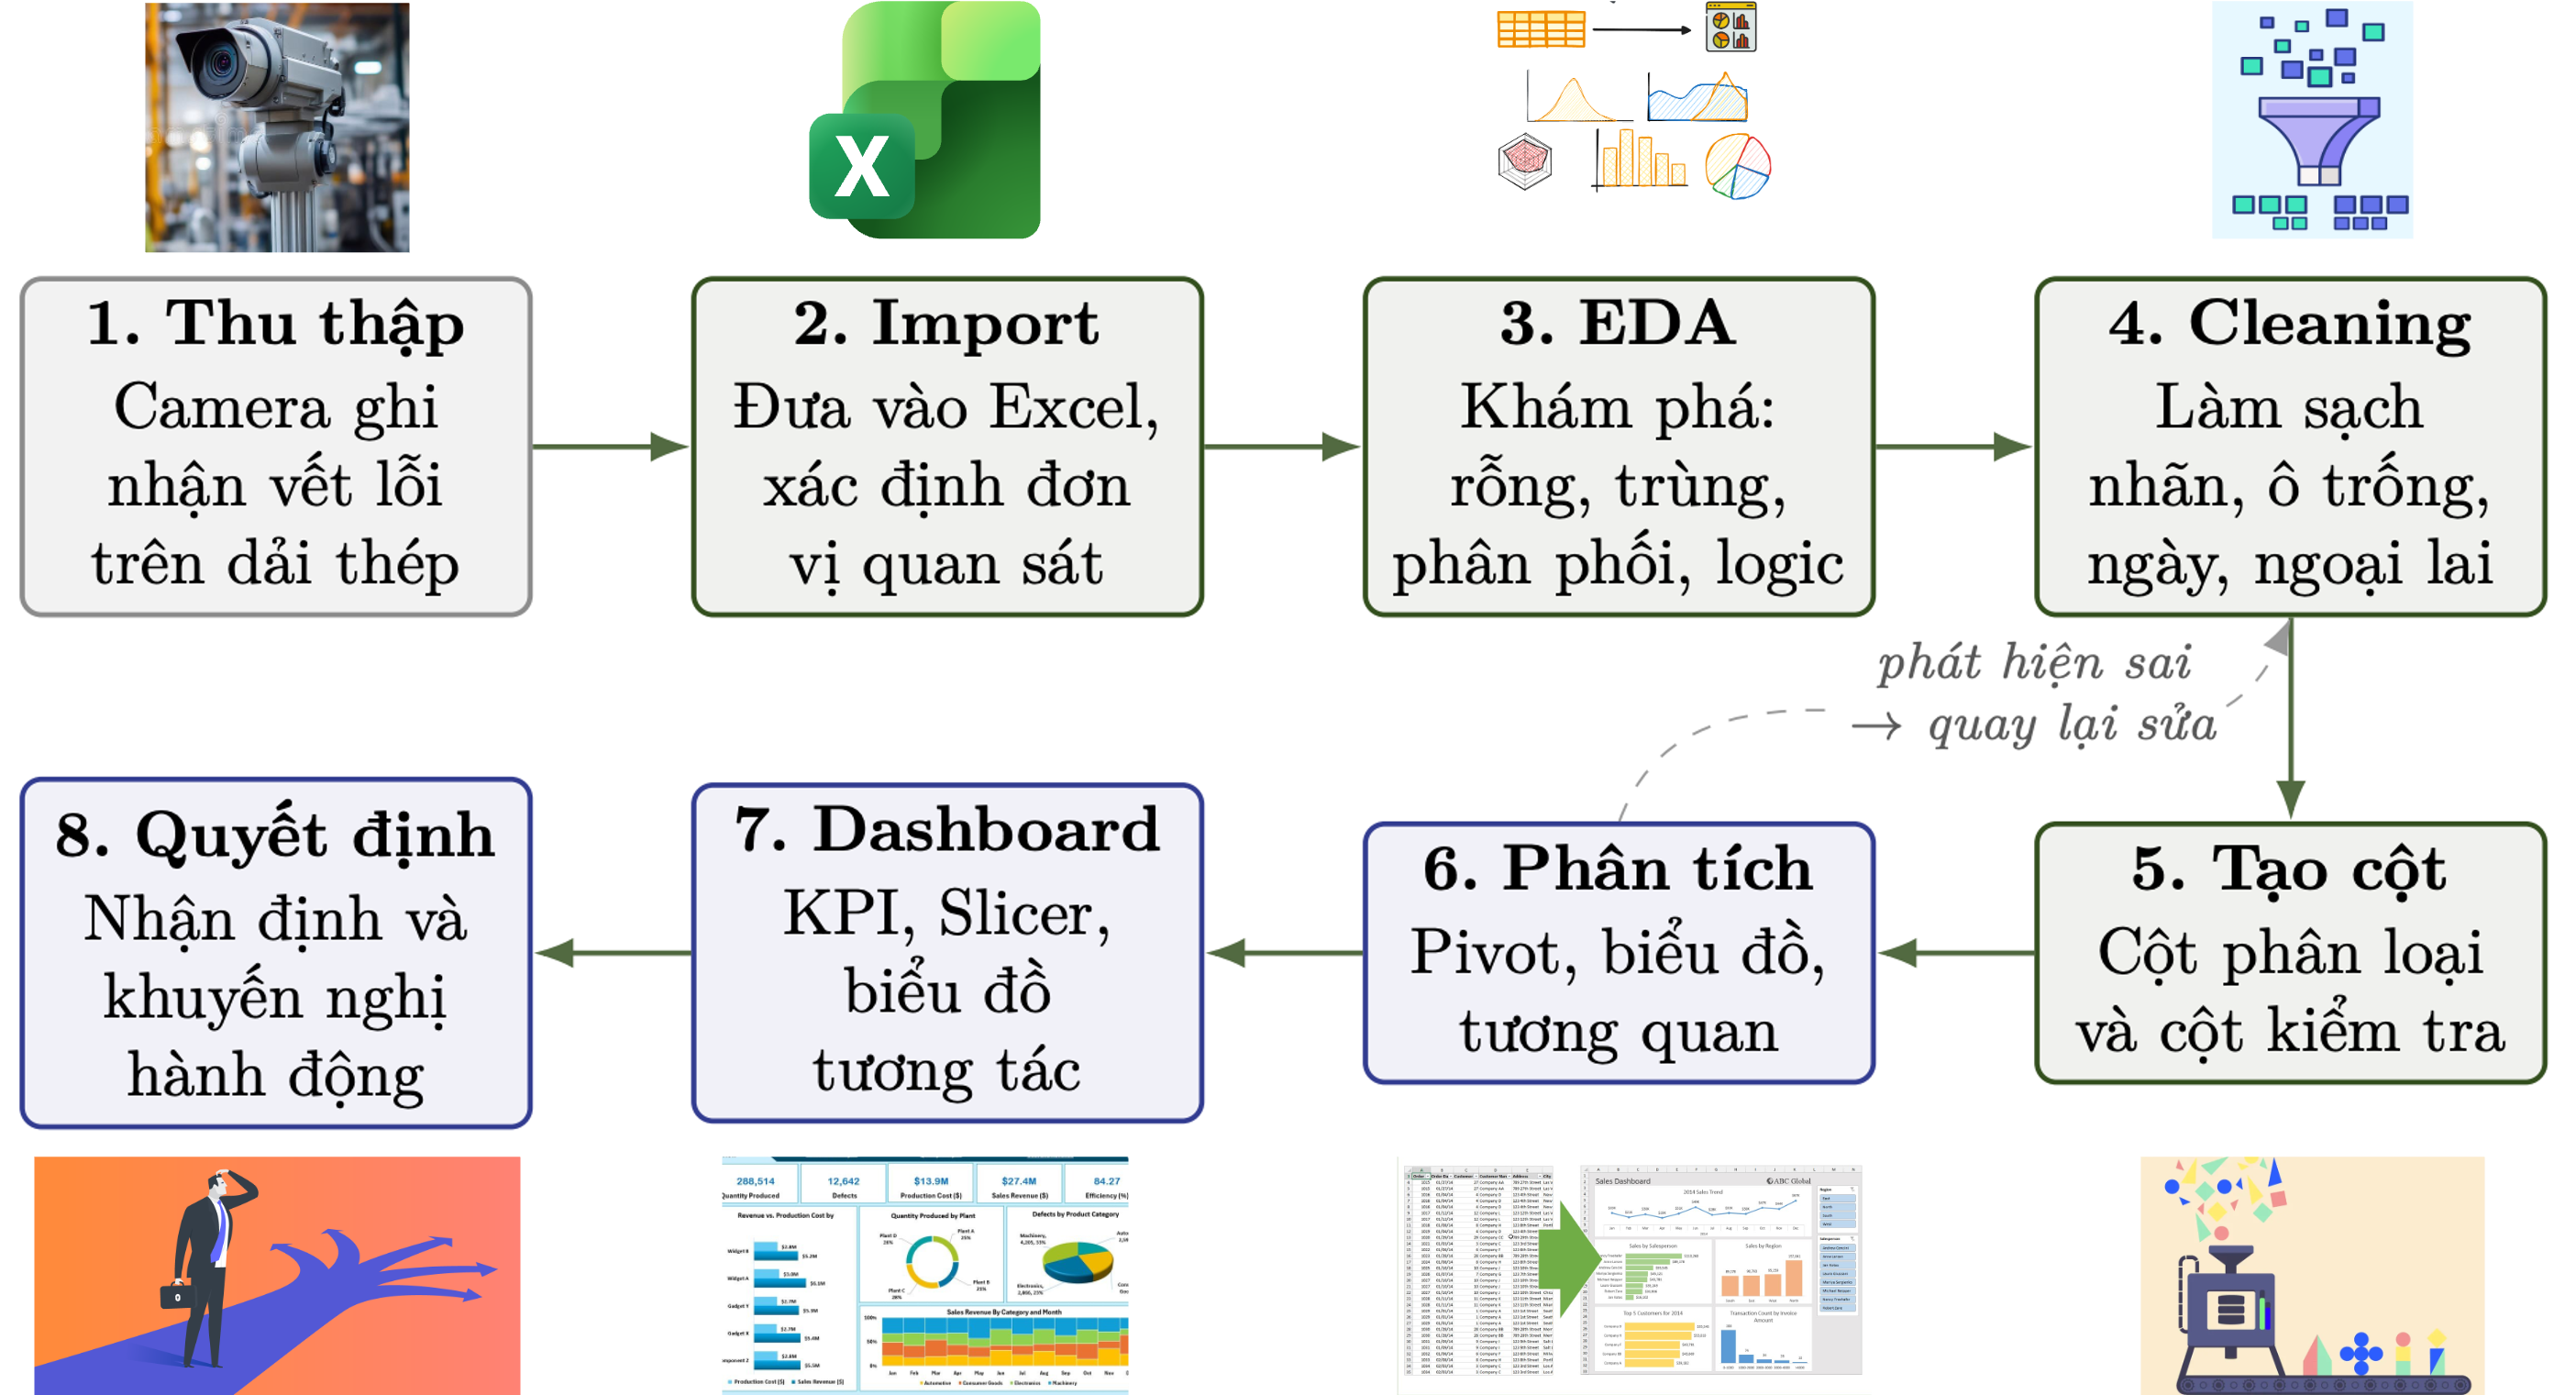
\includegraphics[width=0.94\linewidth]{Figures/overview.png}
\end{figure}


\clearpage
\tableofcontents
\clearpage


\part{Nền tảng lý thuyết}

\section{Giới thiệu}

\subsection{Vấn đề đặt ra}

Có một bảng ghi nhận lỗi không đồng nghĩa với việc hiểu được lỗi. Bảng trả lời câu hỏi \emph{có bao nhiêu vết lỗi và chúng trông như thế nào}, nhưng không tự trả lời được ba câu hỏi mà người quản lý sản xuất thực sự cần.

\begin{itemize}
  \item Trong bảy loại lỗi đang được ghi nhận, loại nào chiếm phần lớn và đáng xem xét trước?
  \item Lỗi có trải đều trên mọi sản phẩm, hoặc tập trung vào một dòng thép, một khoảng độ dày cụ thể? Nếu có tập trung, đó là một mối liên hệ đáng mang ra hiện trường kiểm chứng, chưa phải bằng chứng về nguyên nhân.
  \item Các đặc trưng đang được ghi nhận (kích thước, hình dạng, độ sáng) có tách được các loại lỗi đủ rõ để thử một quy tắc nhận diện hay không?
\end{itemize}

\noindent Một bảng dữ liệu nằm im trong file Excel không tự trả lời được những câu hỏi đó. Khoảng cách giữa \emph{dữ liệu đã có} và \emph{câu hỏi cần trả lời} chính là phần việc của bài phân tích này.

\subsection{Mục tiêu và sản phẩm bàn giao}

Báo cáo đặt ra ba mục tiêu, mỗi mục tiêu gắn với một sản phẩm cụ thể có thể kiểm chứng được.

\begin{center}
\begin{tabular}{@{}p{0.5cm} p{6.6cm} p{8.6cm}@{}}
\toprule
 & \textbf{Mục tiêu} & \textbf{Sản phẩm bàn giao} \\
\midrule
1 & Đưa bảng dữ liệu thô về trạng thái đủ tin cậy để mọi con số tính ra đều có nghĩa & Bảng dữ liệu đã làm sạch, kèm các cột kiểm tra cho phép chạy lại và xác minh từng bước can thiệp (Mục VI) \\
\addlinespace[4pt]
2 & Mô tả phân bố lỗi theo cơ cấu loại lỗi, dòng thép, độ dày và đặc trưng độ sáng, và đo các mối liên hệ giữa chúng trong mẫu & Ba phân tích có bằng chứng bằng bảng Pivot và biểu đồ (Mục VII) \\
\addlinespace[4pt]
3 & Chuyển kết quả phân tích thành danh sách việc cần kiểm chứng tiếp, xếp theo mức độ chắc chắn của bằng chứng & Dashboard theo dõi, danh sách phát hiện phân theo ba mức tin cậy và kế hoạch kiểm chứng ba giai đoạn (Mục VIII đến X) \\
\bottomrule
\end{tabular}
\end{center}

\noindent Toàn bộ báo cáo được thực hiện trên Microsoft Excel, sử dụng công thức, Pivot Table, Data Analysis ToolPak và Slicer. Việc giới hạn công cụ ở Excel là chủ ý, vì nó buộc mọi bước xử lý phải hiện ra thành một công thức nhìn thấy được trong ô, thay vì ẩn trong một dòng lệnh.

\subsection{Phạm vi và giới hạn}

Năm giới hạn dưới đây quyết định cách đọc mọi con số ở các phần sau, nên được nêu ngay từ đầu thay vì đặt ở phần kết luận.

\begin{enumerate}
  \item \textbf{Đơn vị quan sát là vết lỗi, không phải tấm thép.} Mỗi dòng dữ liệu mô tả một vết lỗi. Bảng không cho biết một tấm thép có bao nhiêu vết lỗi, cũng không cho biết có bao nhiêu tấm thép hoàn toàn không lỗi.
  \item \textbf{Không có mẫu số.} Vì không biết tổng sản lượng đã sản xuất, báo cáo không thể tính \emph{tỷ lệ lỗi} theo nghĩa thông thường (số tấm lỗi trên tổng số tấm). Mọi phát biểu dạng \emph{lỗi X chiếm 34,67\%} đều là tỷ trọng \emph{trong nội bộ tập vết lỗi}, không phải xác suất một tấm thép bị lỗi X.
  \item \textbf{Dữ liệu quan sát, không phải thí nghiệm.} Nhóm không can thiệp vào dây chuyền để tạo dữ liệu. Do đó mọi liên hệ tìm được là tương quan, không phải quan hệ nhân quả. Khi báo cáo viết \emph{K\_Scatch gắn với thép A400 ở độ dày 40}, đó là một mô tả cần được kiểm chứng lại tại hiện trường, chưa phải một kết luận về nguyên nhân.
  \item \textbf{Không có tài liệu về cách đo và cách gán nhãn.} Nguồn công bố dữ liệu không kèm định nghĩa của bảy nhãn lỗi, không nêu đơn vị đo của bất kỳ biến nào, và không mô tả thiết bị đã sinh ra các con số. Vì vậy báo cáo không phát biểu về cơ chế vật lý của từng loại lỗi, và không gắn đơn vị cho các biến số.
  \item \textbf{Cột ngày là biến mô phỏng.} \texttt{Production\_Date} không thuộc bộ dữ liệu gốc mà được bổ sung để thực hành thao tác lọc theo thời gian. Cột này chỉ nhận 5 giá trị ngày, và không được dùng để nói về xu hướng theo thời gian hoặc tính mùa vụ.
\end{enumerate}

\begin{guidelinebox}{Vì sao phải nêu giới hạn trước khi phân tích}
Nêu giới hạn ở đầu báo cáo giúp xác định trước phạm vi những phát biểu được phép đưa ra, và việc đó không làm giảm giá trị của kết quả. Một bài phân tích sai không phải vì tính toán sai, mà thường vì kết luận vượt quá điều dữ liệu có thể chứng minh. Danh sách trên chính là hàng rào cho phần Nhận định và Khuyến nghị ở cuối báo cáo.
\end{guidelinebox}

\subsection{Cấu trúc báo cáo}

\begin{center}
\begin{tabular}{@{}p{1.1cm} p{5.2cm} p{9.4cm}@{}}
\toprule
\textbf{Mục} & \textbf{Tên} & \textbf{Trả lời câu hỏi} \\
\midrule
\multicolumn{3}{@{}l}{\textbf{Mục A. Nền tảng lý thuyết}} \\
\addlinespace[2pt]
I    & Giới thiệu & Vì sao cần bài phân tích này, và nó cam kết làm gì \\
II   & Hành trình của dữ liệu & Dữ liệu đi qua những bước nào để trở thành quyết định \\
III  & Hiểu về bối cảnh sản xuất thép & Cần biết gì về sản xuất thép để đọc đúng các con số \\
IV   & Hiểu về bộ dữ liệu & 29 cột là gì, đo cái gì, tin được đến đâu \\
V    & Các câu hỏi trung tâm & Báo cáo sẽ trả lời chính xác những câu hỏi nào \\
\addlinespace[5pt]
\multicolumn{3}{@{}l}{\textbf{Mục B. Thực hành trên Excel}} \\
\addlinespace[2pt]
VI   & Chuẩn bị dữ liệu & Bảng dữ liệu được làm sạch và chuẩn hóa như thế nào \\
VII  & Phân tích & Ba trục phân tích gồm cơ cấu lỗi, độ sáng và độ dày \\
VIII & Dashboard & Kết quả được trực quan hóa để theo dõi thường xuyên ra sao \\
IX   & Nhận định & Những phát hiện nào chắc, những phát hiện nào còn phải kiểm \\
X    & Khuyến nghị & Cần kiểm chứng những gì tiếp theo, theo thứ tự nào \\
\addlinespace[5pt]
\multicolumn{3}{@{}l}{\textbf{Cuối bài}} \\
\addlinespace[2pt]
 & Tài liệu tham khảo & Tải dữ liệu và file Excel lời giải ở đâu, và bài dựa trên nguồn nào \\
\bottomrule
\end{tabular}
\end{center}

\noindent Báo cáo chia thành hai phần lớn. Mục A (mục I đến V) đặt nền về bối cảnh, quy trình, kiến thức ngành, hiểu biết về dữ liệu và bộ câu hỏi. Mục B (mục VI đến X) là phần thực thi trên dữ liệu thật. Phần phụ lục cung cấp link tải dữ liệu và file lời giải để tái lập toàn bộ kết quả, cùng chỗ dự phòng cho các phụ lục khác (ví dụ bộ prompt) khi cần bổ sung. Người đọc cần kết quả nhanh có thể đọc thẳng Mục IX và X; người đọc muốn kiểm chứng cách làm nên đọc tuần tự.

% =====================================================================
\clearpage
\section{Hành trình của dữ liệu}

Một bài phân tích là một hành trình có hướng, bắt đầu từ một hiện tượng vật lý trên bề mặt thép và kết thúc ở một quyết định của người quản lý sản xuất. Các thao tác Excel trong báo cáo nối tiếp nhau theo đúng hành trình đó. Mục này mô tả toàn bộ hành trình trước, để khi đọc các phần chi tiết phía sau, mỗi thao tác đều có chỗ đứng rõ ràng trong bức tranh chung.

\subsection{Sơ đồ tổng thể}

\begin{figure}[H]
\centering
\begin{tikzpicture}[
  font=\footnotesize,
  bx/.style={rectangle, rounded corners=3pt, draw=aivnGreen, thick,
             fill=aivnGreen!8, text width=2.55cm, minimum height=1.25cm,
             align=center, inner sep=3pt},
  arr/.style={-{Latex[length=2.2mm]}, draw=aivnGreen!85, thick}
]
% ---- Hàng 1 ----
\node[bx, fill=black!5, draw=black!45] (b1) at (0,0)
      {\textbf{1. Thu thập}\\[1pt] Camera ghi nhận vết lỗi trên dải thép};
\node[bx] (b2) at (3.65,0)  {\textbf{2. Import}\\[1pt] Đưa vào Excel, xác định đơn vị quan sát};
\node[bx] (b3) at (7.30,0)  {\textbf{3. EDA}\\[1pt] Khám phá: rỗng, trùng, phân phối, logic};
\node[bx] (b4) at (10.95,0) {\textbf{4. Cleaning}\\[1pt] Làm sạch nhãn, ô trống, ngày, ngoại lai};
% ---- Hàng 2 ----
\node[bx] (b5) at (10.95,-2.75) {\textbf{5. Tạo cột}\\[1pt] Cột phân loại và cột kiểm tra};
\node[bx, fill=brandIndigo!7, draw=brandIndigo] (b6) at (7.30,-2.75)
      {\textbf{6. Phân tích}\\[1pt] Pivot, biểu đồ, tương quan};
\node[bx, fill=brandIndigo!7, draw=brandIndigo] (b7) at (3.65,-2.75)
      {\textbf{7. Dashboard}\\[1pt] KPI, Slicer, biểu đồ tương tác};
\node[bx, fill=brandIndigo!7, draw=brandIndigo] (b8) at (0,-2.75)
      {\textbf{8. Quyết định}\\[1pt] Nhận định và khuyến nghị hành động};
% ---- Mũi tên ----
\draw[arr] (b1) -- (b2);
\draw[arr] (b2) -- (b3);
\draw[arr] (b3) -- (b4);
\draw[arr] (b4) -- (b5);
\draw[arr] (b5) -- (b6);
\draw[arr] (b6) -- (b7);
\draw[arr] (b7) -- (b8);
% ---- Vòng lặp kiểm chứng ngược ----
\draw[dashed, -{Latex[length=2mm]}, gray!80] (b6.north) to[out=70,in=-115] (b4.south);
\node[font=\scriptsize\itshape, text=black!65, align=center, fill=white, inner sep=1pt]
      at (9.55,-1.35) {phát hiện sai\\ $\rightarrow$ quay lại sửa};
% ---- Chú giải ----
\fill[black!5, draw=black!45]            (0.15,-4.12) rectangle ++(0.26,0.26);
\node[anchor=west, font=\scriptsize] at  (0.50,-3.99) {Nguồn dữ liệu};
\fill[aivnGreen!8, draw=aivnGreen]       (3.30,-4.12) rectangle ++(0.26,0.26);
\node[anchor=west, font=\scriptsize] at  (3.65,-3.99) {Chuẩn bị dữ liệu (Mục VI)};
\fill[brandIndigo!7, draw=brandIndigo]   (7.60,-4.12) rectangle ++(0.26,0.26);
\node[anchor=west, font=\scriptsize] at  (7.95,-3.99) {Khai thác dữ liệu (Mục VII--X)};
\end{tikzpicture}
\begin{figurecaptionmodern1}
\capfig{Hành trình của dữ liệu, từ vết lỗi trên tấm thép đến quyết định sản xuất.}
\end{figurecaptionmodern1}
\end{figure}

\subsection{Nội dung từng bước}

\begin{center}
\small
\begin{tabular}{@{}p{0.45cm} p{2.6cm} p{5.9cm} p{6.5cm}@{}}
\toprule
 & \textbf{Bước} & \textbf{Câu hỏi cần trả lời} & \textbf{Kết quả bàn giao} \\
\midrule
1 & Thu thập & Dữ liệu sinh ra từ đâu, và nguồn cho biết những gì? & Cách hiểu làm việc cho từng nhóm biến (Mục III) \\
\addlinespace[3pt]
2 & Import và khảo sát & Bảng có bao nhiêu dòng, bao nhiêu cột, mỗi dòng đại diện cho cái gì? & Từ điển dữ liệu 29 cột (Mục IV) \\
\addlinespace[3pt]
3 & EDA & Dữ liệu có vấn đề gì trong số thiếu, trùng, sai định dạng và giá trị vô lý? & Danh sách vấn đề kèm số lượng cụ thể (Mục VI) \\
\addlinespace[3pt]
4 & Cleaning & Sửa như thế nào để không làm mất thông tin thật? & Bảng đã sạch, có dấu vết can thiệp (Mục VI) \\
\addlinespace[3pt]
5 & Tạo cột bổ sung & Cần biến nào mà bảng gốc chưa có sẵn? & Cột \texttt{SteelType} và các cột kiểm tra (Mục VI) \\
\addlinespace[3pt]
6 & Phân tích & Các câu hỏi ở Mục V được trả lời bằng bằng chứng nào? & Bảng Pivot và biểu đồ (Mục VII) \\
\addlinespace[3pt]
7 & Dashboard & Làm sao để người không phân tích vẫn theo dõi được? & Một màn hình có KPI và bộ lọc (Mục VIII) \\
\addlinespace[3pt]
8 & Quyết định & Phát hiện nào đủ chắc, và cần kiểm chứng gì tiếp? & Nhận định phân ba mức tin cậy và kế hoạch kiểm chứng (Mục IX đến X) \\
\bottomrule
\end{tabular}
\end{center}

\subsection{Hai nguyên tắc xuyên suốt}

Hành trình trên có thể trình bày như một đường thẳng, nhưng thực tế nó vận hành theo hai nguyên tắc mà nếu bỏ qua, kết quả cuối sẽ sai mà không ai biết.\medskip

\noindent \textbf{Nguyên tắc 1. Thứ tự các bước làm sạch không tùy tiện}

\noindent Bốn nhóm vấn đề của bảng dữ liệu này phải được xử lý theo đúng một thứ tự cố định, gồm chuẩn hóa nhãn, loại dòng trùng, điền ô trống, rồi mới rà giá trị ngoại lai. Đảo thứ tự sẽ sinh ra sai lệch dây chuyền.

\begin{itemize}
  \item Nếu \emph{điền ô trống trước khi gom nhãn}, thì khi điền theo đặc trưng của nhóm lỗi, một loại lỗi đang bị tách thành nhiều biến thể sẽ cho ra giá trị điền sai.
  \item Nếu \emph{tính ngoại lai trước khi loại dòng trùng}, thì các dòng bị nhân đôi làm lệch tứ phân vị, kéo theo ngưỡng IQR sai, dẫn tới gắn cờ nhầm.
  \item Nếu \emph{tính chỉ số phái sinh trước khi sửa tọa độ gốc}, thì sai số được nhân bản sang các cột mới và trở nên khó truy vết hơn.
\end{itemize}

\noindent \textbf{Nguyên tắc 2. Mỗi bước phải để lại một chốt kiểm tra chạy lại được}

\noindent Không bước nào được phép tin vào kết quả của bước trước chỉ vì bước đó đã được thực hiện. Cách làm xuyên suốt báo cáo là sau mỗi can thiệp phải dựng một công thức đếm hoặc một khoảng giá trị kỳ vọng, sao cho nếu dữ liệu bị sửa nhầm về sau, con số kiểm tra sẽ lệch khỏi giá trị kỳ vọng ngay lập tức. Mục VI dùng ba cột \texttt{Log\_Y\_Check}, \texttt{Empty\_Check} và \texttt{Orientation\_Check}, cả ba đều phải luôn trả về 0 ô lệch, cùng với hai phép \texttt{SUMPRODUCT} kiểm tra vị trí trục X cũng phải luôn trả về 0.

\subsection{Một sự cố thực tế trong quá trình thực hiện báo cáo}

Sơ đồ ở trên có một mũi tên nét đứt đi ngược từ bước Phân tích về bước Cleaning. Mũi tên đó không phải để trang trí. Trong quá trình làm bài, khi rà soát giá trị ngoại lai của ba cột chỉ số phái sinh, nhóm phát hiện bốn ô trống của cột \texttt{Orientation\_Index} ở bước xử lý dữ liệu trống trước đó đã được điền bằng một công thức trông hợp lý nhưng sai so với định nghĩa của cột. Bốn giá trị sai này nằm gọn trong miền hợp lệ nên không một phép thống kê nào phát hiện được; chỉ có phép tính lại từ tọa độ gốc mới chỉ ra. Toàn bộ diễn biến được ghi lại ở Mục VI.

\noindent Đây là lý do báo cáo trình bày quy trình như một vòng lặp có kiểm chứng, chứ không như một danh sách công việc đã hoàn tất và không cần xem lại.

% =====================================================================
\clearpage
\section{Hiểu về bối cảnh sản xuất thép}

Cùng một con số có thể mang hai ý nghĩa hoàn toàn khác nhau tùy vào việc người đọc có biết nó sinh ra từ đâu hay không. Với bộ dữ liệu này, câu trả lời chỉ đến được một nửa. Tên các cột cho thấy đây là kết quả của một hệ thống đo ảnh, vì các cột tọa độ mô tả một khung chữ nhật, \texttt{Pixels\_Areas} đếm theo điểm ảnh, ba cột \texttt{Luminosity} đo độ sáng. Nhưng nguồn công bố \textbf{không kèm tài liệu mô tả thiết bị, quy trình đo hoặc định nghĩa của bảy nhãn lỗi}.

\noindent Mục này vì vậy làm hai việc tách bạch. Nó nêu cách hiểu làm việc cho từng nhóm biến, đủ để người đọc biết mỗi cột đang nói về cái gì và đọc đúng các con số ở phần sau. Đồng thời nó ghi rõ chỗ nào là suy ra từ tên biến và từ chính dữ liệu, chỗ nào là kiến thức ngành đưa vào từ bên ngoài. Năm khái niệm được trình bày theo đúng thứ tự một bản ghi được tạo ra, gồm loại lỗi và loại thép mà bản ghi đó thuộc về, nhóm chỉ số hình học, độ sáng, và cuối cùng là độ dày tấm thép.

\begin{guidelinebox}{Cách đọc mục này}
Không một phát biểu nào trong Mục III được dùng làm bằng chứng ở Mục IX. Các phát biểu về cơ chế vật lý ở đây chỉ có một vai trò, là gợi ra giả thuyết để đi kiểm chứng tại hiện trường. Bằng chứng của báo cáo nằm ở Mục VII, và toàn bộ là bằng chứng mô tả về phân bố và về liên hệ trong mẫu.
\end{guidelinebox}

\subsection{Loại lỗi \textit{Faults} (Lỗi trên tấm thép được ghi nhận như thế nào?)}

\texttt{Faults} là biến mục tiêu của bộ dữ liệu, nhận đúng một trong bảy giá trị. Bảng dưới đây liệt kê bảy nhãn kèm cách hiểu suy ra từ chính tên nhãn, và kèm số bản ghi đo được trong dữ liệu đã làm sạch. Cột cuối là thứ duy nhất trong bảng không phải suy đoán.

\begin{center}
\small
\begin{tabular}{@{}p{2.8cm} p{9.4cm} r@{}}
\toprule
\textbf{Nhãn} & \textbf{Cách hiểu suy ra từ tên nhãn} & \textbf{Số bản ghi} \\
\midrule
\texttt{Other\_Faults} & Nhóm gộp các trường hợp còn lại. Không phải một loại lỗi, mà là tập hợp mọi bản ghi không rơi vào sáu nhãn kia & 673 \\
\addlinespace[3pt]
\texttt{Bumps}        & Chỗ lồi hoặc gồ trên bề mặt & 402 \\
\addlinespace[3pt]
\texttt{K\_Scatch}    & Vết xước, phân biệt với \texttt{Z\_Scratch} bằng chữ cái đầu trong tên nhãn & 391 \\
\addlinespace[3pt]
\texttt{Z\_Scratch}   & Vết xước dạng vạch & 190 \\
\addlinespace[3pt]
\texttt{Pastry}       & Mảng bề mặt không đồng nhất, kết cấu khác vùng xung quanh & 158 \\
\addlinespace[3pt]
\texttt{Stains}       & Vết ố, vùng đổi màu & 72 \\
\addlinespace[3pt]
\texttt{Dirtiness}    & Bẩn bám trên bề mặt & 55 \\
\midrule
\textbf{Tổng} & & \textbf{1.941} \\
\bottomrule
\end{tabular}
\end{center}

\begin{notebox}
Nguồn công bố \textbf{không kèm định nghĩa chính thức} của bảy nhãn này, cũng không kèm định nghĩa của các chỉ số đặc trưng. Cột giữa của bảng trên vì vậy là \textbf{cách hiểu làm việc} suy ra từ tên nhãn, không phải trích dẫn từ tài liệu kỹ thuật. Báo cáo không phát biểu về cơ chế vật lý sinh ra từng loại lỗi, vì không có nguồn nào cho phép làm điều đó. Khi triển khai thực tế, bước đầu tiên phải là ngồi lại với bộ phận QC để chốt định nghĩa từng nhãn.

\noindent Nhãn \texttt{K\_Scatch} là cách viết có sẵn trong bộ dữ liệu gốc (thiếu chữ \emph{r} so với \emph{scratch}). Báo cáo giữ nguyên cách viết này để đối chiếu được với nguồn, và không xem đây là một biến thể cần gom nhãn.
\end{notebox}

\noindent Điều dữ liệu \emph{có thể} nói, và Mục VII sẽ đo cụ thể, là mức độ \textbf{tập trung} của từng nhãn. Một nhãn trải đều trên mọi dòng thép và mọi khoảng độ dày cho thấy một hiện tượng phân tán. Ngược lại, một nhãn dồn gần như toàn bộ vào một dòng thép, ở một mức độ dày, với độ biến thiên rất nhỏ, là một khuôn có hệ thống trong dữ liệu. Khuôn đó chưa nói được nguyên nhân, nhưng nó chỉ đúng chỗ cần mang ra hiện trường kiểm chứng, và đó là logic dẫn tới phát hiện về \texttt{K\_Scatch} ở Mục IX.

\begin{misconceptionbox}{Loại lỗi $\neq$ mức độ nghiêm trọng}
Người mới thường mặc định \texttt{Other\_Faults} là loại lỗi nhẹ nhất vì nó đứng cuối trong tên gọi (\textit{other}, nghĩa là \emph{khác}). Thực tế ngược lại. Đây là nhãn chiếm số lượng \textbf{nhiều nhất} trong toàn bộ dữ liệu (673 trên 1.941 vết, 34,67\%), vì nó gộp mọi vết lỗi \textbf{không khớp} với sáu khuôn hình dạng chuẩn còn lại. Nhãn này mô tả phần dư của hệ thống phân loại, không mô tả một loại khuyết tật vật lý cụ thể.
\end{misconceptionbox}

\noindent \colorbox{LimeGreen}{\textbf{Insight}} Vì \texttt{Faults} là một nhãn phân loại (biến mục tiêu) chứ không phải một thang đo liên tục, số lượng lớn của một nhãn chỉ nói lên rằng nhãn đó được gán nhiều hơn trong dữ liệu đã thu thập, không nói lên nó nguy hiểm hơn. Mọi thống kê tính trên \texttt{Other\_Faults} (trung bình độ dày, trung bình độ sáng) đều là trung bình của nhiều hiện tượng khác nhau cộng lại, nên không diễn giải được như một đặc trưng riêng biệt; đây là nền tảng cho khuyến nghị tách nhỏ nhóm này ở Mục X.

\subsection{Loại thép \textit{TypeOfSteel\_A300} và \textit{TypeOfSteel\_A400} (Vì sao mỗi vết lỗi lại gắn với một loại thép cụ thể?)}

Bộ dữ liệu ghi nhận hai dòng thép, lưu dưới dạng hai cột nhị phân \texttt{TypeOfSteel\_A300} và \texttt{TypeOfSteel\_A400} (giá trị 0 hoặc 1). Tài liệu gốc không nêu rõ hai mã này tương ứng với mác thép hoặc tiêu chuẩn nào. Những gì có thể khẳng định là đây chỉ là hai họ sản phẩm được sản xuất trên cùng hệ thống nhưng có đặc điểm khác nhau, và mỗi vết lỗi thuộc về đúng một trong hai dòng.

\begin{misconceptionbox}{TypeOfSteel\_A300 và TypeOfSteel\_A400 $\neq$ hai biến độc lập}
Vì mỗi cột chỉ nhận giá trị 0 hoặc 1, người mới dễ đưa cả hai cột cùng lúc vào một mô hình hồi quy như hai đặc trưng riêng biệt. Thực chất đây là một phép mã hoá one-hot của \textbf{cùng một biến duy nhất} (\emph{loại thép}). Một tấm thép luôn là A300 hoặc A400, không thể là cả hai hoặc không là gì cả. Đưa cả hai cột vào cùng một mô hình tuyến tính sẽ gây đa cộng tuyến hoàn hảo (perfect collinearity).
\end{misconceptionbox}

\noindent \colorbox{LimeGreen}{\textbf{Insight}} Điều đáng chú ý về mặt phương pháp là chính \emph{dữ liệu} sẽ cho biết hai dòng này khác nhau ra sao. Nếu một loại lỗi xuất hiện gần như tuyệt đối trên một dòng thép, sự phân tách đó là một khuôn có hệ thống, đáng để đi tìm xem hai dòng khác nhau ở điều kiện sản xuất nào. Bản thân nó chưa cho biết điều kiện đó là gì, vì không có tài liệu mô tả và cũng không có biến vận hành nào trong bảng. Một biến chỉ nhận hai giá trị 0 và 1 vẫn có thể là tín hiệu dự đoán rất mạnh. Kết quả cụ thể của bộ dữ liệu này, với K\_Scatch gần như chỉ nằm trên A400 và Z\_Scratch chủ yếu trên A300, được trình bày ở Mục VII.1.

\subsection{Nhóm chỉ số hình học về toạ độ, diện tích và chu vi (Camera đo một vết lỗi bằng cách nào?)}

Tên và miền giá trị của nhóm cột này khớp với đầu ra của một quy trình thị giác máy tính gồm bốn bước. Đây là cách hiểu làm việc suy ra từ chính tên biến, không phải mô tả lấy từ tài liệu của nguồn.

\begin{enumerate}
  \item Camera quét liên tục bề mặt dải thép dưới một nguồn sáng có cường độ ổn định.
  \item Phần mềm so sánh độ sáng từng điểm ảnh với nền thép lành; vùng nào lệch khỏi nền quá ngưỡng thì được đánh dấu là một vết lỗi.
  \item Với mỗi vùng đã khoanh, hệ thống dựng một khung chữ nhật nhỏ nhất bao trọn vết lỗi (bounding box) rồi đo tọa độ khung bao, số điểm ảnh, chu vi và các thống kê độ sáng.
  \item Bộ phân loại gán vùng đó vào một trong bảy nhãn lỗi.
\end{enumerate}

\noindent Toàn bộ nhóm cột hình học trong bảng dữ liệu sinh ra từ đúng thao tác đo ở Bước 3 trên. Hai cột \texttt{X\_Minimum}/\texttt{X\_Maximum} là hai cạnh khung theo chiều ngang khung ảnh, \texttt{Y\_Minimum}/\texttt{Y\_Maximum} là hai cạnh theo chiều dọc băng chuyền, \texttt{Pixels\_Areas} đếm số điểm ảnh thuộc vết lỗi, còn \texttt{X\_Perimeter}/\texttt{Y\_Perimeter} đo chu vi chiếu theo từng trục.

\noindent Hình dưới đây trình bày quan hệ giữa hiện tượng vật lý và các con số trong bảng dữ liệu.

\begin{figure}[H]
\centering
\begin{tikzpicture}[font=\footnotesize]
% Dải thép
\fill[black!7] (0,0) rectangle (10.5,4.4);
\draw[black!30] (0,0) rectangle (10.5,4.4);
\node[anchor=north west, text=black!55, font=\scriptsize] at (0.15,4.28)
      {Ảnh bề mặt dải thép do camera ghi nhận};
% Vết lỗi
\begin{scope}
  \clip (0,0) rectangle (10.5,4.4);
  \fill[aivnGreen!65, rotate around={22:(4.2,2.3)}] (4.2,2.3) ellipse (1.3 and 0.48);
\end{scope}
% Khung bao
\draw[dashed, red!70!black, thick] (2.80,1.55) rectangle (5.60,3.05);
% Guides trục X
\draw[black!45, dotted] (2.80,1.55) -- (2.80,0.55);
\draw[black!45, dotted] (5.60,1.55) -- (5.60,0.55);
\draw[{Latex[length=1.6mm]}-{Latex[length=1.6mm]}, black!70] (2.80,0.78) -- (5.60,0.78);
\node[below, font=\scriptsize] at (4.20,0.75) {$dX$};
\node[below left, font=\scriptsize, text=black!75] at (2.88,0.55) {\texttt{X\_Minimum}};
\node[below right, font=\scriptsize, text=black!75] at (5.52,0.55) {\texttt{X\_Maximum}};
% Guides trục Y
\draw[black!45, dotted] (2.80,1.55) -- (-0.2,1.55);
\draw[black!45, dotted] (2.80,3.05) -- (-0.2,3.05);
\draw[{Latex[length=1.6mm]}-{Latex[length=1.6mm]}, black!70] (-0.05,1.55) -- (-0.05,3.05);
\node[left, font=\scriptsize] at (-0.1,2.3) {$dY$};
\node[left, font=\scriptsize, text=black!75] at (-0.25,1.55) {\texttt{Y\_Minimum}};
\node[left, font=\scriptsize, text=black!75] at (-0.25,3.05) {\texttt{Y\_Maximum}};
% Chú thích các đại lượng đo được
\node[anchor=west, font=\scriptsize, text=black!80, fill=white, rounded corners=2pt,
      inner sep=3pt, text width=3.95cm, align=left] (a1) at (6.10,3.45)
      {\texttt{Pixels\_Areas} là số điểm ảnh thuộc vết lỗi};
\node[anchor=west, font=\scriptsize, text=black!80, fill=white, rounded corners=2pt,
      inner sep=3pt, text width=3.95cm, align=left] (a2) at (6.10,2.30)
      {\texttt{X\_Perimeter} và \texttt{Y\_Perimeter} là chu vi chiếu theo hai trục};
\node[anchor=west, font=\scriptsize, text=black!80, fill=white, rounded corners=2pt,
      inner sep=3pt, text width=3.95cm, align=left] (a3) at (6.10,1.05)
      {\texttt{Sum/Min/Max\_of\_Luminosity} là thống kê độ sáng của chính các điểm ảnh đó};
\draw[black!50, -{Latex[length=1.6mm]}] (a2.west) -- (5.72,2.30);
% Chiều rộng băng tải
\draw[{Latex[length=1.6mm]}-{Latex[length=1.6mm]}, black!60] (0,-0.38) -- (10.5,-0.38);
\node[below, font=\scriptsize, text=black!75] at (5.25,-0.38) {\texttt{Length\_of\_Conveyer} (chiều rộng vùng quét)};
\end{tikzpicture}
\begin{figurecaptionmodern}
\capfig{Cách một vết lỗi trên bề mặt thép được chuyển thành các con số trong bảng dữ liệu. Mọi cột hình học đều được đo trên khung bao chữ nhật nhỏ nhất chứa vết lỗi, không đo trực tiếp trên hình dạng thật của vết lỗi.}
\end{figurecaptionmodern}
\end{figure}

\noindent Ba nhận xét rút ra từ hình này, cả ba đều được dùng lại ở các mục sau.

\begin{itemize}
  \item \textbf{Khung bao luôn lớn hơn hoặc bằng vết lỗi.} Tỷ lệ phần diện tích khung \emph{không} thuộc vết lỗi chính là ý nghĩa của cột \texttt{Empty\_Index}, và vì là một tỷ lệ nên nó bắt buộc nằm trong đoạn $[0;1]$; đây chính là cơ sở để phát hiện giá trị sai ở Mục VI.
  \item \textbf{Toạ độ X bị chặn bởi chiều rộng vùng quét.} Không vết lỗi nào có thể có tọa độ X vượt quá \texttt{Length\_of\_Conveyer}. Đây là một ràng buộc logic kiểm tra được bằng một công thức duy nhất.
  \item \textbf{Độ sáng được đo trên đúng tập điểm ảnh của vết lỗi.} Vì vậy \texttt{Maximum\_of\_Luminosity} không bao giờ nhỏ hơn \texttt{Minimum\_of\_Luminosity}; đây là một ràng buộc nữa để kiểm tra tính toàn vẹn.
\end{itemize}

\begin{misconceptionbox}{\texttt{Y\_Maximum} lớn $\neq$ tấm thép dài}
Vì \texttt{Y\_Minimum}/\texttt{Y\_Maximum} có thể lên tới hàng trăm nghìn, người mới dễ hiểu nhầm đây là chiều dài vật lý của tấm thép. Thực chất đây là toạ độ điểm ảnh dọc theo chiều \textbf{chuyển động} của băng chuyền tại thời điểm camera chụp, một đại lượng tích luỹ theo thời gian quét, không phải kích thước của sản phẩm.
\end{misconceptionbox}

\noindent \colorbox{LimeGreen}{\textbf{Insight}} Vì mọi chỉ số hình học phái sinh (\texttt{LogOfAreas}, \texttt{Log\_X\_Index}, \texttt{Log\_Y\_Index}, \texttt{Orientation\_Index}...) đều được tính \emph{từ} các cột toạ độ gốc theo công thức cố định, khi một trong các cột gốc bị trống thì cách xử lý đúng là suy ngược từ công thức của các cột phái sinh liên quan (đã áp dụng ở Mục VI.1.2), không phải điền trung bình hoặc nội suy đơn thuần.

\subsection{Độ sáng \textit{Luminosity} (Độ sáng có ý nghĩa gì với một vết lỗi kim loại?)}

\texttt{Minimum\_of\_Luminosity}, \texttt{Maximum\_of\_Luminosity} và \texttt{Sum\_of\_Luminosity} ghi lại độ sáng (thang xám) của các điểm ảnh thuộc vùng lỗi so với nền thép xung quanh. Một khiếm khuyết có thể sáng hơn nền (bề mặt rỗ phản chiếu ánh sáng khác hướng) hoặc tối hơn nền (vết nứt, cặn bẩn hấp thụ ánh sáng), nên hai cột Minimum và Maximum ghi lại hai đầu của dải sáng đến tối đó. Ba cột này là nhóm biến duy nhất mô tả tính chất quang học của vùng lỗi, nên nếu chúng tách được các nhãn thì đó là một kết quả đáng chú ý về mặt nhận diện. Mục VII.2 đo cụ thể mức tách đó.

\begin{misconceptionbox}{Luminosity cao $\neq$ lỗi nghiêm trọng hơn}
Độ sáng phản ánh \textbf{đặc tính quang học} của bề mặt lỗi (phản chiếu ánh sáng nhiều hoặc ít), không phải mức độ nghiêm trọng hoặc kích thước của khuyết tật. Hai vết lỗi có cùng diện tích (\texttt{Pixels\_Areas}) hoàn toàn có thể có độ sáng rất khác nhau tuỳ vào bản chất vật lý của khiếm khuyết.
\end{misconceptionbox}

\noindent \colorbox{LimeGreen}{\textbf{Insight}} Hệ số tương quan Pearson giữa \texttt{Minimum\_of\_Luminosity} và \texttt{Maximum\_of\_Luminosity} trên toàn bộ 1.941 bản ghi là $r = 0{,}4296$, một liên hệ tuyến tính dương trong mẫu. Báo cáo không dán nhãn mạnh hoặc yếu cho con số này vì chưa nêu một quy ước phân mức nào. Điều đọc được trực tiếp là hai cột không thay thế được cho nhau, nên khi phân tích cần giữ cả hai thay vì chỉ chọn một cột đại diện (xem lại ở Mục VII.2).

\subsection{Độ dày tấm thép \textit{Steel\_Plate\_Thickness} (Vì sao độ dày tấm thép lại quan trọng khi phân tích lỗi?)}

\texttt{Steel\_Plate\_Thickness} là thông số của chính tấm thép tại vị trí xảy ra lỗi. Đây là cột duy nhất trong bộ dữ liệu mô tả trực tiếp \emph{sản phẩm}, thay vì mô tả \emph{vết lỗi}. Cột nhận các giá trị từ 40 đến 300, phần lớn là bội số của 10. Nguồn không công bố đơn vị đo, nên báo cáo viết các con số này không kèm đơn vị, và mọi so sánh đều là so sánh tương đối giữa các nhóm trong cùng bộ dữ liệu.

\begin{misconceptionbox}{Thép càng dày $\neq$ càng ít lỗi}
Trực giác thông thường cho rằng thép mỏng dễ hư hỏng hơn khi cán, nên độ dày càng lớn thì càng an toàn. Dữ liệu không ủng hộ một quy luật đơn giản như vậy. Độ dày trung bình khác nhau rất rõ theo \emph{từng loại lỗi}, và loại lỗi có độ dày trung bình \textbf{thấp nhất} là \texttt{K\_Scatch}, quanh mức 40, cũng chính là loại có độ biến thiên nhỏ nhất. Cần đọc kèm giới hạn về mẫu số ở Mục I.4. Bảng chỉ chứa vết lỗi, không chứa sản lượng, nên không so được nguy cơ giữa các mức độ dày.
\end{misconceptionbox}

\noindent \colorbox{LimeGreen}{\textbf{Insight}} \texttt{K\_Scatch} dồn quanh mức 40 với độ lệch chuẩn mẫu chỉ 2,20, trong khi \texttt{Other\_Faults} trải rộng quanh mức 102,60 với độ lệch chuẩn mẫu 73,85. Độ dày vì vậy là một biến tách được các nhãn khá rõ; chi tiết được khai thác ở Mục VII.3.

% =====================================================================
\clearpage
\section{Hiểu về bộ dữ liệu cần phân tích}

\subsection{Nguồn gốc và quy mô}

Dữ liệu phân tích trong báo cáo nằm ở file \texttt{data\_chua\_sach\_ko\_sua.xlsx}, sheet \texttt{Faults}, gồm \textbf{1.961 dòng và 29 cột}.

\noindent Bộ dữ liệu này có gốc là \emph{Steel Plates Faults}~\cite{steelplates2010}, tập dữ liệu do Semeion (Research Center of Sciences of Communication, Rome) xây dựng theo đặt hàng của một trung tâm nghiên cứu vật liệu, được công bố trên UCI Machine Learning Repository dưới DOI \texttt{10.24432/C5J88N}. Bản gốc gồm \textbf{1.941 bản ghi, 27 biến đầu vào và 7 nhãn lỗi}, và \textbf{không có giá trị thiếu}. Nguồn không công bố định nghĩa của các nhãn, không công bố công thức của các biến phái sinh, và không nêu đơn vị đo cho bất kỳ biến nào.

\noindent So với bản gốc, file dùng trong bài có thêm hai cột và một số lỗi dữ liệu được cố ý đưa vào để phục vụ mục đích thực hành. Hai cột thêm là \texttt{Production\_Date}, một \textbf{biến mô phỏng} không thuộc nguồn gốc, và cột nhãn \texttt{Faults} dạng văn bản thay cho 7 cột nhị phân. Các lỗi được cố ý đưa vào gồm nhãn bị gõ sai thành nhiều biến thể, một số ô bị xóa trống, cột ngày bị trộn nhiều định dạng, một số giá trị bị mất dấu thập phân, và 20 dòng bị nhân bản ở cuối bảng.

\noindent Điểm này quyết định cách làm sạch ở Mục VI. Vì bản gốc không có ô thiếu, mọi ô trống trong file thực hành đều là ô \emph{bị xóa đi}, nên cách khôi phục đúng là đối chiếu lại với bản gốc, không phải suy đoán giá trị từ dữ liệu xung quanh. Bản gốc cũng là nguồn duy nhất độc lập với bộ dữ liệu đang phân tích, nên nó còn đóng vai trò phép kiểm cuối của Mục VI.

\begin{guidelinebox}{Một chốt kiểm tra ngoài cho toàn bộ bước làm sạch}
Vì bộ gốc đã được công bố, ta có một mốc đối chiếu độc lập rất hiếm có. Sau khi làm sạch đúng, bảng phải còn \textbf{1.941 dòng}, và phân bố nhãn phải khớp với bản gốc.

\begin{center}
\small
\begin{tabular}{@{}lrlr@{}}
\toprule
\textbf{Nhãn} & \textbf{Số bản ghi} & \textbf{Nhãn} & \textbf{Số bản ghi} \\
\midrule
\texttt{Other\_Faults} & 673 & \texttt{Pastry}    & 158 \\
\texttt{Bumps}         & 402 & \texttt{Stains}    & 72 \\
\texttt{K\_Scatch}     & 391 & \texttt{Dirtiness} & 55 \\
\texttt{Z\_Scratch}    & 190 & \textbf{Tổng}      & \textbf{1.941} \\
\bottomrule
\end{tabular}
\end{center}

\noindent Cách dùng như sau. Sau khi gom nhãn và loại dòng trùng, dựng một Pivot đếm theo nhãn rồi so với bảng trên. Nếu một lớp lệch đi một vài đơn vị, nghĩa là vẫn còn dòng trùng chưa bị loại hoặc có dòng bị loại nhầm, và phải soát lại \emph{trước khi} đọc bất kỳ tỷ lệ phần trăm nào, vì mọi tỷ trọng đều dùng chung mẫu số này. Nguyên nhân thường gặp nhất là lệnh Remove Duplicates được chạy trên vùng có chứa cột nhãn thô, nên hai bản ghi giống hệt nhau nhưng khác nhau ở một lỗi gõ trong cột nhãn sẽ không bị nhận là trùng.
\end{guidelinebox}

\subsection{Đơn vị quan sát của bộ dữ liệu}

Đây là câu hỏi phải trả lời trước mọi phép đếm, và cũng là chỗ dễ hiểu nhầm nhất của bộ dữ liệu này.

\noindent \textbf{Mỗi dòng là một bản ghi đã được gán nhãn, không phải một tấm thép.} Nhiều bản ghi có thể cùng thuộc một tấm thép, và khi đó chúng có cùng giá trị ở các cột bối cảnh (độ dày, dòng thép, chiều rộng băng tải) nhưng khác nhau ở các cột hình học. Bảng không có mã định danh tấm thép, nên \emph{không thể} biết những dòng nào cùng thuộc một tấm, và cũng không đủ căn cứ để khẳng định mỗi dòng ứng với một tấm riêng biệt.

\begin{guidelinebox}{Quy ước gọi tên dùng trong toàn báo cáo}
Để câu văn đọc được, báo cáo dùng \emph{vết lỗi} như cách gọi tắt của \emph{một bản ghi được gán nhãn lỗi}, và dùng \emph{loại lỗi} thay cho \emph{giá trị của biến nhãn \texttt{Faults}}. Đây thuần túy là quy ước hành văn.

\noindent Quy ước này \textbf{không} kèm theo bất kỳ khẳng định nào về hiện tượng vật lý đứng sau mỗi bản ghi. Mọi phát biểu trong báo cáo có thể kiểm chứng lại chỉ bằng bảng số, và ở những chỗ cần đến nghĩa vật lý thì luôn có một câu ghi rõ đó là cách hiểu làm việc.
\end{guidelinebox}

\noindent Cách diễn giải kéo theo ba hệ quả.

\begin{itemize}
  \item Phát biểu \emph{độ dày 40 xuất hiện nhiều nhất} có nghĩa là \emph{trong tập các vết lỗi}, độ dày 40 chiếm tỷ trọng lớn nhất. Nó chưa chứng minh rằng tấm thép dày 40 dễ lỗi hơn, vì có thể nhà máy đơn giản là sản xuất loại 40 nhiều nhất.
  \item Các cột bối cảnh bị lặp lại nhiều lần theo số vết lỗi của cùng một tấm. Vì vậy thống kê mô tả trên cột \texttt{Steel\_Plate\_Thickness} là thống kê \emph{có trọng số theo số vết lỗi}, không phải phân phối độ dày của sản phẩm.
  \item Để trả lời đúng câu hỏi \emph{loại nào dễ lỗi hơn} cần thêm dữ liệu sản lượng theo độ dày và theo dòng thép. Đây là một trong những dữ liệu bổ sung được kiến nghị thu thập ở Mục X.
\end{itemize}

\subsection{Từ điển dữ liệu 29 cột}

Bảng dưới liệt kê đầy đủ 29 cột theo đúng thứ tự xuất hiện trong file, kèm ký hiệu cột Excel để đối chiếu trực tiếp với các công thức ở Mục VI.

\begin{center}
\scriptsize
\begin{longtable}{@{}p{0.85cm} p{3.85cm} p{7.05cm} p{4.05cm}@{}}
\toprule
\textbf{Cột} & \textbf{Tên trường} & \textbf{Ý nghĩa} & \textbf{Miền giá trị / ghi chú} \\
\midrule
\endfirsthead
\toprule
\textbf{Cột} & \textbf{Tên trường} & \textbf{Ý nghĩa} & \textbf{Miền giá trị / ghi chú} \\
\midrule
\endhead
\multicolumn{4}{@{}l}{\textbf{Nhóm 1. Thời gian}} \\
\addlinespace[2pt]
A & \texttt{Production\_Date} & Ngày, biến mô phỏng bổ sung ngoài nguồn gốc & 5 giá trị ngày trong 11/2025; trộn nhiều định dạng \\
\addlinespace[5pt]
\multicolumn{4}{@{}l}{\textbf{Nhóm 2. Vị trí vết lỗi (đo trực tiếp)}} \\
\addlinespace[2pt]
B & \texttt{X\_Minimum} & Toạ độ trái của khung bao, theo chiều ngang băng tải & $0 \le X \le$ \texttt{Length\_of\_Conveyer} \\
C & \texttt{X\_Maximum} & Toạ độ phải của khung bao & $\ge$ \texttt{X\_Minimum} \\
D & \texttt{Y\_Minimum} & Toạ độ đầu của khung bao theo chiều chạy dải thép & Số nguyên lớn \\
E & \texttt{Y\_Maximum} & Toạ độ cuối của khung bao & $\ge$ \texttt{Y\_Minimum} \\
\addlinespace[5pt]
\multicolumn{4}{@{}l}{\textbf{Nhóm 3. Kích thước vết lỗi (đo trực tiếp)}} \\
\addlinespace[2pt]
F & \texttt{Pixels\_Areas} & Số điểm ảnh thuộc vết lỗi & Nguyên dương; lệch phải rất mạnh \\
G & \texttt{X\_Perimeter} & Chu vi chiếu theo trục X & Nguyên dương \\
H & \texttt{Y\_Perimeter} & Chu vi chiếu theo trục Y & Nguyên dương \\
\addlinespace[5pt]
\multicolumn{4}{@{}l}{\textbf{Nhóm 4. Độ sáng (đo trực tiếp)}} \\
\addlinespace[2pt]
I & \texttt{Sum\_of\_Luminosity} & Tổng độ sáng của các điểm ảnh trong vết lỗi & Nguyên dương \\
J & \texttt{Minimum\_of\_Luminosity} & Điểm tối nhất trong vết lỗi & $0$ đến $255$ \\
K & \texttt{Maximum\_of\_Luminosity} & Điểm sáng nhất trong vết lỗi & $0$ đến $255$; luôn $\ge$ cột J \\
\addlinespace[5pt]
\multicolumn{4}{@{}l}{\textbf{Nhóm 5. Bối cảnh sản xuất}} \\
\addlinespace[2pt]
L & \texttt{Length\_of\_Conveyer} & Chiều rộng vùng quét của băng tải & Hằng số theo dây chuyền \\
M & \texttt{TypeOfSteel\_A300} & Dòng thép A300 & 0 hoặc 1 \\
N & \texttt{TypeOfSteel\_A400} & Dòng thép A400 & 0 hoặc 1; luôn bù với cột M \\
O & \texttt{Steel\_Plate\_Thickness} & Độ dày tấm thép & 40 đến 300; nguồn không công bố đơn vị \\
\addlinespace[5pt]
\multicolumn{4}{@{}l}{\textbf{Nhóm 6. Chỉ số phái sinh (tính từ các cột trên)}} \\
\addlinespace[2pt]
P & \texttt{Edges\_Index} & Chỉ số biên & Tỷ lệ chuẩn hóa; định nghĩa chưa công bố \\
Q & \texttt{Empty\_Index} & Tỷ lệ phần khung bao không thuộc vết lỗi & $[0;1]$, đã kiểm chứng \\
R & \texttt{Square\_Index} & Mức độ vuông của khung bao & $[0;1]$; định nghĩa chưa công bố \\
S & \texttt{Outside\_X\_Index} & Chỉ số vị trí theo trục X & $[0;1]$; định nghĩa chưa công bố \\
T & \texttt{Edges\_X\_Index} & Tỷ lệ giữa bề rộng khung và chu vi X & $[0;1]$; định nghĩa chưa công bố \\
U & \texttt{Edges\_Y\_Index} & Tỷ lệ giữa chiều cao khung và chu vi Y & $[0;1]$; định nghĩa chưa công bố \\
V & \texttt{Outside\_Global\_Index} & Chỉ số vị trí tổng thể & Nhận vài giá trị rời rạc \\
W & \texttt{LogOfAreas} & $\log_{10}$ của \texttt{Pixels\_Areas} & Đã kiểm chứng \\
X & \texttt{Log\_X\_Index} & $\log_{10}(dX)$ & Suy ra theo đối xứng với cột Y \\
Y & \texttt{Log\_Y\_Index} & $\log_{10}(dY)$ & $[0; \approx 4{,}3]$, đã kiểm chứng \\
Z & \texttt{Orientation\_Index} & $(dY-dX)/\max(dX;dY)$, cho biết vết lỗi thuôn dài theo trục nào & $[-1;+1]$, đã kiểm chứng \\
AA & \texttt{Luminosity\_Index} & Chỉ số độ sáng chuẩn hóa & Định nghĩa chưa công bố \\
AB & \texttt{SigmoidOfAreas} & Diện tích qua hàm sigmoid & $(0;1)$; định nghĩa chưa công bố \\
\addlinespace[5pt]
\multicolumn{4}{@{}l}{\textbf{Nhóm 7. Nhãn}} \\
\addlinespace[2pt]
AC & \texttt{Faults} & Loại lỗi & 7 nhãn; trong file thô có 28 biến thể do gõ sai \\
\bottomrule
\end{longtable}
\end{center}

\begin{guidelinebox}{Vì sao ghi rõ đã kiểm chứng và chưa công bố}
Tài liệu gốc không mô tả công thức của các chỉ số phái sinh. Bốn cột được đánh dấu \emph{đã kiểm chứng} là những cột nhóm đã tự đề xuất một công thức rồi \textbf{tính lại từ cột nguồn và đối chiếu với giá trị đang có} cho toàn bộ bảng, và sai lệch bằng 0 trên mọi dòng. Phát biểu đúng ở đây là \emph{quan hệ công thức này khớp với dữ liệu đến 4 chữ số thập phân trên cả 1.941 bản ghi}, chứ không phải \emph{đây là định nghĩa chính thức của cột}. Hai điều đó khác nhau, vì một công thức khác vẫn có thể cho cùng kết quả trên bộ dữ liệu này (chi tiết ở Mục VI). Các cột còn lại chưa qua bước này nên báo cáo chỉ ghi cách hiểu, không khẳng định công thức.

\noindent Cách ghi này có một hệ quả thực dụng. Một cột chưa biết công thức thì \textbf{không thể} kiểm tra được tính hợp lệ của nó bằng cách tính lại, mà chỉ còn cách dùng thống kê phân phối, vốn không phát hiện được sai số nằm trong miền hợp lệ. Danh sách các cột chưa công bố định nghĩa vì vậy chính là danh sách rủi ro dữ liệu còn tồn đọng, và là việc làm tiếp theo nếu bài phân tích được mở rộng.
\end{guidelinebox}

\subsection{Phân loại biến theo vai trò phân tích}

Cách chia 29 cột thành bảy nhóm ở trên là chia theo \emph{nội dung}. Còn một cách chia thứ hai, chia theo \emph{vai trò}, quyết định trực tiếp cách xử lý ở Mục VI.

\begin{center}
\small
\begin{tabular}{@{}p{3.4cm} p{4.4cm} p{8.2cm}@{}}
\toprule
\textbf{Vai trò} & \textbf{Cột} & \textbf{Hệ quả xử lý} \\
\midrule
Biến đo trực tiếp & B đến K, và O & Là nguồn sự thật. Giá trị cực đoan có thể là thật, phải kiểm tra bằng phân phối (IQR) và cân nhắc giữ lại \\
\addlinespace[3pt]
Biến phái sinh & P đến AB & Tính lại được từ biến gốc. Giá trị sai phải kiểm tra bằng \emph{định nghĩa}, không bằng phân phối \\
\addlinespace[3pt]
Biến bối cảnh & L, M, N & Lặp lại theo tấm thép; M và N dư thừa lẫn nhau nên được gộp thành một cột phân loại \\
\addlinespace[3pt]
Nhãn & AC & Biến mục tiêu; sai nhãn làm hỏng mọi phép nhóm \\
\addlinespace[3pt]
Thời gian & A & Chỉ dùng để lọc theo ngày trên Dashboard \\
\bottomrule
\end{tabular}
\end{center}

\noindent Phân biệt giữa hai dòng đầu tiên là điểm phương pháp quan trọng nhất của toàn bộ phần chuẩn bị dữ liệu. Với biến đo trực tiếp, câu hỏi đúng là \emph{giá trị này có lạ so với phần còn lại không}. Với biến phái sinh, câu hỏi đúng là \emph{giá trị này có hợp lệ theo định nghĩa không}. Dùng nhầm câu hỏi sẽ vừa xóa mất dữ liệu thật, vừa bỏ sót dữ liệu sai. Toàn bộ Mục VI.1.4 được xây trên nguyên tắc này.

\noindent Ngoài ra, cần lưu ý sự dư thừa thông tin giữa các cột. \texttt{LogOfAreas} là hàm của \texttt{Pixels\_Areas}, \texttt{Log\_X\_Index} và \texttt{Log\_Y\_Index} là hàm của tọa độ, \texttt{TypeOfSteel\_A400} là phần bù của \texttt{TypeOfSteel\_A300}. Sự dư thừa này vô hại khi mô tả và vẽ biểu đồ, nhưng sẽ gây đa cộng tuyến nếu về sau dữ liệu được đưa vào mô hình hồi quy.

\subsection{Những gì bộ dữ liệu không có}

Danh sách này quan trọng ngang với từ điển dữ liệu, vì nó chặn trước những câu hỏi không thể trả lời.

\begin{itemize}
  \item \textbf{Không có ảnh gốc}, chỉ có đặc trưng đã trích. Không thể xem lại vết lỗi để xác nhận nhãn.
  \item \textbf{Không có mã tấm thép, mã cuộn, mã máy, mã ca sản xuất.} Không thể truy nguyên nhân về một thiết bị hoặc một kíp vận hành cụ thể.
  \item \textbf{Không có thông số vận hành} như nhiệt độ cán, tốc độ dây chuyền, lực cán, tuổi con lăn, tức là không có biến giải thích nào thuộc về nguyên nhân.
  \item \textbf{Không có sản lượng} theo dòng thép và độ dày, nên không tính được tỷ lệ lỗi.
  \item \textbf{Không có chi phí} thiệt hại theo loại lỗi, nên thứ tự ưu tiên trong phần khuyến nghị dựa trên tần suất và mức độ tập trung, chưa phải trên giá trị kinh tế.
\end{itemize}

\subsection{Các vấn đề chất lượng phát hiện ở bước khảo sát ban đầu}

Trước khi bước vào xử lý chi tiết, khảo sát nhanh cho thấy năm nhóm vấn đề, xếp theo đúng thứ tự sẽ xử lý ở Mục VI.

\begin{center}
\small
\begin{tabular}{@{}p{0.5cm} p{4.2cm} p{5.9cm} p{5.1cm}@{}}
\toprule
 & \textbf{Vấn đề} & \textbf{Biểu hiện} & \textbf{Ảnh hưởng nếu bỏ qua} \\
\midrule
1 & Nhãn không nhất quán & 28 chuỗi khác nhau cho 7 loại lỗi thật & Mọi phép đếm và nhóm đều sai \\
\addlinespace[3pt]
2 & Dòng trùng lặp & 20 dòng giống hệt ở cuối bảng & Một vết lỗi bị tính hai lần, lệch phân phối \\
\addlinespace[3pt]
3 & Ô trống & 4 cột có ô trống & Hàm thống kê bỏ qua dòng, mẫu số không nhất quán \\
\addlinespace[3pt]
4 & Ngày trộn định dạng & dd/mm/yyyy, mm/dd/yyyy và dạng chữ & Không lọc được theo ngày trên Dashboard \\
\addlinespace[3pt]
5 & Giá trị vô lý ở cột phái sinh & Tỷ lệ vượt xa miền lý thuyết do mất dấu thập phân & Sai lệch mọi thống kê trên các cột đó \\
\bottomrule
\end{tabular}
\end{center}

\noindent Bốn vấn đề đầu là những lỗi thấy được bằng mắt hoặc bằng một hàm đếm đơn giản. Vấn đề thứ năm chỉ lộ ra khi đối chiếu giá trị với định nghĩa của cột, và đó là phần khó nhất của bước chuẩn bị dữ liệu.

% =====================================================================
\newpage
\section{Các câu hỏi trung tâm}

Phần này chốt lại chính xác những gì báo cáo cam kết trả lời. Đặt câu hỏi trước khi mở dữ liệu là cách tránh hai lỗi thường gặp, gồm phân tích lan man theo những gì Excel dễ vẽ, hoặc kết luận theo những gì tình cờ nhìn thấy.

\subsection{Từ câu hỏi kinh doanh đến câu hỏi phân tích}

Người quản lý sản xuất không hỏi bằng ngôn ngữ dữ liệu. Nhiệm vụ đầu tiên là dịch câu hỏi của họ thành câu hỏi có thể trả lời bằng bảng số.

\begin{center}
\small
\begin{tabular}{@{}p{7.4cm} p{8.6cm}@{}}
\toprule
\textbf{Câu hỏi của nhà máy} & \textbf{Câu hỏi phân tích tương ứng} \\
\midrule
\emph{Lỗi nào đang gây thiệt hại nhiều nhất?} & Cơ cấu số vết lỗi theo từng loại và mức độ tập trung của nó ra sao? \\
\addlinespace[3pt]
\emph{Có phải một dây chuyền đang có vấn đề không?} & Phân bố loại lỗi có khác biệt rõ rệt giữa hai dòng thép A300 và A400 không? \\
\addlinespace[3pt]
\emph{Sản phẩm nào cần kiểm tra kỹ hơn?} & Mỗi loại lỗi có tập trung ở một khoảng độ dày đặc trưng không, và độ phân tán quanh khoảng đó lớn hoặc nhỏ? \\
\addlinespace[3pt]
\emph{Có thể để máy tự phát hiện lỗi được không?} & Các đặc trưng độ sáng có tách được các loại lỗi thành những vùng riêng biệt không? \\
\addlinespace[3pt]
\emph{Số liệu này tin được không?} & Bảng dữ liệu có đạt các ràng buộc toàn vẹn và các miền giá trị hợp lệ không? \\
\bottomrule
\end{tabular}
\end{center}

\subsection{Sáu câu hỏi trung tâm và cách trả lời}

\begin{center}
\small
\begin{tabular}{@{}p{0.8cm} p{5.3cm} p{5.6cm} p{3.6cm}@{}}
\toprule
\textbf{Mã} & \textbf{Câu hỏi} & \textbf{Cách trả lời} & \textbf{Trả lời tại} \\
\midrule
Q0 & Dữ liệu có đủ tin cậy để phân tích không? & Kiểm tra nhãn, dòng trùng, ô trống, ràng buộc logic và miền giá trị của cột phái sinh & Mục VI \\
\addlinespace[3pt]
Q1 & Bảy loại lỗi phân bố ra sao, có mất cân bằng không? & Pivot đếm theo nhãn, tính tỷ trọng và lũy kế & Mục VII.1 \\
\addlinespace[3pt]
Q2 & Loại lỗi có gắn với dòng thép cụ thể không? & Pivot chéo loại lỗi $\times$ dòng thép, biểu đồ cột nhóm & Mục VII.1 \\
\addlinespace[3pt]
Q3 & Độ sáng có tách được các loại lỗi không? & Hệ số tương quan Pearson và biểu đồ phân tán tô màu theo nhãn & Mục VII.2 \\
\addlinespace[3pt]
Q4 & Độ dày tấm thép có liên quan tới loại lỗi không? & Thống kê mô tả, Boxplot, Pivot trung bình và độ lệch chuẩn theo nhãn & Mục VII.3 \\
\addlinespace[3pt]
Q5 & Nên mang phát hiện nào đi kiểm chứng trước? & Tổng hợp từ Q1 đến Q4, xếp theo mức độ chắc chắn của bằng chứng & Mục IX đến X \\
\bottomrule
\end{tabular}
\end{center}

\noindent Q0 đứng riêng một nhóm vì nó là điều kiện cần. Nếu Q0 không đạt, năm câu hỏi còn lại không có nghĩa. Q1 và Q2 là câu hỏi mô tả, được trả lời bằng phép đếm. Q3 và Q4 là câu hỏi về quan hệ giữa đặc trưng và nhãn, được trả lời bằng phân phối và tương quan. Q5 là câu hỏi về việc làm tiếp theo, chỉ trả lời được sau khi bốn câu trên đã có bằng chứng.

\subsection{Thế nào là một câu hỏi trung tâm tốt?}

Sáu câu hỏi trên được chọn theo ba tiêu chí, trong đó tiêu chí thứ ba thường bị bỏ quên nhất.

\begin{enumerate}
  \item \textbf{Trả lời được bằng dữ liệu đang có.} Không đặt câu hỏi cần biến mà bảng không chứa.
  \item \textbf{Có ngưỡng phán quyết rõ ràng.} Phải nói trước được thế nào là có và thế nào là không. Ví dụ với Q2, nếu một loại lỗi có trên 90\% số vết nằm trên cùng một dòng thép thì kết luận là có phân tách.
  \item \textbf{Dẫn tới một hành động khác nhau tùy theo câu trả lời.} Nếu cả hai đáp án đều dẫn tới cùng một việc phải làm, câu hỏi đó không đáng phân tích.
\end{enumerate}

\begin{guidelinebox}{Kiểm tra tiêu chí 3 bằng một câu hỏi ngược}
Trước khi bắt tay tính toán, ta tự hỏi một câu. \emph{Nếu kết quả ra ngược lại với dự đoán, ta sẽ khuyến nghị điều gì khác?} Với Q4 chẳng hạn, nếu mỗi loại lỗi tập trung ở một khoảng độ dày hẹp, khuyến nghị là kiểm soát theo nhóm sản phẩm; còn nếu độ dày trải đều ở mọi loại lỗi, khuyến nghị là ngừng phân nhóm theo độ dày và chuyển sang tìm biến khác. Hai đáp án dẫn tới hai hành động khác nhau, nên câu hỏi này xứng đáng được phân tích.
\end{guidelinebox}

\subsection{Những câu hỏi cố ý để ngoài phạm vi}

Bốn câu hỏi dưới đây rất quan trọng với nhà máy nhưng không nằm trong phạm vi báo cáo, vì dữ liệu hiện có không cho phép trả lời. Ghi rõ chúng ở đây có hai tác dụng. Thứ nhất là tránh người đọc suy diễn quá xa từ kết quả, và tạo thành danh sách dữ liệu cần bổ sung cho vòng phân tích sau.

\begin{center}
\small
\begin{tabular}{@{}p{5.9cm} p{4.4cm} p{5.5cm}@{}}
\toprule
\textbf{Câu hỏi} & \textbf{Vì sao chưa trả lời được} & \textbf{Cần bổ sung dữ liệu gì} \\
\midrule
Tỷ lệ sản phẩm bị lỗi là bao nhiêu? & Bảng chỉ chứa vết lỗi, không có tổng sản lượng & Sản lượng theo ngày, theo dòng thép và độ dày \\
\addlinespace[3pt]
Nguyên nhân gốc của K\_Scatch là gì? & Không có biến vận hành, mã thiết bị lẫn định nghĩa nhãn & Nhật ký máy, thông số vận hành, định nghĩa nhãn từ QC \\
\addlinespace[3pt]
Lỗi có xu hướng tăng hoặc giảm theo thời gian? & Cột ngày là biến mô phỏng, chỉ có 5 giá trị & Ngày sản xuất thật, liên tục nhiều tháng \\
\addlinespace[3pt]
Loại lỗi nào gây thiệt hại tiền lớn nhất? & Không có dữ liệu chi phí hoặc mức hạ cấp sản phẩm & Bảng quy đổi mức độ lỗi sang chi phí \\
\bottomrule
\end{tabular}
\end{center}

\noindent Với bộ câu hỏi đã chốt và các giới hạn đã xác định, báo cáo chuyển sang phần thực thi. Mục tiếp theo trình bày toàn bộ quá trình đưa bảng dữ liệu thô về trạng thái đủ tin cậy, tức là trả lời câu hỏi Q0, điều kiện cần cho mọi kết quả phía sau.

% ==== HET PHAN I-V ====
\clearpage
\part{Thực hành trên Excel}

\section{Chuẩn bị dữ liệu}
Mục này trả lời câu hỏi Q0 đã đặt ra ở Mục V, tức là \emph{dữ liệu có đủ tin cậy để phân tích hay không?} Xuất phát điểm là bảng thô 1.961 dòng $\times$ 29 cột trong file \texttt{data\_chua\_sach\_ko\_sua.xlsx} (sheet \texttt{Faults}); đích đến là bảng 1.941 dòng đã làm sạch, kèm các cột kiểm tra cho phép chạy lại và xác minh từng bước can thiệp. Toàn bộ quá trình bám theo trình tự đã nêu ở Mục II, gồm chuẩn hóa nhãn, loại dòng trùng, điền ô trống, chuẩn hóa ngày tháng và rà soát giá trị ngoại lai.

\noindent Bước khảo sát mở đầu ở đây thường được gọi là \emph{phân tích khám phá dữ liệu} (Exploratory Data Analysis, viết tắt EDA)~\cite{tukey1977}, nhằm xem xét đặc điểm của bộ dữ liệu và phát hiện các vấn đề chất lượng \emph{trước khi} tính toán bất kỳ kết quả nào. Nói cách khác, EDA là bước khảo sát để các can thiệp phía sau có căn cứ, không phải một mục tiêu tự thân.

\begin{notebox}
Các công thức Excel trong báo cáo được viết theo thiết lập vùng (regional settings) dùng dấu chấm phẩy (\texttt{;}) ngăn cách đối số và dấu phẩy (\texttt{,}) cho phần thập phân. Nếu máy tính đang dùng thiết lập vùng Anh Mỹ, cần thay \texttt{;} bằng \texttt{,} và viết phần thập phân bằng dấu chấm.
\end{notebox}

\subsection{Khám phá và làm sạch dữ liệu}

\subsubsection{Chuẩn hóa nhãn và loại bỏ dòng trùng lặp}
Trước khi bất kỳ phân tích nào chạy được, bảng dữ liệu vướng hai vấn đề thuộc về tính toàn vẹn chứ không phải về giá trị số.
\begin{enumerate}
    \item Cột nhãn Faults bị gõ sai thành nhiều biến thể, đếm được 28 chuỗi khác nhau cho 7 loại lỗi thật.
    \item Một số dòng bị lặp lại hoàn toàn, giống hệt nhau ở toàn bộ 29 cột.
\end{enumerate}

\noindent Hai vấn đề này phải được xử lý trước tiên vì mọi phép đếm theo loại lỗi đều sai nếu nhãn chưa gom. Cụ thể, \texttt{Pastry} và \texttt{PASty} sẽ bị đếm thành hai loại khác nhau. Mọi phân phối cũng bị lệch nếu dòng trùng còn nằm đó, vì cùng một vết lỗi bị tính hai lần. Đây là lý do bước này đứng đầu quy trình, trước cả xử lý dữ liệu trống và giá trị ngoại lai. Cách làm cụ thể như sau.

\noindent \textbf{Bước 1. Dọn dẹp Text, gom 28 biến thể về 7 nhãn chuẩn}

\noindent Cột Faults có ba kiểu sai.
\begin{itemize}
  \item Khoảng trắng thừa ở đầu, cuối hoặc giữa chuỗi, ví dụ \texttt{Pastry} bị chèn thêm dấu cách ở đầu hoặc cuối, hoặc \texttt{Pa stry} và \texttt{Z\_Sc ratch} bị chèn thêm dấu cách ở giữa.
  \item Sai chính tả do gõ lặp hoặc thiếu ký tự, gồm \texttt{Pastrry}, \texttt{Z\_Sccratch}, \texttt{Dirtinesss}, \texttt{Kk\_Scatch}
  \item Khác nhau ở dấu gạch dưới và cách viết hoa hoặc thường, gồm \texttt{Other Faults}, \texttt{OtherFaults}, \texttt{Other\_\_Faults}, \texttt{Other\_faults}, \texttt{other\_Faults}
\end{itemize}

\noindent Để giải quyết, không nên sửa tay từng ô, mà dựng một \emph{khóa đối chiếu}, tức là chuẩn hóa mạnh mọi chuỗi về một dạng duy nhất rồi mới ánh xạ về nhãn chuẩn. Chuỗi được đưa lần lượt qua CLEAN (bỏ ký tự không in được), TRIM (bỏ khoảng trắng thừa), SUBSTITUTE (bỏ toàn bộ khoảng trắng, gạch dưới, gạch nối) và LOWER (đưa về chữ thường). Sau bước này, \texttt{Other Faults}, \texttt{OtherFaults} và \texttt{Other\_\_Faults} đều trở thành \texttt{otherfaults}. Cuối cùng, hàm SWITCH ánh xạ khóa đó về nhãn chuẩn; kết quả ghi vào cột mới Fault\_Type\_Clean đặt ở cột AD, cột trống đầu tiên bên phải bảng.

\begin{aivncodebox}[Dọn dẹp Text]
\begin{lstlisting}[language=Excel]
=LET(k; LOWER(SUBSTITUTE(SUBSTITUTE(SUBSTITUTE(
          TRIM(CLEAN(AC2));" ";"");"_";"");"-";""));
   SWITCH(k;
     "pastry";"Pastry";         "pasty";"Pastry";
     "pastrry";"Pastry";        "zscratch";"Z_Scratch";
     "zsccratch";"Z_Scratch";   "kscatch";"K_Scatch";
     "kkscatch";"K_Scatch";     "dirtiness";"Dirtiness";
     "dirtinesss";"Dirtiness";  "dirttiness";"Dirtiness";
     "otherfaults";"Other_Faults";
     "otherrfaults";"Other_Faults";
     "stains";"Stains";         "bumps";"Bumps";
     "### CHUA ANH XA ###"))\end{lstlisting}
\end{aivncodebox}

\begin{guidelinebox}{Chú ý}
Cột Faults gốc được giữ nguyên, không sửa đè. Dữ liệu thô phải còn nguyên vẹn để bất kỳ ai cũng kiểm chứng lại được bước ánh xạ; mọi phân tích về sau đều dùng cột Fault\_Type\_Clean.
\end{guidelinebox}

\textbf{Bước 2. Loại bỏ dòng trùng lặp hoàn toàn}
\begin{itemize}
  \item Chọn vùng A1:AD1962 → Data → Remove Duplicates → tick \emph{My data has headers} → chọn tất cả các cột, \emph{trừ} cột nhãn thô Faults (cột AC), giữ lại cột Fault\_Type\_Clean (AD) → OK. Excel báo lại rằng \emph{20 duplicate values found and removed; 1941 unique values remain}.
  \item Vì sao đối chiếu nhiều cột nhưng loại cột nhãn thô. Nếu chỉ đối chiếu vài cột, hai vết lỗi khác nhau nhưng tình cờ trùng tọa độ sẽ bị xóa oan, nên cần so đủ các cột giá trị. Ngược lại, nếu tính cả cột Faults thô, hai bản ghi giống hệt nhau nhưng khác nhau đúng một lỗi gõ trong nhãn sẽ không bị nhận là trùng. Cột Fault\_Type\_Clean đã chuẩn hóa thay thế trọn vai trò của cột nhãn trong phép so sánh này (đúng như lưu ý đã nêu ở Mục IV).
  \item 20 dòng bị xóa nằm liền nhau ở cuối bảng (dòng 1943 đến 1962 của file gốc), dấu hiệu điển hình của một lần copy-paste nhầm khi tạo file, chứ không phải lỗi rải rác trong quá trình nhập liệu. Mỗi dòng đều tìm được bản gốc tương ứng phía trên, chẳng hạn dòng 1943 trùng dòng 645 và dòng 1957 trùng dòng 15.
\end{itemize}

\noindent
Sau bước này, bảng còn đúng 1.941 dòng dữ liệu (dòng 2 đến 1942 của sheet), khớp với số bản ghi của bộ dữ liệu gốc đã nêu ở Mục IV. Mọi công thức từ đây trở đi đều tham chiếu vùng dòng 2 đến 1942.


\subsubsection{Dữ liệu trống}

Dữ liệu trống là những ô không chứa giá trị, có thể do hệ thống không ghi nhận được, do sơ suất khi nhập liệu, hoặc do mất mát trong quá trình chuyển đổi file. Tùy bản chất của từng cột mà cách xử lý sẽ khác nhau. Có cột khôi phục lại được bằng công thức, có cột chỉ có thể ước lượng từ các dòng lân cận. Trình tự xử lý gồm ba bước, lần lượt là xác định cột nào bị trống, tìm căn cứ để điền, rồi mới điền.

\noindent
\textbf{Bước 1. Xác định những cột có dữ liệu trống}

\begin{enumerate}
    \item Click vào một ô bất kỳ trong bảng, nhấn \texttt{Ctrl + End} để nhảy đến ô cuối cùng có dữ liệu. Kết quả mong đợi.
    \begin{itemize}
        \item Dòng cuối là 1.942 (1.941 dòng dữ liệu + 1 dòng tiêu đề).
        \item Cột cuối là AD (29 cột gốc + cột Fault\_Type\_Clean).
    \end{itemize}

    \item Chọn ô A1943 (ô ngay dưới ô cuối cùng của cột A), nhập công thức \texttt{=COUNTBLANK(A2:A1942)} rồi nhấn \texttt{Enter}. Kết quả trả về là số ô trống của cột A.

    \item Kéo công thức theo hàng ngang để áp dụng cho các cột còn lại. Cột nào cho giá trị lớn hơn 0 là cột có chứa ô trống. Với bộ dữ liệu này, đúng 4 cột bị trống, tổng cộng 67 ô.
    \begin{itemize}
        \item Cột Pixels\_Areas có 30 ô trống
        \item Cột Steel\_Plate\_Thickness có 29 ô trống
        \item Cột Log\_Y\_Index có 4 ô trống
        \item Cột Orientation\_Index có 4 ô trống
    \end{itemize}

    \item Ghi lại danh sách trên, sau đó xóa dòng công thức tạm (A1943:AD1943) để không lẫn vào dữ liệu.
\end{enumerate}

\begin{guidelinebox}{Giải thích}
\texttt{COUNTBLANK(vùng)} đếm số ô trống trong một vùng dữ liệu. Ô chứa số 0 hoặc chuỗi rỗng do công thức trả về không được tính là trống.
\end{guidelinebox}

\noindent
\textbf{Bước 2. Tìm căn cứ điền cho từng cột}

\noindent
Ở đây có một dữ kiện quyết định toàn bộ cách làm, đã nêu ở Mục IV.1, đó là \textbf{bản gốc trên UCI không có giá trị thiếu}. Vậy 67 ô trống trong file thực hành đều là ô bị xóa đi có chủ đích, và tất cả đều \emph{tồn tại} ở nguồn. Từ đó suy ra một thứ tự căn cứ, mạnh trước yếu sau.

\begin{center}
\small
\begin{tabular}{@{}p{0.6cm} p{5.0cm} p{9.6cm}@{}}
\toprule
 & \textbf{Căn cứ} & \textbf{Áp dụng} \\
\midrule
1 & Đối chiếu bản gốc & Tải bộ gốc từ UCI, ghép theo các cột không bị xóa, lấy lại đúng giá trị đã mất. Đây là khôi phục thật, không phải suy đoán \\
\addlinespace[3pt]
2 & Tính lại từ công thức nội bộ & Chỉ dùng cho cột có một biến phái sinh đã kiểm chứng đi kèm. Kết quả phải khớp với căn cứ 1 đến 4 chữ số thập phân \\
\addlinespace[3pt]
3 & Suy đoán từ dòng lân cận & \textbf{Không dùng.} Cách này tạo ra số liệu mới thay vì khôi phục số liệu cũ, và không có phép kiểm nào phát hiện được nếu nó sai \\
\bottomrule
\end{tabular}
\end{center}

\noindent
Với ba cột đầu, căn cứ 2 áp dụng được và cho kết quả trùng khớp với căn cứ 1, nên bài trình bày theo công thức để người đọc thấy được cách suy ngược.

\begin{itemize}
    \item \textbf{Pixels\_Areas} suy ngược lại được từ cột LogOfAreas, vốn là logarit cơ số 10 của chính nó. Phép lũy thừa cho lại giá trị gốc, tức Pixels\_Areas $= 10^{\text{LogOfAreas}}$.
    \item \textbf{Log\_Y\_Index} tính lại được bằng logarit cơ số 10 của hiệu Y\_Maximum $-$ Y\_Minimum.
    \item \textbf{Orientation\_Index} tính lại theo đúng định nghĩa của cột đã nêu ở Mục IV.3, cụ thể là
    $$\text{Orientation\_Index} = \frac{Y\_range - X\_range}{\mathrm{MAX}(Y\_range;\ X\_range)}$$
    trong đó $Y\_range$ = Y\_Maximum $-$ Y\_Minimum và $X\_range$ = X\_Maximum $-$ X\_Minimum.
\end{itemize}

\noindent
Cột thứ tư là chỗ khác biệt. \textbf{Steel\_Plate\_Thickness} là biến đo trực tiếp, không có biến phái sinh nào đi kèm, nên căn cứ 2 không tồn tại. Với cột này chỉ còn căn cứ 1, tức là bắt buộc phải đối chiếu bản gốc.

\begin{guidelinebox}{Vì sao một cách làm nghe hợp lý vẫn bị loại}
Cách xử lý đầu tiên cho \texttt{Steel\_Plate\_Thickness} là điền ô trống bằng giá trị của ô ngay phía trên, với lập luận rằng các dòng liền kề thường cùng một đợt sản phẩm. Cách này đã bị loại bỏ.

Lý do không nằm ở chỗ kết quả đúng hay sai, mà ở chỗ cách làm đó vi phạm Nguyên tắc 2 ở Mục II. Giá trị điền theo dòng trên luôn nằm trong miền hợp lệ và luôn trông tự nhiên, nên \emph{không một phép kiểm nào} trong bài phát hiện được nếu nó sai. Một con số không kiểm được thì không được phép đi vào bảng thống kê, kể cả khi nó chỉ chiếm 29 trên 1.941 dòng, và kể cả khi về sau hóa ra nó đúng (xem hộp cuối mục này).

Điểm khác biệt so với ba cột trên rất rõ. Ba cột kia có một nguồn thứ hai độc lập để đối chiếu, còn cách điền theo dòng trên thì không có gì để đối chiếu ngoài chính nó.
\end{guidelinebox}

\textbf{Bước 3. Điền dữ liệu trống}
\begin{enumerate}
    \item Điền cột Pixels\_Areas theo ba thao tác sau.
    \begin{itemize}
        \item Chọn vùng dữ liệu của cột Pixels\_Areas (F2:F1942), nhấn \texttt{Ctrl + G} để mở hộp thoại \texttt{Go To}, chọn Special → Blanks → OK. Excel sẽ chọn đúng 30 ô trống của cột.
        \item Không rời vùng chọn, nhập công thức \texttt{=ROUND(POWER(10;W7);0)} vào ô hiện hành, ở file này là ô F7, ô trống đầu tiên của cột.
        \item Nhấn \texttt{Ctrl + Enter} để công thức tự áp cho toàn bộ các ô trống còn lại trong vùng chọn.
    \end{itemize}
    \begin{guidelinebox}{Chú ý}
    Ba cột còn lại xử lý theo đúng trình tự trên (Go To Special → Blanks → nhập công thức → \texttt{Ctrl + Enter}); chỉ khác ở công thức nhập vào, như liệt kê dưới đây.
    \end{guidelinebox}

    \item Điền cột Steel\_Plate\_Thickness mà không dùng công thức. Mở bản gốc tải từ UCI, ghép hai bảng theo bộ cột không bị xóa (các cột tọa độ và chu vi là đủ để nhận dạng duy nhất từng bản ghi), rồi dùng \texttt{VLOOKUP} hoặc \texttt{XLOOKUP} lấy lại đúng 29 giá trị đã mất. Sau khi ghép, chạy \texttt{=COUNTBLANK(O2:O1942)} một lần nữa, kết quả phải trả về 0.

    \item Điền cột Log\_Y\_Index bằng cách vào ô trống đầu tiên (Y265) và nhập \texttt{=ROUND(LOG10(E265-D265);4)}.

    \item Điền cột Orientation\_Index bằng cách vào ô trống đầu tiên (Z380) và nhập công thức đúng theo định nghĩa của cột đã nêu ở Mục IV.3.
    \begin{aivncodebox}[ô Z380]
    \begin{lstlisting}[language=Excel]
=ROUND(((E380-D380)-(C380-B380))/MAX(E380-D380;C380-B380);4)\end{lstlisting}
    \end{aivncodebox}

    \begin{guidelinebox}{Giải thích}
    \begin{itemize}
        \item \texttt{ROUND(số; n)} làm tròn một số về n chữ số thập phân theo nguyên tắc toán học (phần bỏ đi nhỏ hơn 5 thì làm tròn xuống, từ 5 trở lên thì làm tròn lên).
        \item \texttt{POWER(cơ số; số mũ)} tính lũy thừa của một số.
        \item \texttt{LOG10(số)} tính logarit cơ số 10 (logarit thập phân) của một số thực dương.
    \end{itemize}
    \end{guidelinebox}
\end{enumerate}

\begin{guidelinebox}{Vì sao Orientation\_Index phải điền bằng đúng công thức định nghĩa}
Trong lần xử lý đầu tiên, 4 ô trống của cột này từng được điền bằng công thức $(dY-dX)/(dY+dX)$, trông hợp lý nhưng sai so với định nghĩa $(dY-dX)/\mathrm{MAX}(dX; dY)$. Các giá trị điền sai đều nằm gọn trong miền hợp lệ $[-1; +1]$ nên không phép thống kê nào phát hiện được; sai sót chỉ lộ ra ở bước rà soát giá trị ngoại lai phía sau, khi tính lại toàn bộ cột từ tọa độ gốc. Chi tiết được thuật lại ở mục Giá trị ngoại lai.
\end{guidelinebox}

\begin{notebox}[title=\faInfoCircle~\textbf{Kết quả đối chiếu 29 ô độ dày, và một bài học kèm theo}]
Phép đối chiếu mô tả ở trên đã được chạy trên bản gốc tải từ UCI, và cả 29 ô đều \textbf{trùng khớp} với giá trị của nguồn.

Điều này nghe như một tin tốt cho cách làm cũ, nhưng thực ra nó là minh họa rõ nhất cho lý do cách làm cũ vẫn bị loại. Cách điền theo dòng liền kề tình cờ cho ra kết quả đúng, vì trong bộ dữ liệu này các bản ghi liền nhau thường thuộc cùng một tấm thép nên mang cùng độ dày. Nhưng \emph{tình cờ đúng} và \emph{biết là đúng} là hai chuyện khác nhau. Trước khi có phép đối chiếu, không một thứ gì trong file cho biết 29 giá trị đó đúng hay sai, và người làm bài đã không thể phân biệt được trường hợp may mắn này với một trường hợp sai hoàn toàn.

Thứ biến 29 con số từ phỏng đoán thành dữ liệu là bản thân phép đối chiếu, không phải việc chúng hóa ra đúng.
\end{notebox}

\subsubsection{Định dạng lại ngày tháng và chuẩn hóa dữ liệu}

Nhắc lại một lần nữa trước khi thao tác, vì nó quyết định cách đọc kết quả. \texttt{Production\_Date} là \textbf{biến mô phỏng}, được thêm vào ngoài bộ dữ liệu gốc để có chỗ luyện thao tác chuẩn hóa ngày và lọc theo thời gian. Cột này không phải ngày sản xuất thật, nên không dùng để nói về xu hướng, mùa vụ hoặc chất lượng theo thời gian. Giá trị của bước dưới đây nằm ở \emph{kỹ thuật xử lý}, không nằm ở kết luận rút ra từ cột.

\noindent
Cột trộn lẫn ba kiểu ghi ngày, gồm dd/mm/yyyy, mm/dd/yyyy và dạng chữ (\texttt{Nov 1st}, \texttt{November 2nd}\ldots). Nếu để nguyên, Excel không lọc và không nhóm được theo ngày, do đó Dashboard ở Mục VIII sẽ mất bộ lọc thời gian. Mục tiêu của bước này là đưa toàn bộ cột về đúng một định dạng ngày dd/mm/yyyy.

\noindent
\textbf{Bước 1. Tạo các cột phụ để xử lý từng nhóm dữ liệu}

\noindent
Mỗi kiểu sai được tách ra xử lý riêng để dễ kiểm soát. Chèn tạm 5 cột phụ ngay bên phải cột A (các cột B đến F mới); các cột dữ liệu gốc vì thế tạm thời dịch sang phải, và sẽ trở về vị trí cũ khi ta xóa cột phụ ở cuối bước này.
\begin{itemize}
    \item Cột phụ thứ nhất (B), đặt tên \texttt{Nhóm bị đảo ngược ngày/tháng}. Nhập công thức
    \begin{aivncodebox}[Nhóm bị đảo ngược ngày/tháng]
    \begin{lstlisting}[language=Excel]
=IFERROR(IF(AND(ISNUMBER(A2); MONTH(A2)<>11);
    DATE(2025; 11; MONTH(A2)); ""); "")\end{lstlisting}
\end{aivncodebox}

      Công thức tìm các ô kiểu số nhưng có tháng khác 11 (dấu hiệu cho thấy Excel đã hiểu nhầm ngày thành tháng), và đảo lại cho đúng ngày thuộc tháng 11/2025.

    \item Cột phụ thứ hai (C), đặt tên \texttt{Nhóm Text}, xử lý các ô chứa chữ cái (ví dụ \texttt{Nov 1st}, \texttt{November 2nd}\ldots). Nhập công thức
    \begin{aivncodebox}[Nhóm Text]
    \begin{lstlisting}[language=Excel]
=IFERROR(IF(ISTEXT(A2); DATE(2025; 11; VALUE(LEFT(SUBSTITUTE(SUBSTITUTE(SUBSTITUTE(SUBSTITUTE(SUBSTITUTE(SUBSTITUTE(SUBSTITUTE(SUBSTITUTE(LOWER(A2);"november";"");"nov";"");" ";"");",";"");"st";"");"nd";"");"rd";"");"th";""); LEN(SUBSTITUTE(SUBSTITUTE(SUBSTITUTE(SUBSTITUTE(SUBSTITUTE(SUBSTITUTE(SUBSTITUTE(SUBSTITUTE(LOWER(A2);"november";"");"nov";"");" ";"");",";"");"st";"");"nd";"");"rd";"");"th";""))-4))); ""); "")\end{lstlisting}
\end{aivncodebox}

    Công thức cắt bỏ toàn bộ ký tự thừa (november, nov, khoảng trắng, dấu phẩy, st, nd, rd, th) để trích ra con số ngày, rồi ghép lại thành ngày chuẩn của tháng 11/2025.

    \item Cột phụ thứ ba (D), đặt tên \texttt{Nhóm đã đúng định dạng}, lọc ra các ô Excel đã nhận diện đúng là kiểu ngày (Date) và thuộc tháng 11. Nhập công thức
    \begin{aivncodebox}[Nhóm đã đúng định dạng]
    \begin{lstlisting}[language=Excel]
=IFERROR(IF(AND(ISNUMBER(A2); MONTH(A2)=11); A2; ""); "")\end{lstlisting}
    \end{aivncodebox}
\end{itemize}
\textbf{Bước 2. Tổng hợp kết quả}

\begin{itemize}
    \item Cột phụ thứ tư (E), đặt tên \texttt{Tổng hợp lần 1}, gộp kết quả của ba cột phụ B, C, D thành một cột duy nhất theo nguyên tắc lấy giá trị đầu tiên tìm thấy.
    \begin{aivncodebox}[Tổng hợp lần 1]
    \begin{lstlisting}[language=Excel]
=IF(B2<>""; B2; IF(C2<>""; C2; D2))\end{lstlisting}
    \end{aivncodebox}

    \item Cột phụ thứ năm (F), đặt tên \texttt{Kết quả cuối cùng}. Với những ô cột E vẫn còn trống (thường là các ngày lớn hơn 12 bị Excel hiểu nhầm thành chuỗi văn bản), công thức dùng hàm cắt chuỗi để ghép lại ngày đúng một lần cuối.
    \begin{aivncodebox}[Kết quả cuối cùng]
    \begin{lstlisting}[language=Excel]
=IF(E2<>""; E2; MID(A2; 4; 2) & "/" & LEFT(A2; 2) & "/" & RIGHT(A2; 4))\end{lstlisting}
    \end{aivncodebox}

\end{itemize}

\noindent
\textbf{Bước 3. Chuẩn hóa lần cuối và dọn cột phụ}

\begin{itemize}
    \item Nếu cột \texttt{Kết quả cuối cùng} còn ô mang giá trị ngày nhưng bị Excel coi là Text (không lọc, không sắp xếp được), bôi đen cột đó, chọn thẻ Data → Text to Columns → nhấn Finish ngay (bỏ qua các bước Next). Thao tác này ép Excel nhận diện lại định dạng của từng ô.
    \item Copy cột F, dán ngược vào cột Production\_Date bằng Paste Special → Values, định dạng cả cột về dd/mm/yyyy, rồi xóa 5 cột phụ từ B đến F. Bảng trở về đúng 30 cột (29 cột gốc + Fault\_Type\_Clean), và các tham chiếu cột ở những bước sau không bị xê dịch.
    \item Kiểm tra nhanh kết quả bằng cách mở bộ lọc (Filter) trên cột Production\_Date. nếu danh sách chỉ còn đúng 5 ngày của tháng 11/2025 là đạt.
\end{itemize}

\subsubsection{Giá trị ngoại lai}

Giá trị ngoại lai (outlier) là giá trị nằm cách xa bất thường so với phần còn lại của dữ liệu. Cách nhận diện phổ biến nhất dựa trên \emph{tứ phân vị}, theo quy tắc do Tukey đề xuất~\cite{tukey1977}. Q1 là mốc mà 25\% dữ liệu nhỏ hơn nó, Q3 là mốc 75\%; khoảng giữa hai mốc này gọi là \emph{khoảng tứ phân vị} IQR (Interquartile Range) $=$ Q3 $-$ Q1. Theo quy tắc thông dụng, giá trị nằm ngoài đoạn $[\mathrm{Q1} - 1{,}5 \times \mathrm{IQR};\ \mathrm{Q3} + 1{,}5 \times \mathrm{IQR}]$ được gắn cờ là ngoại lai. \emph{Biểu đồ hộp} (Boxplot) là cách thể hiện trực quan của chính quy tắc này, với thân hộp là đoạn từ Q1 đến Q3 và các điểm rời bên ngoài râu là các giá trị bị gắn cờ.

\noindent
Điều quan trọng hơn công thức là bị gắn cờ \textbf{không đồng nghĩa với sai}. Với biến đo trực tiếp, giá trị cực đoan hoàn toàn có thể là hiện tượng thật cần giữ lại; với biến phái sinh, giá trị sai thậm chí có thể \emph{không} bị gắn cờ. Hai tình huống này đều xuất hiện trong bộ dữ liệu và được xử lý theo hai cách khác nhau dưới đây.

\noindent
\textbf{Pixels\_Areas là biến đo trực tiếp nên dùng quy tắc IQR}

\noindent
Diện tích vết lỗi trải từ 2 đến 152.655 điểm ảnh và phân phối lệch phải rất mạnh, với giá trị lớn nhất gấp khoảng 880 lần giá trị trung vị (174). Để nhìn thấy điều này trực quan, vẽ biểu đồ hộp.
\begin{itemize}
    \item Chọn vùng dữ liệu cần vẽ (cột Pixels\_Areas).
    \item Chọn tab Insert → Statistic Chart → Box and Whisker.
\end{itemize}
Biểu đồ cho thấy đuôi phân phối kéo rất dài về phía giá trị lớn. Tiếp theo, tính các mốc theo quy tắc IQR.
\begin{itemize}
    \item Q1 là tứ phân vị 25\%, ta thu được kết quả là 84
    \begin{aivncodebox}[Q1]
    \begin{lstlisting}[language=Excel]
=QUARTILE(F2:F1942;1)\end{lstlisting}
    \end{aivncodebox}

    \item Q3 là tứ phân vị 75\%, ta thu được kết quả là 822
    \begin{aivncodebox}[Q3]
    \begin{lstlisting}[language=Excel]
=QUARTILE(F2:F1942;3)\end{lstlisting}
    \end{aivncodebox}

    \item IQR là khoảng tứ phân vị, kết quả là 738 (giả sử Q1 và Q3 đã tính ở hai ô, công thức trừ trực tiếp hai ô đó).
    \begin{aivncodebox}[IQR]
    \begin{lstlisting}[language=Excel]
= Q3 - Q1\end{lstlisting}
    \end{aivncodebox}

    \item Ngưỡng trên, kết quả là 1.929.
    \begin{aivncodebox}[Ngưỡng trên]
    \begin{lstlisting}[language=Excel]
= Q3 + 1,5*IQR\end{lstlisting}
    \end{aivncodebox}

    \item Ngưỡng dưới, kết quả là $-$1.023. Vì diện tích không thể âm, không có giá trị nào vi phạm ngưỡng dưới.
    \begin{aivncodebox}[Ngưỡng dưới]
    \begin{lstlisting}[language=Excel]
= Q1 - 1,5*IQR\end{lstlisting}
    \end{aivncodebox}

    \item Số ô vượt ngưỡng trên là 395 trên 1.941 dòng, tương đương 20,35\% toàn bảng.
    \begin{aivncodebox}[Số ô vượt ngưỡng]
    \begin{lstlisting}[language=Excel]
=COUNTIF(F2:F1942;">1929")\end{lstlisting}
    \end{aivncodebox}
\end{itemize}

\noindent
Kết luận của bước này là \textbf{không xóa} các giá trị vượt ngưỡng. Một phần năm số dòng vượt ngưỡng không đồng nghĩa với một phần năm dữ liệu bị lỗi. Con số đó phản ánh đúng bản chất hiện tượng, vì trên dây chuyền thật vẫn có những vết lỗi rất lớn. Đối chiếu với cột nhãn cho thấy 326 trong số 395 dòng vượt ngưỡng thuộc về lỗi K\_Scatch, loại lỗi có diện tích đặc trưng lớn hơn hẳn các loại khác. Nếu xóa máy móc theo ngưỡng, 326 trên tổng số 391 vết K\_Scatch sẽ biến mất khỏi dữ liệu và toàn bộ phân tích về loại lỗi này mất căn cứ. Đây là minh họa cho nguyên tắc đã nêu ở Mục IV.4. Với biến đo trực tiếp, giá trị bị gắn cờ cần được \emph{xem xét}, không phải \emph{loại bỏ}.

\noindent
\textbf{Ba cột phái sinh Log\_Y\_Index, Empty\_Index và Orientation\_Index được kiểm theo định nghĩa}

\noindent
Ba cột này khác về bản chất so với \texttt{Pixels\_Areas}. Chúng không phải đại lượng đo trực tiếp mà là \textbf{biến phái sinh}, được tính ra từ tọa độ X, Y và diện tích của vết lỗi. Vì thế miền giá trị của chúng bị chặn bởi chính công thức sinh ra chúng.
\begin{itemize}
    \item \texttt{Log\_Y\_Index} = ROUND(LOG10(Y\_Maximum $-$ Y\_Minimum); 4), miền lý thuyết từ 0 đến $\approx$ 4,3.
    \item \texttt{Empty\_Index} = ROUND(1 $-$ Pixels\_Areas / ((X\_Maximum $-$ X\_Minimum) $\times$ (Y\_Maximum $-$ Y\_Minimum)); 4), miền lý thuyết từ 0 đến 1.
    \item \texttt{Orientation\_Index} = ROUND((Y\_range $-$ X\_range) / MAX(X\_range; Y\_range); 4), miền lý thuyết từ $-1$ đến $+1$.
\end{itemize}

\noindent
Khi rà soát, các cột này xuất hiện những giá trị không thể tồn tại, chẳng hạn một tỷ lệ rỗng bằng 5.347 một logarit của khoảng cách pixel không thể bằng 23.032. Đây \textbf{không phải hiện tượng tự nhiên} mà là lỗi mất dấu thập phân khi nhập liệu, khi 0,5347 bị ghi thành 5347 còn 2,3032 bị ghi thành 23032.

\begin{guidelinebox}{Vì sao boxplot không đủ ở đây}
Với \texttt{Orientation\_Index}, ngưỡng $1{,}5 \times$ IQR tính ra là $[-1{,}60;\ +1{,}77]$, rộng hơn cả miền lý thuyết $[-1;\ +1]$. Nghĩa là dù dữ liệu sai đến đâu, boxplot cũng vĩnh viễn báo 0 ngoại lai. Với \texttt{Empty\_Index}, boxplot bắt được các lỗi lớn (562 nằm ngoài ngưỡng $[0{,}04;\ 0{,}78]$) nhưng sẽ bỏ sót lỗi nằm gọn trong miền hợp lệ, và ngược lại có thể gắn cờ nhầm các giá trị cực đoan nhưng đúng. Boxplot chỉ trả lời được câu hỏi "giá trị này có \emph{lạ so với phần còn lại} không", nó không trả lời được câu hỏi "giá trị này có \emph{hợp lệ về mặt định nghĩa} không". Với biến phái sinh, câu hỏi thứ hai mới đúng, và cách trả lời là tính lại từ cột gốc.
\end{guidelinebox}

\noindent
\textbf{Bước 1. Dựng ba cột kiểm tra bằng phép tính lại}

\noindent
Chọn ba cột trống bên phải bảng (ví dụ AF, AG, AH), đặt tiêu đề lần lượt là Log\_Y\_Check, Empty\_Check và Orientation\_Check. Tại dòng 2 của từng cột nhập công thức tính lại giá trị từ cột gốc rồi so với giá trị đang có; lệch quá 0,005 (ngưỡng làm tròn 4 chữ số thập phân) thì báo \texttt{Outlier}.
\begin{aivncodebox}[Log\_Y\_Check]
\begin{lstlisting}[language=Excel]
=IF(ABS(Y2-ROUND(LOG10(E2-D2);4))>0,005;"Outlier";"OK")\end{lstlisting}
\end{aivncodebox}

\begin{aivncodebox}[Empty\_Check]
\begin{lstlisting}[language=Excel]
=IF(ABS(Q2-ROUND(1-F2/((C2-B2)*(E2-D2));4))>0,005;"Outlier";"OK")\end{lstlisting}
\end{aivncodebox}

\begin{aivncodebox}[Orientation\_Check]
\begin{lstlisting}[language=Excel]
=IF(ABS(Z2-ROUND(((E2-D2)-(C2-B2))/MAX(E2-D2;C2-B2);4))>0,005;"Outlier";"OK")\end{lstlisting}
\end{aivncodebox}

\noindent
Kéo cả ba công thức xuống hết bảng, sau đó đếm số ô bị gắn cờ của từng cột.
\begin{aivncodebox}[Đếm số ô lệch]
\begin{lstlisting}[language=Excel]
=COUNTIF(AF2:AF1942;"Outlier")\end{lstlisting}
\end{aivncodebox}

\noindent
Phương pháp này không phụ thuộc vào phân phối nên bắt được cả lỗi nằm trong miền hợp lệ, điều mà không phép thống kê nào làm được.

\noindent
\textbf{Bước 2. Rà soát kết quả và tìm ra 16 ô sai}

\begin{center}
\begin{tabular}{@{}llrr@{}}
\toprule
\textbf{Cột} & \textbf{Dòng} & \textbf{Giá trị đang ghi} & \textbf{Giá trị đúng} \\
\midrule
Log\_Y\_Index & 16   & 18.129 & 1,8129 \\
Log\_Y\_Index & 61   & 11.761 & 1,1761 \\
Log\_Y\_Index & 130  & 20.086 & 2,0086 \\
Log\_Y\_Index & 190  & 8.451  & 0,8451 \\
Log\_Y\_Index & 331  & 10.792 & 1,0792 \\
Log\_Y\_Index & 410  & 23.032 & 2,3032 \\
\midrule
Empty\_Index  & 101  & 2.031  & 0,2031 \\
Empty\_Index  & 238  & 3.929  & 0,3929 \\
Empty\_Index  & 387  & 2.007  & 0,2007 \\
Empty\_Index  & 496  & 562    & 0,5620 \\
Empty\_Index  & 707  & 388    & 0,3879 \\
Empty\_Index  & 802  & 4.286  & 0,4286 \\
Empty\_Index  & 932  & 3.659  & 0,3659 \\
Empty\_Index  & 1170 & 5.347  & 0,5347 \\
Empty\_Index  & 1346 & 3.838  & 0,3838 \\
Empty\_Index  & 1464 & 2.299  & 0,2299 \\
\bottomrule
\end{tabular}
\end{center}

\noindent
Toàn bộ 16 ô đều là lỗi mất dấu thập phân (giá trị bị nhân từ 1.000 đến 10.000 lần so với giá trị thật). Cột \texttt{Orientation\_Check} trả về 0 ô lệch.

\begin{guidelinebox}{Vì sao vẫn phải kiểm tra Orientation\_Index dù kết quả bằng 0}
Chốt kiểm tra này không thừa. Trong lần xử lý đầu tiên của nhóm, 4 ô trống của cột này (dòng 380, 426, 485, 581) từng được điền bằng công thức $(dY-dX)/(dY+dX)$, một công thức trông hợp lý nhưng sai so với định nghĩa $(dY-dX)/\mathrm{MAX}(dX;dY)$ của cột. Mọi giá trị điền sai (0,1 thay vì 0,1818; $-0{,}4537$ thay vì $-0{,}6242$;...) đều nằm gọn trong miền hợp lệ $[-1; +1]$, nên không một phép thống kê nào phát hiện được; chỉ phép tính lại từ tọa độ gốc mới chỉ ra được. Đây chính là lý do bước Dữ liệu trống ở mục trước dùng đúng công thức định nghĩa với hàm MAX.
\end{guidelinebox}

\noindent
\textbf{Bước 3. Sửa và kiểm tra cuối}

\noindent
Khác với \texttt{Pixels\_Areas} (giá trị thật cực đoan nên giữ nguyên bản gốc), 16 ô này là giá trị sai hoàn toàn vô nghĩa nên được \textbf{sửa đè trực tiếp lên cột gốc} bằng giá trị tính lại từ tọa độ, và tô nền vàng để người đọc sau nhìn thấy ngay chỗ đã can thiệp. Sau khi sửa, chạy lại ba cột kiểm tra; cả ba phải trả về 0 ô lệch, và min/max của từng cột phải nằm trong miền lý thuyết.

\begin{center}
\begin{tabular}{@{}lrrrl@{}}
\toprule
\textbf{Cột} & \textbf{Số ô còn lệch} & \textbf{Min} & \textbf{Max} & \textbf{Miền hợp lệ} \\
\midrule
Log\_Y\_Index       & 0 & 0,0000    & 4,2587 & 0 $\rightarrow$ $\approx$ 4,3 \\
Empty\_Index        & 0 & 0,0000    & 0,9439 & 0 $\rightarrow$ 1 \\
Orientation\_Index  & 0 & $-0,9910$ & 0,9917 & $-1$ $\rightarrow$ $+1$ \\
\bottomrule
\end{tabular}
\end{center}

\noindent
Ba cột kiểm tra có thể xóa sau khi hoàn tất, hoặc giữ lại trong file. Nếu về sau có ai sửa nhầm dữ liệu, con số đếm sẽ khác 0 ngay lập tức.

\begin{guidelinebox}{Đóng góp về mặt phương pháp}
Điểm rút ra từ phần này dùng được cho mọi bộ dữ liệu. Với biến gốc (đo trực tiếp) thì câu hỏi \emph{giá trị này có lạ so với phần còn lại không} là đúng, nên xử lý bằng quy tắc IQR như đã làm với \texttt{Pixels\_Areas}. Với biến phái sinh (tính từ biến khác) thì phải hỏi \emph{giá trị này có hợp lệ theo định nghĩa không}, nên xử lý bằng cách tính lại từ nguồn rồi khôi phục. Gộp hai loại làm một sẽ vừa xử lý nhầm giá trị thật, vừa bỏ sót giá trị sai.
\end{guidelinebox}


\noindent
\textbf{Kiểm tra ràng buộc logic giữa Maximum\_of\_Luminosity và Minimum\_of\_Luminosity}

\noindent
Theo định nghĩa, trong cùng một dòng dữ liệu, điểm sáng nhất của vết lỗi không bao giờ được tối hơn điểm tối nhất, tức là \texttt{Maximum\_of\_Luminosity} $\ge$ \texttt{Minimum\_of\_Luminosity} (dấu bằng xảy ra khi mọi điểm ảnh của vết lỗi sáng như nhau). Kiểm tra ràng buộc này bằng hai cột phụ bên phải bảng.
\begin{itemize}
    \item Cột AI, đặt tên \texttt{Max-Min}, tính hiệu \texttt{=K2-J2} rồi kéo xuống hết bảng.
    \item Cột AJ, đặt tên \texttt{Kết quả}, dùng hàm \texttt{IF} để quy về \texttt{Pass}/\texttt{Fail}
    \begin{aivncodebox}[Kết quả tại ô AJ2]
    \begin{lstlisting}[language=Excel]
=IF(AI2>=0;"Pass";"Fail")\end{lstlisting}
    \end{aivncodebox}
\end{itemize}
Kết quả cho thấy toàn bộ các dòng đều \texttt{Pass}, nghĩa là không có vi phạm nào về ràng buộc độ sáng trong bộ dữ liệu.

\noindent
\textbf{Kiểm tra ràng buộc logic giữa X\_Maximum và X\_Minimum}

\noindent
Tương tự, tọa độ ngang của vết lỗi không thể vượt ra ngoài vùng quét, tức là $0 \le X \le$ \texttt{Length\_of\_Conveyer} (cột L). Vì đây là phép so sánh trên toàn bảng, chỉ cần hai ô công thức thay vì hai cột. Ô AK2 đếm số dòng có \texttt{X\_Maximum} vi phạm, ô AL2 đếm số dòng có \texttt{X\_Minimum} vi phạm. Giá trị kỳ vọng của cả hai ô là 0.
\begin{aivncodebox}[ô AK2]
\begin{lstlisting}[language=Excel]
=SUMPRODUCT(($C$2:$C$1942>$L$2:$L$1942)*1)\end{lstlisting}
\end{aivncodebox}

\begin{aivncodebox}[ô AL2]
\begin{lstlisting}[language=Excel]
=SUMPRODUCT(($B$2:$B$1942>$L$2:$L$1942)*1)\end{lstlisting}
\end{aivncodebox}

\noindent
Cả hai ô đều trả về 0, nghĩa là không có vi phạm nào về vị trí theo trục X. Cùng với kiểm tra độ sáng ở trên, hai ràng buộc logic nêu ở Mục III đều được xác nhận trên dữ liệu thật.

\begin{guidelinebox}{Giải thích}
\texttt{SUMPRODUCT} nhân từng phần tử tương ứng của các mảng với nhau rồi cộng tổng các tích. Ở đây, biểu thức so sánh trả về TRUE/FALSE được nhân với 1 để chuyển thành 1/0, nên tổng thu được chính là số dòng vi phạm.
\end{guidelinebox}

\subsection{Tạo các cột bổ sung cần thiết}
Sau khi hoàn tất làm sạch và chuẩn hóa, nhóm tạo thêm một cột phục vụ phân tích. Trong bộ dữ liệu gốc, dòng thép được lưu dưới dạng hai cột nhị phân (TypeOfSteel\_A300 và TypeOfSteel\_A400). Dạng lưu này gây bất tiện khi dựng Pivot Table, vẽ biểu đồ và so sánh trực tiếp giữa hai dòng thép. Cột SteelType gộp thông tin đó thành một biến phân loại duy nhất, nhận giá trị \texttt{A300} hoặc \texttt{A400}. Đặt tiêu đề \texttt{SteelType} tại ô AE1, nhập công thức dưới đây vào ô AE2 rồi kéo xuống hết bảng.

\begin{aivncodebox}[ô AE2]
  \begin{lstlisting}[language=Excel]
=IF(M2=1;"A300";"A400")\end{lstlisting}
  \end{aivncodebox}

\noindent
Khép lại Mục VI, bảng dữ liệu đã đạt trạng thái cam kết ở câu hỏi Q0, gồm đúng 1.941 dòng, nhãn thống nhất về 7 loại, không còn ô trống, ngày tháng cùng một định dạng, 16 giá trị sai của cột phái sinh đã được khôi phục từ tọa độ gốc, và mọi ràng buộc logic đều được xác nhận. Các cột kiểm tra vẫn nằm nguyên trong file, nên bất kỳ ai mở lại đều chạy lại được toàn bộ các phép xác minh trên.

\begin{examplebox}{Phép kiểm cuối cùng, đối chiếu toàn bảng với bản gốc}
Mọi phép kiểm trong Mục VI đều dựng từ chính bộ dữ liệu đang được kiểm, nên theo nguyên tắc ở Mục II, chúng không bắt được lỗi nằm trong thứ đã sinh ra chúng. Bản gốc công bố công khai là nguồn thứ hai hoàn toàn độc lập, và đây là phép kiểm cuối.

\textbf{Cách làm.} Tải \texttt{Faults.NNA} từ nguồn gốc~\cite{steelplates2010} (299.482 byte, SHA-256 bắt đầu bằng \texttt{08994f5b}), ghép từng bản ghi của bảng đã làm sạch với bản ghi tương ứng của nguồn theo bộ bốn cột tọa độ \texttt{X\_Minimum}, \texttt{X\_Maximum}, \texttt{Y\_Minimum}, \texttt{Y\_Maximum}, rồi so sánh từng ô của cả 27 biến.

\textbf{Kết quả.} Bộ bốn cột tọa độ nhận dạng duy nhất cả 1.941 bản ghi.

\begin{center}
\small
\begin{tabular}{@{}p{7.4cm} r@{}}
\toprule
\textbf{Hạng mục đối chiếu} & \textbf{Số ô lệch} \\
\midrule
27 biến đầu vào $\times$ 1.941 bản ghi (52.407 ô) & 0 \\
Nhãn \texttt{Faults} & 0 \\
Cột phái sinh \texttt{SteelType} & 0 \\
\midrule
\textbf{Tổng} & \textbf{0} \\
\bottomrule
\end{tabular}
\end{center}

Bảng đã làm sạch trùng khớp với bản gốc trên từng ô, nên cả năm bước can thiệp ở Mục VI đều khôi phục đúng giá trị thật chứ không tạo ra số liệu mới.
\end{examplebox}

\clearpage
\section{Phân tích}
\subsection{Phân tích cơ cấu lỗi theo loại lỗi và dòng thép}

Mục này trả lời hai câu hỏi Q1 và Q2 đã đặt ra ở Mục V, tức là \emph{bảy loại lỗi phân bố ra sao} và \emph{loại lỗi có gắn với dòng thép cụ thể hay không}. Trước khi đi sâu vào đặc trưng của từng loại lỗi, cần dựng được bức tranh tổng thể về nhóm lỗi nào chiếm ưu thế và dữ liệu mất cân bằng đến mức nào, vì mọi lựa chọn phân tích và trực quan hóa phía sau đều dựa trên cơ cấu này.

\noindent
Công cụ chính của mục là \emph{Pivot Table}, tính năng tổng hợp dữ liệu của Excel. Người dùng chọn một cột làm tiêu chí nhóm (ví dụ loại lỗi), sau đó Pivot Table tự động đếm, tính tổng hoặc tính trung bình cho từng nhóm mà không cần viết công thức thủ công.\medskip

\noindent
\textbf{Bước 1. Tạo Pivot Table}

\begin{enumerate}
    \item Click vào một ô bất kỳ trong bảng dữ liệu đã làm sạch (sheet \texttt{Faults}).
    \item Chọn tab Insert → PivotTable.
    \item Hộp thoại \texttt{PivotTable from table or range} hiện ra, có hai chỗ cần chú ý.
    \begin{itemize}
        \item Ô Table/Range chứa vùng dữ liệu do Excel tự nhận diện. Cần kiểm tra và chọn lại nếu chưa đúng (vùng phải phủ tới cột SteelType).
        \item Ô Location cho chọn New Worksheet nếu muốn đặt Pivot Table ở sheet mới, hoặc Existing Worksheet rồi chỉ định vị trí nếu đã có sheet phân tích.
        \item Nhấn OK.
    \end{itemize}
    \item Khung PivotTable Fields xuất hiện, cho phép kéo thả các cột vào 4 vùng là Filters, Columns, Rows và Values.
\end{enumerate}

\noindent
\textbf{Bước 2. Cấu hình Pivot Table cơ cấu lỗi}

\begin{enumerate}
    \item Kéo các cột vào vùng tương ứng như sau.
    \begin{itemize}
        \item Vùng Rows nhận cột Fault\_Type\_Clean
        \item Vùng Values nhận cột Fault\_Type\_Clean kéo vào 3 lần, cả ba đều ở dạng Count
    \end{itemize}

    \item Đổi tên ba cột giá trị lần lượt thành \texttt{Số vết lỗi}, \texttt{Tỷ lệ}, \texttt{Lũy kế}.

    \item Nhấp chuột phải vào phần dữ liệu của cột \texttt{Tỷ lệ}, chọn Show Values As → \% of Grand Total.

    \item Nhấp chuột phải vào phần dữ liệu của cột \texttt{Lũy kế}, chọn Show Values As → \% Running Total In.

    \item Sắp xếp các dòng theo \texttt{Số vết lỗi} giảm dần (chuột phải vào cột số liệu → Sort → Largest to Smallest) để cột \texttt{Lũy kế} đọc được theo đúng nghĩa tích lũy từ nhóm lớn nhất.
\end{enumerate}
Kết quả thu được như hình dưới.
% Hinh nay da duoc dung lai tu workbook 1.941 ban ghi (nguon: figures_src/build_tables.py). Khong can chup lai tu Excel.
% Bang Pivot chi con 3 cot gia tri (da bo 2 cot Thep A300/A400 theo gop y cua thay).

\begin{table}[H]
\centering
\begin{tabular}{@{}m{0.67\linewidth} m{0.3\linewidth}@{}}
    \begin{minipage}{\linewidth}
        \vspace{-3em}
        \begin{figure}[H]
            \centering
            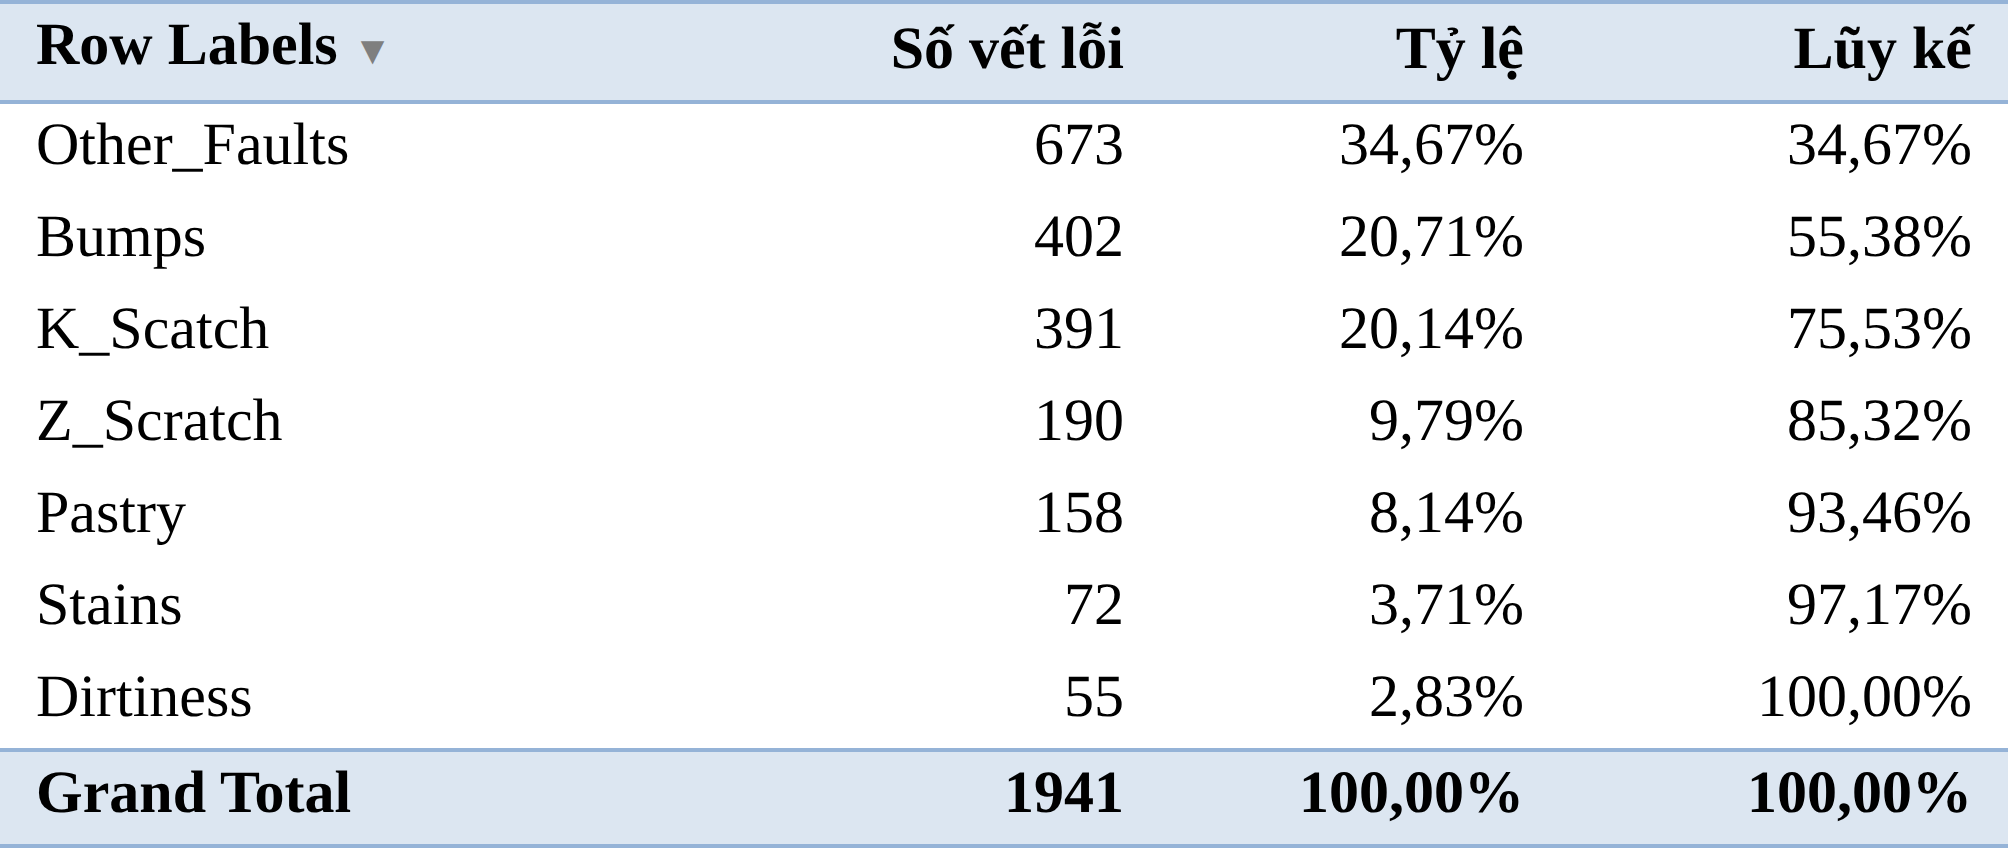
\includegraphics[width=1.0\linewidth]{Figures/fig01_bang_loi.png}
            %\begin{figurecaptionmodern}
            \capfig{Bảng Pivot tổng quan cơ cấu lỗi.}
            %\end{figurecaptionmodern}
        \end{figure}
    \end{minipage}
    &
    \justifying \noindent Hình 3 mô tả bảng Pivot tổng quan cơ cấu lỗi trên 1.941 bản ghi đã loại trùng. Ba nhóm lỗi lớn nhất (Other\_Faults, Bumps, K\_Scatch) cộng lại chiếm 75,53\% tổng số vết lỗi. Dữ liệu mất cân bằng rõ rệt ngay từ phép đếm đầu tiên.
\end{tabular}
\end{table}



\begin{notebox}[title=\faInfoCircle~\textbf{Lịch sử phiên bản số liệu}]
Các bản phân tích trước của báo cáo đều dùng đúng 1.941 bản ghi đã loại trùng. Ở giai đoạn hoàn thiện màu sắc và bố cục Dashboard, một vùng nguồn Pivot còn sót lại một bản ghi \texttt{Z\_Scratch} trên thép A400 bị nhân đôi, nên vài ảnh chụp trong các bản nháp trước hiển thị Grand Total 1.942 và \texttt{Z\_Scratch} 191 vết. Sai lệch đó chỉ nằm ở lớp trình bày và không làm thay đổi logic hoặc kết luận của báo cáo. Các bảng và biểu đồ chịu ảnh hưởng đã được tái xuất từ đúng nguồn 1.941 bản ghi trước khi đưa vào bản này.
\end{notebox}

\noindent
\textbf{Bước 3. Dựng Pivot chéo loại lỗi $\times$ dòng thép và vẽ biểu đồ}

Để trả lời Q2, dựng thêm một Pivot Table thứ hai đặt cạnh bảng trên.

\begin{enumerate}
  \item Vùng Rows nhận Fault\_Type\_Clean, vùng Columns nhận SteelType, vùng Values nhận Count of Fault\_Type\_Clean.
  \item Chọn Pivot Table vừa tạo → PivotTable Analyze → PivotChart.
  \item Chọn Column → Clustered Column → OK.
  \item Đặt tiêu đề biểu đồ \texttt{Số vết lỗi theo loại lỗi và dòng thép}.
  \item Đổi tên trục tung thành \texttt{Số vết lỗi}, giữ trục hoành là loại lỗi.
  \item Giữ Legend hiển thị hai dòng thép A300 và A400, chỉnh màu sắc và sắp xếp loại lỗi theo số lượng giảm dần cho dễ quan sát.
\end{enumerate}

% Hinh nay da duoc dung lai tu workbook 1.941 ban ghi (nguon: figures_src/build_charts.py).

\begin{table}[H]
\centering
\begin{tabular}{@{}m{0.67\linewidth} m{0.3\linewidth}@{}}
    \begin{minipage}{\linewidth}
        \vspace{-4em}
        \begin{figure}[H]
            \centering
            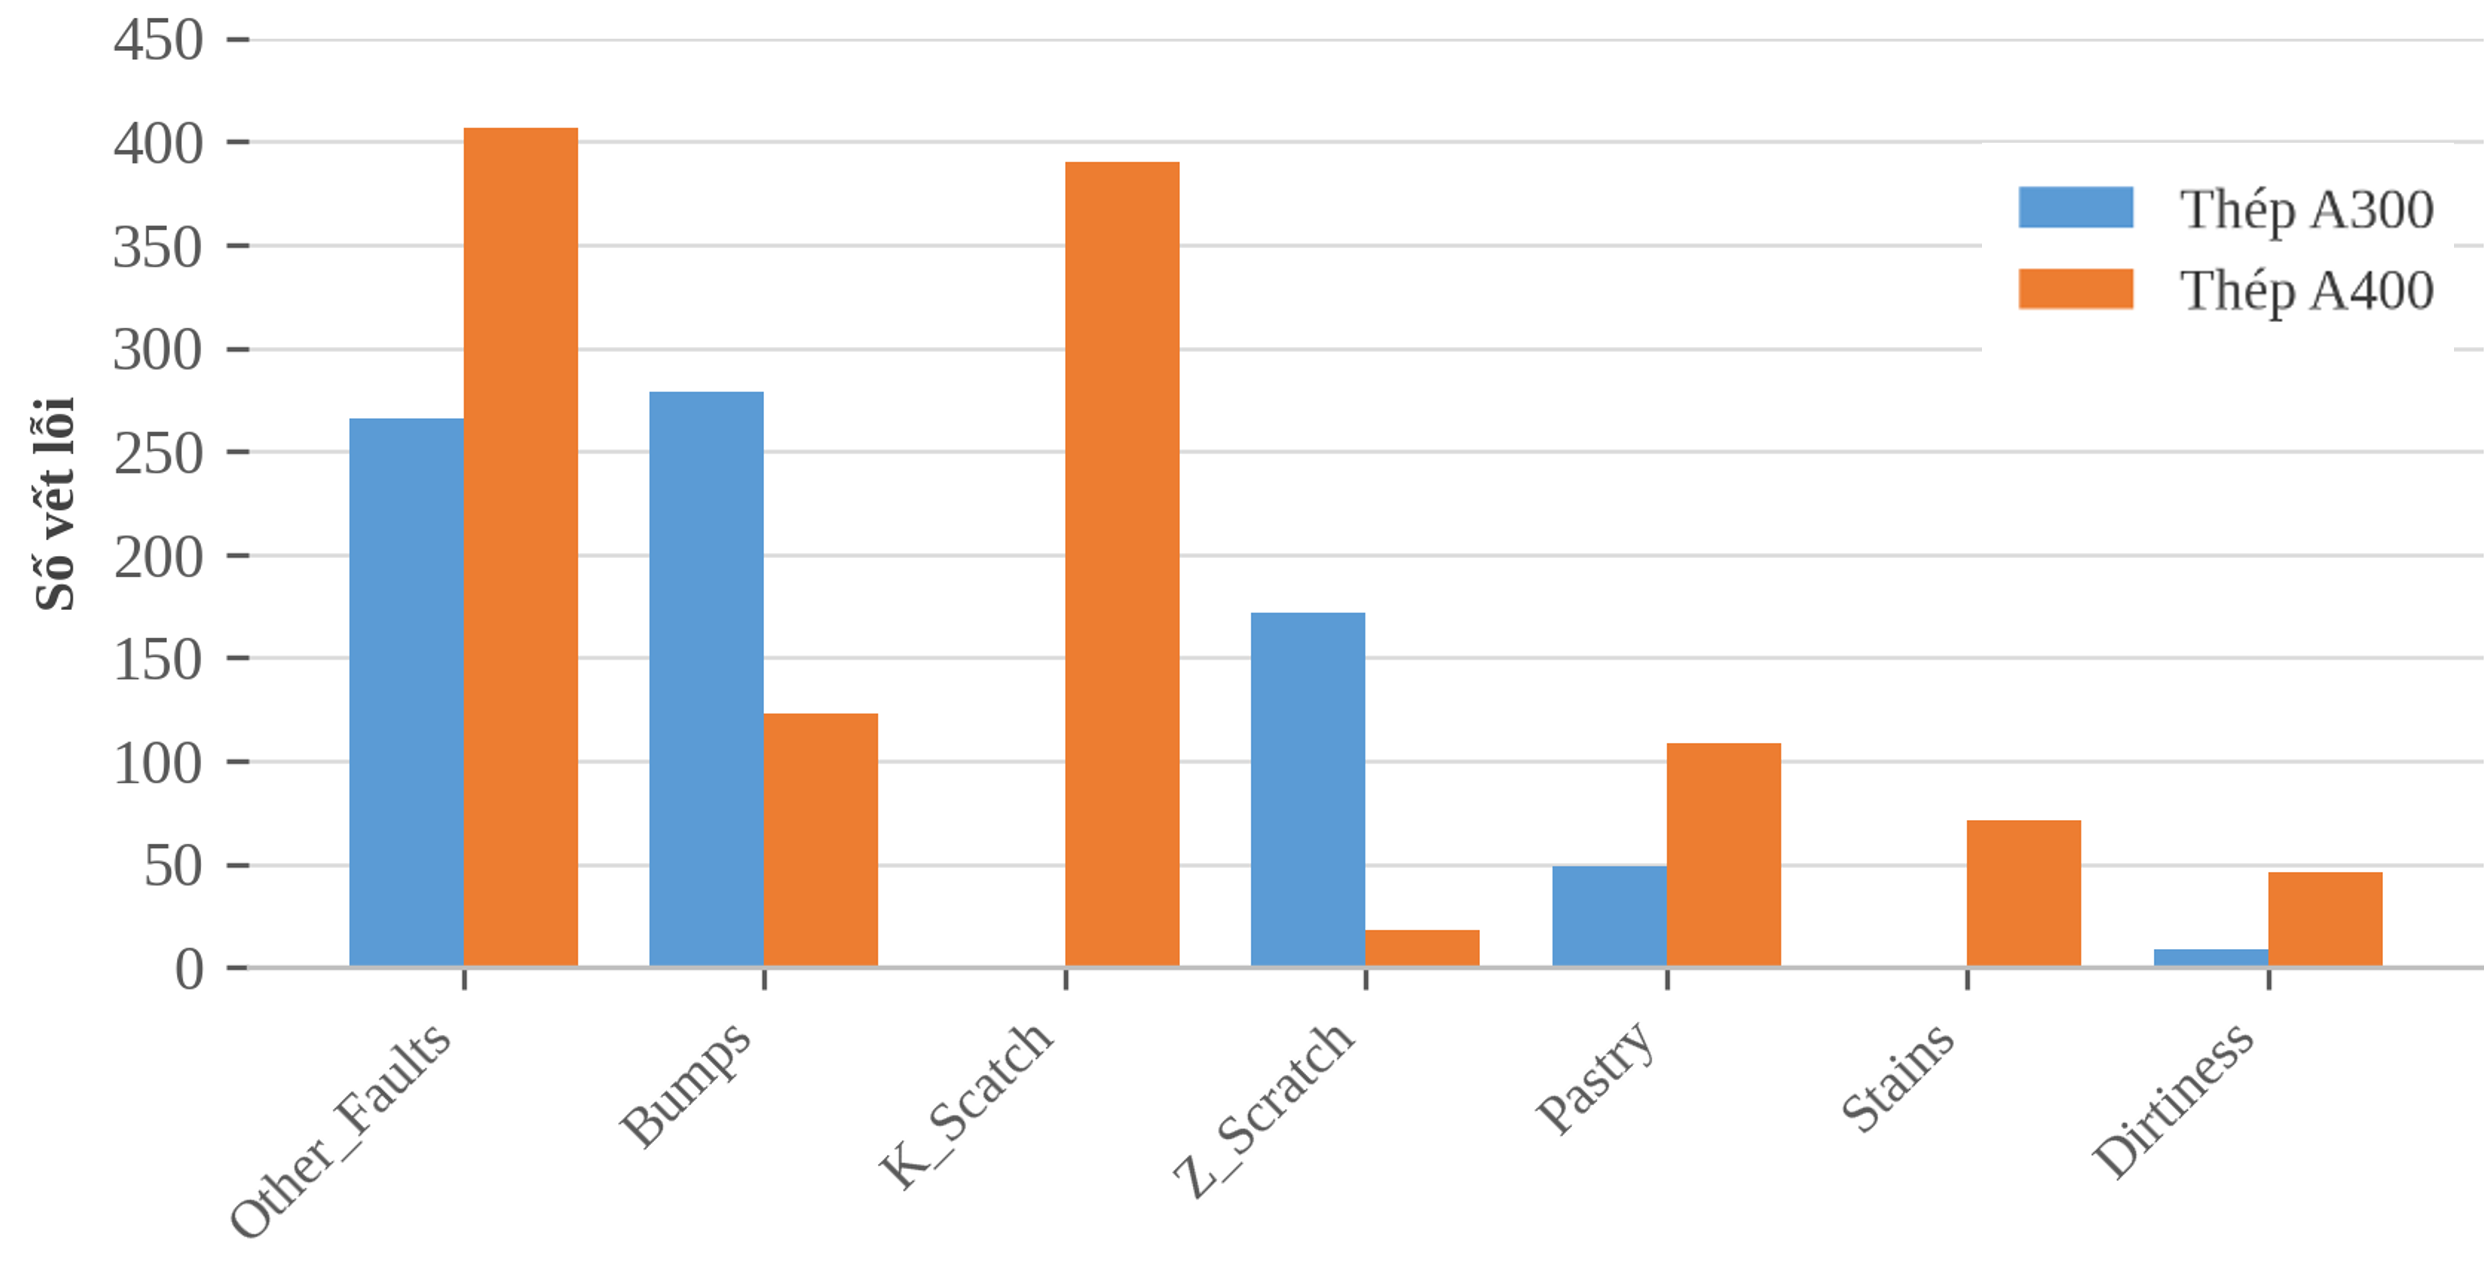
\includegraphics[width=1.0\linewidth]{Figures/fig02_bang_so_luong_loi.png}
            %\begin{figurecaptionmodern}
            \capfig{Số vết lỗi theo loại lỗi và dòng thép.}
            %\end{figurecaptionmodern}
        \end{figure}
    \end{minipage}
    &
    \justifying \noindent Hình 4 trình bày số vết lỗi theo loại lỗi và dòng thép, trên 1.941 bản ghi. K\_Scatch gần như chỉ xuất hiện trên thép A400 (390 trên 391 vết), ngược lại Z\_Scratch tập trung trên thép A300 (172 trên 190 vết). Tổng theo dòng thép là A300 777 và A400 1.164.
\end{tabular}
\end{table}



\noindent
\textbf{Bước 4. Đọc nhận định để trả lời Q1 và Q2}

\begin{itemize}
    \item \textbf{Trả lời Q1: Cơ cấu lỗi mất cân bằng rõ rệt.} Ba loại lỗi đứng đầu (Other\_Faults, Bumps và K\_Scatch) gộp lại đã là 1.466 trên 1.941 vết, chiếm 75,53\% toàn bộ dữ liệu. Bốn loại còn lại chia nhau chưa tới một phần tư, trong đó Dirtiness chỉ có 55 vết, bằng khoảng một phần mười hai nhóm lớn nhất. Mức mất cân bằng này có một hệ quả thực dụng. Nếu về sau dữ liệu được dùng để huấn luyện mô hình phân loại, một mô hình luôn gán nhãn Other\_Faults cho mọi dòng đã đạt độ chính xác (accuracy) 34,67\% mà không học được gì. Khi đó accuracy trở thành chỉ số gây hiểu lầm và phải thay bằng F1 tính theo từng lớp hoặc trung bình macro.

    \item \textbf{Other\_Faults không phải một loại lỗi.} Nhóm chiếm tỷ trọng lớn nhất lại chính là nhóm gộp các trường hợp còn lại, gồm 673 vết không có đặc trưng chung nào, như đã cảnh báo ở Mục III. Điều này giải thích vì sao các chỉ số của Other\_Faults ở những phân tích sau đều nằm quanh mức trung bình chung. Con số của nhóm là trung bình của nhiều hiện tượng khác nhau cộng lại. Muốn cơ cấu lỗi phản ánh đúng thực tế sản xuất, nhóm này cần được tách nhỏ; nội dung này sẽ được trình bày lại ở phần Khuyến nghị.

    \item \textbf{Trả lời Q2: Hai loại xước gắn với hai dòng thép gần như loại trừ nhau.} K\_Scatch có 390 trên 391 vết nằm trên thép A400 (99,74\%); Z\_Scratch ngược lại, 172 trên 190 vết nằm trên thép A300 (90,53\%). Cả hai đều vượt xa ngưỡng phán quyết 90\% đã đặt trước ở Mục V, nên kết luận có phân tách theo dòng thép được xác nhận. Stains cũng theo khuôn tương tự với 71 trên 72 vết nằm trên thép A400. Đây là mức tập trung rất cao, và nó cho biết \emph{ở đâu} có khuôn, chứ chưa cho biết \emph{vì sao}. Hai nhãn cùng mang tên vết xước lại gắn với hai dòng thép gần như loại trừ nhau là một quan sát đáng mang ra hiện trường, nhưng bảng dữ liệu không chứa biến vận hành nào để nói tiếp về cơ chế. Mức độ tập trung này sẽ còn rõ hơn khi xét thêm chiều độ dày ở Mục VII.3.

\end{itemize}

\subsection{Phân tích tương quan độ sáng của vết lỗi}
Mục này trả lời câu hỏi Q3, tức là \emph{các đặc trưng độ sáng có tách được các loại lỗi thành những vùng riêng biệt không?} Hai biến được xét là độ sáng nhỏ nhất (Minimum\_of\_Luminosity) và độ sáng lớn nhất (Maximum\_of\_Luminosity) của từng vết lỗi. Như đã phân tích ở Mục III, đây không phải thuộc tính phụ mà là tín hiệu gốc của hệ thống camera, nên nếu chúng phân tách được các loại lỗi thì khả năng nhận diện tự động là có cơ sở.\medskip

\noindent
\textbf{Bước 1. Đo mức tương quan bằng hàm thống kê}

\noindent
Trước khi vẽ, cần một con số định lượng. \emph{Hệ số tương quan Pearson} ($r$) đo mức độ quan hệ tuyến tính giữa hai biến, nhận giá trị từ $-1$ (nghịch hoàn toàn) qua 0 (không có quan hệ tuyến tính) đến $+1$ (thuận hoàn toàn). Trong Excel, hệ số này tính bằng hàm CORREL.

\begin{enumerate}
  \item Tại một ô trống ngoài vùng dữ liệu (ví dụ trên sheet phân tích), nhập công thức với hai cột J (Minimum\_of\_Luminosity) và K (Maximum\_of\_Luminosity).
  \begin{aivncodebox}[Hệ số tương quan]
  \begin{lstlisting}[language=Excel]
=CORREL(J2:J1942; K2:K1942)\end{lstlisting}
  \end{aivncodebox}
  \item Kết quả thu được là $r \approx 0{,}43$.
  \begin{itemize}
    \item Về chiều, dấu dương cho biết tương quan thuận, nghĩa là vết lỗi có điểm tối nhất càng sáng thì điểm sáng nhất cũng có xu hướng sáng theo.
    \item Về độ mạnh, mức 0,43 thuộc loại tương quan trung bình. Hai biến không gần như trùng nhau (trên 0,8), nhưng cũng không độc lập với nhau (dưới 0,2).
  \end{itemize}
\end{enumerate}

\noindent
Một hệ số đơn lẻ như $r = 0{,}43$ chỉ tóm tắt được xu hướng chung và không cho biết dữ liệu \emph{phân bố thành hình gì}. Cùng một hệ số có thể đến từ một đám mây điểm thuần nhất hoặc từ nhiều cụm tách biệt cộng lại. Với câu hỏi Q3 (vốn hỏi về \emph{các cụm theo loại lỗi}), cần nhìn thấy toàn bộ 1.941 điểm dữ liệu cùng lúc.

\noindent
Công cụ phù hợp là \emph{biểu đồ phân tán} (Scatter Plot), trong đó mỗi vết lỗi là một điểm trên hệ trục (Min, Max). Khi gán màu theo 7 loại lỗi, biểu đồ này cho phép.
\begin{itemize}
  \item Nhận ra các dải giới hạn quang học đặc thù của bề mặt thép (như dải trần nằm ngang ở mức độ sáng từ 120 đến 150 sẽ thấy ở phần đọc kết quả).
  \item Khoanh vùng các điểm bất thường (vết lỗi chói sáng hoặc tối đen khác thường) để đội QC kiểm tra lại cảm biến.
  \item So sánh trực tiếp vùng phân bố độ sáng của từng loại lỗi, tức là trả lời Q3 bằng mắt trước khi trả lời bằng con số.
\end{itemize}

\noindent
\textbf{Bước 2. Chuẩn bị dữ liệu vẽ Scatter Plot}

\noindent
Muốn mỗi loại lỗi hiện thành một màu riêng, phải tách giá trị trục tung thành 7 cột. Mỗi cột là một chuỗi (series) của biểu đồ, và Excel yêu cầu các cột này nằm liền kề cột trục hoành. Nguyên tắc tách là giá trị Maximum\_of\_Luminosity của một dòng chỉ được điền vào cột của đúng loại lỗi dòng đó, còn sáu cột kia nhận mã \#N/A.

\noindent
Lý do phải dùng \#N/A thay cho ô rỗng hoặc số 0 nằm ở cách Excel dựng biểu đồ. Excel coi chuỗi rỗng ("") và số 0 là tọa độ thật nên sẽ vẽ đè hàng loạt điểm xuống đáy biểu đồ, riêng ô chứa \#N/A thì bị bỏ qua hoàn toàn. Nhờ vậy mỗi điểm chỉ xuất hiện đúng một lần, ở đúng chuỗi màu của nó.

\begin{enumerate}
  \item Copy cột Minimum\_of\_Luminosity sang cột AM (làm cột trục hoành).
  \item Tại 7 cột tiếp theo (AN đến AT), gõ tiêu đề của 7 loại lỗi lên dòng 1, lần lượt là Pastry, Z\_Scratch, K\_Scatch, Stains, Dirtiness, Bumps, Other\_Faults.
  \item Tại ô AN2 (ngay dưới tiêu đề Pastry), nhập công thức \texttt{=IF(\$AD2=AN\$1; \$K2; NA())} nhằm đối chiếu nhãn đã làm sạch ở cột AD với tiêu đề cột và lấy giá trị Max từ cột K khi khớp.
  \item Kéo công thức từ AN2 sang ngang đến AT2.
  \item Bôi đen AN2:AT2 rồi nhấp đúp vào góc dưới bên phải vùng chọn để công thức tự chạy xuống hết 1.941 dòng dữ liệu.
  \item Kiểm tra lại, trên mỗi dòng chỉ có đúng một cột hiện số, sáu cột còn lại hiển thị \#N/A.
  \item Bôi đen toàn bộ vùng 8 cột vừa dựng (AM1:AT1942) bằng cách chọn AM1:AT1, sau đó nhấn Ctrl + Shift + Mũi tên xuống.
\end{enumerate}

\noindent
\textbf{Bước 3. Chèn biểu đồ Scatter Plot}

\begin{enumerate}
  \item Trên thanh Ribbon, chọn thẻ Insert.
  \item Trong nhóm Charts, click biểu tượng các dấu chấm rải rác (Insert Scatter (X, Y) or Bubble Chart).
  \item Chọn loại Scatter cơ bản (chỉ có điểm, không có đường nối).
  \item Excel dựng một biểu đồ với 1.941 dấu chấm, mỗi chấm tương ứng với một vết lỗi.
\end{enumerate}

\noindent
\textbf{Bước 4. Tùy biến biểu đồ}

Biểu đồ mặc định của Excel cần định dạng lại trước khi đưa vào báo cáo.

\begin{enumerate}
  \item Thêm tiêu đề trục (Axis Titles) theo hai bước.
  \begin{itemize}
    \item Click vào biểu đồ, nhấn dấu [+] ở góc phải (Chart Elements), tích chọn Axis Titles.
    \item Đặt tên trục X (nằm ngang) là Minimum Luminosity, trục Y (thẳng đứng) là Maximum Luminosity.
  \end{itemize}
  \item Làm mờ các điểm để tránh hiện tượng vẽ đè (overplotting).
  \begin{itemize}
    \item 1.941 điểm đè lên nhau khiến mật độ khó quan sát nếu để màu đặc.
    \item Click đúp vào một dấu chấm bất kỳ; ở khung bên phải chọn biểu tượng thùng sơn (Fill \& Line) → Marker → Fill.
    \item Chọn Solid fill, chọn màu, rồi kéo thanh Transparency lên mức 60 đến 70\%. Những vùng nhiều vết lỗi chồng lên nhau sẽ tự hiện đậm hơn, làm nổi rõ các cụm (cluster).
  \end{itemize}

\end{enumerate}

% Hinh nay da duoc dung lai tu workbook 1.941 ban ghi (nguon: figures_src/build_charts.py).


\begin{table}[H]
\centering
\begin{tabular}{@{}m{0.67\linewidth} m{0.3\linewidth}@{}}
    \begin{minipage}{\linewidth}
        \vspace{-4em}
        \begin{figure}[H]
            \centering
            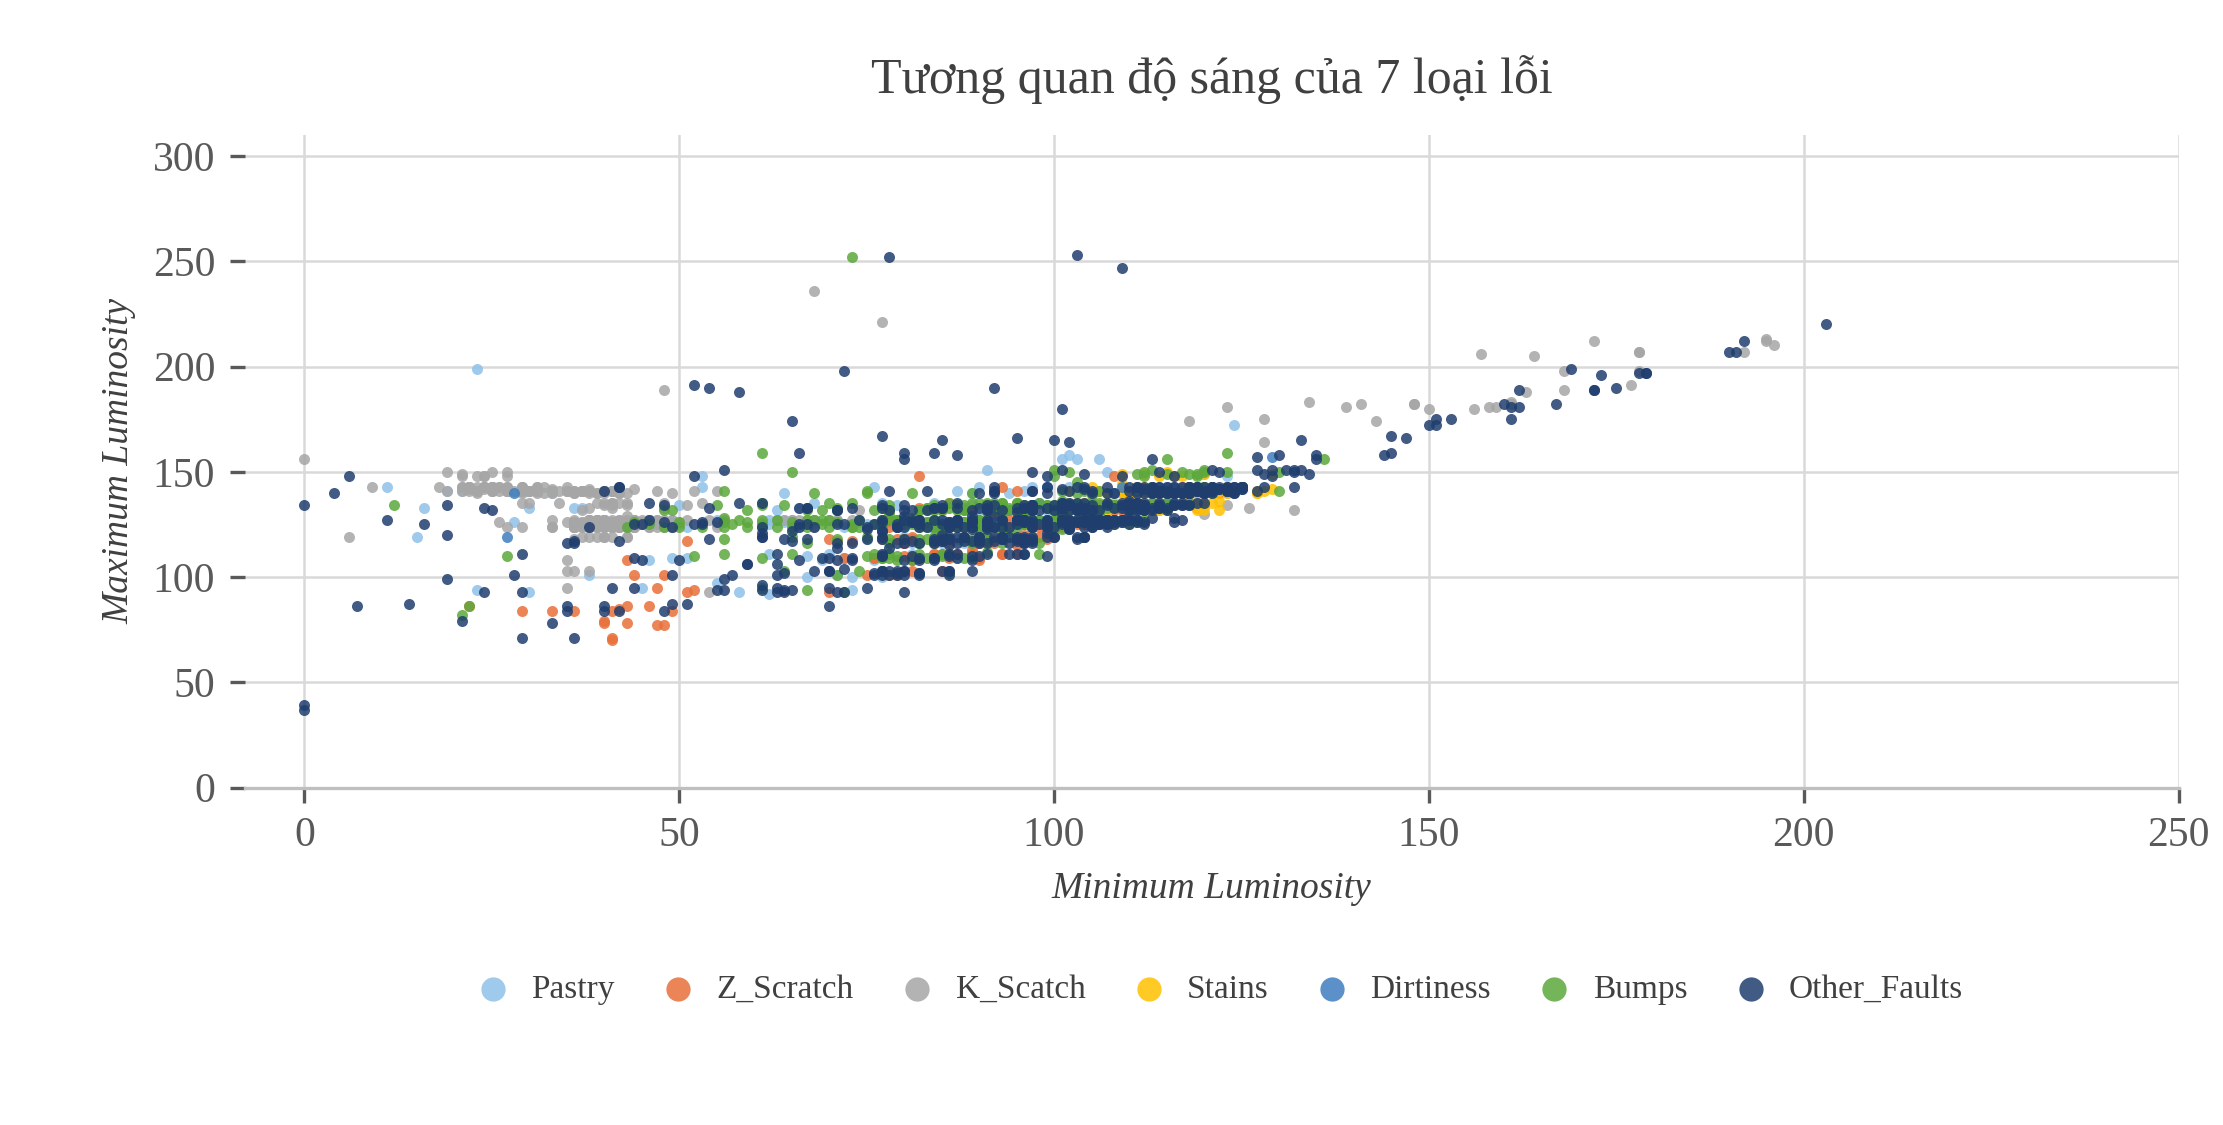
\includegraphics[width=1.0\linewidth]{Figures/fig03_bang_scatterplot.png}
            %\begin{figurecaptionmodern}
            \capfig{Biểu đồ phân tán độ sáng Min và Max theo bảy loại lỗi.}
            %\end{figurecaptionmodern}
        \end{figure}
    \end{minipage}
    &
    \justifying \noindent Hình 5 trình bày biểu đồ phân tán độ sáng Min và Max theo bảy loại lỗi, $n = 1.941$, Pearson $r = 0{,}4296$. Mỗi loại lỗi chiếm một vùng độ sáng tương đối riêng; nổi bật nhất là cụm K\_Scatch dồn về phía trái, nơi độ sáng tối thiểu thấp nhất trong bảy nhãn.
\end{tabular}
\end{table}




\noindent
\textbf{Bước 5. Đọc nhận định để trả lời Q3}

\begin{enumerate}
  \item \textbf{K\_Scatch chiếm một vùng riêng ở phía độ sáng tối thiểu thấp.} Trung vị \texttt{Minimum\_of\_Luminosity} của K\_Scatch là 41, trong khi trung vị của năm nhãn còn lại nằm trong khoảng 80 đến 97. Có 297 trên 391 bản ghi K\_Scatch (76,0\%) mang giá trị dưới 50, còn trung vị \texttt{Maximum\_of\_Luminosity} của nhãn này là 134, không thấp hơn các nhãn khác. Nói cách khác, K\_Scatch tách khỏi phần còn lại chủ yếu ở \emph{một chiều duy nhất}, là chiều độ sáng tối thiểu.

  \item \textbf{Z\_Scratch có độ sáng tối đa thấp nhất, nhưng khoảng cách rất nhỏ.} Trung vị \texttt{Maximum\_of\_Luminosity} của Z\_Scratch là 124, so với 126 của Pastry, 127 của Bumps và 127 của Other\_Faults. Đây đúng là giá trị thấp nhất trong nhóm, nhưng chênh lệch chỉ khoảng ba đơn vị trên một thang trải từ 38 đến 253. Chênh lệch ở mức đó không đủ để tách Z\_Scratch bằng một ngưỡng trên trục này, và báo cáo không rút ra kết luận nào từ nó.

  \item \textbf{Ở vùng độ sáng nền cao, hiệu Max $-$ Min gần như là một hằng số.} Xét 140 bản ghi có Min $>$ 120, hiệu Max $-$ Min có trung vị 19 và khoảng tứ phân vị từ 17 đến 23. Trên biểu đồ, các điểm này xếp thành một đường chéo dốc lên gần như thẳng, khác hẳn vùng phân tán không có hướng rõ ràng ở khu vực trung tâm. Other\_Faults chiếm 74 trên 140 bản ghi của vùng này. Một nhóm con có quan hệ chặt đến vậy nằm lẫn trong nhãn gộp là thêm một lý do để tách nhỏ Other\_Faults, và tách bằng chính hai biến độ sáng này là một hướng thử được.

  \item \textbf{Trục Max có một dải tập trung trong khoảng từ 120 đến 150, và dải này là đặc điểm chung của cả bộ dữ liệu.} Có 1.432 trên 1.941 bản ghi (73,8\%) mang \texttt{Maximum\_of\_Luminosity} trong khoảng này. Tỷ lệ của Bumps là 80,8\% và của Pastry là 69,0\%, tức là dao động quanh mức chung chứ không phải đặc trưng riêng của hai nhãn đó. Báo cáo dừng ở mô tả này. Giải thích vì sao trục Max lại dồn vào một dải hẹp đòi hỏi biết cách hệ thống đo được hiệu chỉnh, và không có tài liệu nào cho phép nói tiếp.

\end{enumerate}

\noindent
\textbf{Bước 6. Thử một quy tắc nhận diện và đo nó}

\noindent
Cụm K\_Scatch tách đủ rõ để thử một quy tắc ngưỡng. Dùng \texttt{COUNTIFS} ngay trên bảng dữ liệu với điều kiện Min $<$ 50 và Max $>$ 120, quy tắc gắn cờ 325 bản ghi, trong đó 282 bản ghi đúng là K\_Scatch.

\begin{center}
\small
\begin{tabular}{@{}p{4.6cm} r p{9.0cm}@{}}
\toprule
\textbf{Chỉ tiêu} & \textbf{Giá trị} & \textbf{Cách đọc} \\
\midrule
Số bản ghi bị gắn cờ & 325 & Toàn bộ dự báo dương của quy tắc \\
Trong đó đúng K\_Scatch & 282 & Dự báo dương đúng \\
Precision & 86,77\% & 282 trên 325 bản ghi bị gắn cờ là K\_Scatch thật \\
Recall & 72,12\% & 282 trên 391 bản ghi K\_Scatch bị quy tắc bắt được \\
\bottomrule
\end{tabular}
\end{center}

\noindent
Hai con số này \textbf{không phải accuracy}, và cũng chưa phải hiệu năng của quy tắc. Chúng được tính trên đúng bộ dữ liệu đã dùng để chọn ra hai ngưỡng 50 và 120, nên chắc chắn lạc quan hơn thực tế. Muốn biết quy tắc chạy được đến đâu, phải đo lại trên một tập kiểm tra độc lập chưa từng tham gia vào việc chọn ngưỡng. Đây là việc đặt ở Giai đoạn 3 của Mục X.

\noindent
Tóm lại, câu trả lời cho Q3 là \textbf{có, nhưng chỉ với một nhãn}. K\_Scatch chiếm một vùng độ sáng tách được bằng ngưỡng, và một quy tắc hai điều kiện đã bắt được phần lớn nhóm này. Sáu nhãn còn lại chồng lấn nhau trên cả hai trục độ sáng, nên với chúng, độ sáng chưa đủ để nhận diện.

\subsection{Phân tích ảnh hưởng của độ dày tấm thép}
Mục này trả lời câu hỏi Q4, tức là \emph{độ dày tấm thép có liên quan tới loại lỗi hay không?} Về mặt vật lý, độ dày ảnh hưởng trực tiếp đến điều kiện cán. Tấm mỏng và tấm dày khác nhau về truyền nhiệt, áp lực cán và khả năng chịu biến dạng, nên hoàn toàn có thể khác nhau về nguy cơ phát sinh từng loại lỗi. Phân tích đi theo ba lớp, từ tổng thể đến chi tiết, lần lượt là phân bố độ dày của toàn bộ vết lỗi, độ dày đặc trưng của từng loại lỗi, và cuối cùng là độ dày theo từng loại lỗi trên từng dòng thép.

\noindent
Cần nhắc lại giới hạn đã nêu ở Mục IV trước khi đọc bất kỳ con số nào dưới đây. Bảng dữ liệu chỉ chứa các vết lỗi, không chứa sản lượng. \emph{Độ dày 40 xuất hiện nhiều nhất trong các vết lỗi} chưa chứng minh tấm dày 40 dễ lỗi hơn, vì có thể nhà máy đơn giản là sản xuất loại 40 nhiều nhất.\medskip

\noindent
\textbf{Bước 1. Tính thống kê mô tả về độ dày của các tấm thép có lỗi}

\noindent
\emph{Thống kê mô tả} (descriptive statistics) là bộ chỉ số tóm tắt một cột dữ liệu, gồm trung bình, trung vị, độ lệch chuẩn, giá trị nhỏ nhất/lớn nhất\ldots{} Excel tính sẵn cả bộ qua công cụ Data Analysis ToolPak.

\begin{enumerate}
  \item Chọn tab Data → Data Analysis (nếu chưa thấy, bật Analysis ToolPak trong File → Options → Add-ins) → Descriptive Statistics → OK.
  \item Ở Input Range, quét vùng dữ liệu cột Steel\_Plate\_Thickness.
  \item Tích chọn Summary statistics và Labels in First Row (do vùng chọn có tiêu đề cột).
  \item Ở Output Range, chọn một ô trên sheet phân tích (ví dụ A7) → OK.
\end{enumerate}

% Hinh nay da duoc dung lai tu workbook 1.941 ban ghi (nguon: figures_src/build_tables.py). Khong can chup lai tu Excel.
\begin{figure}[H]
    \centering
    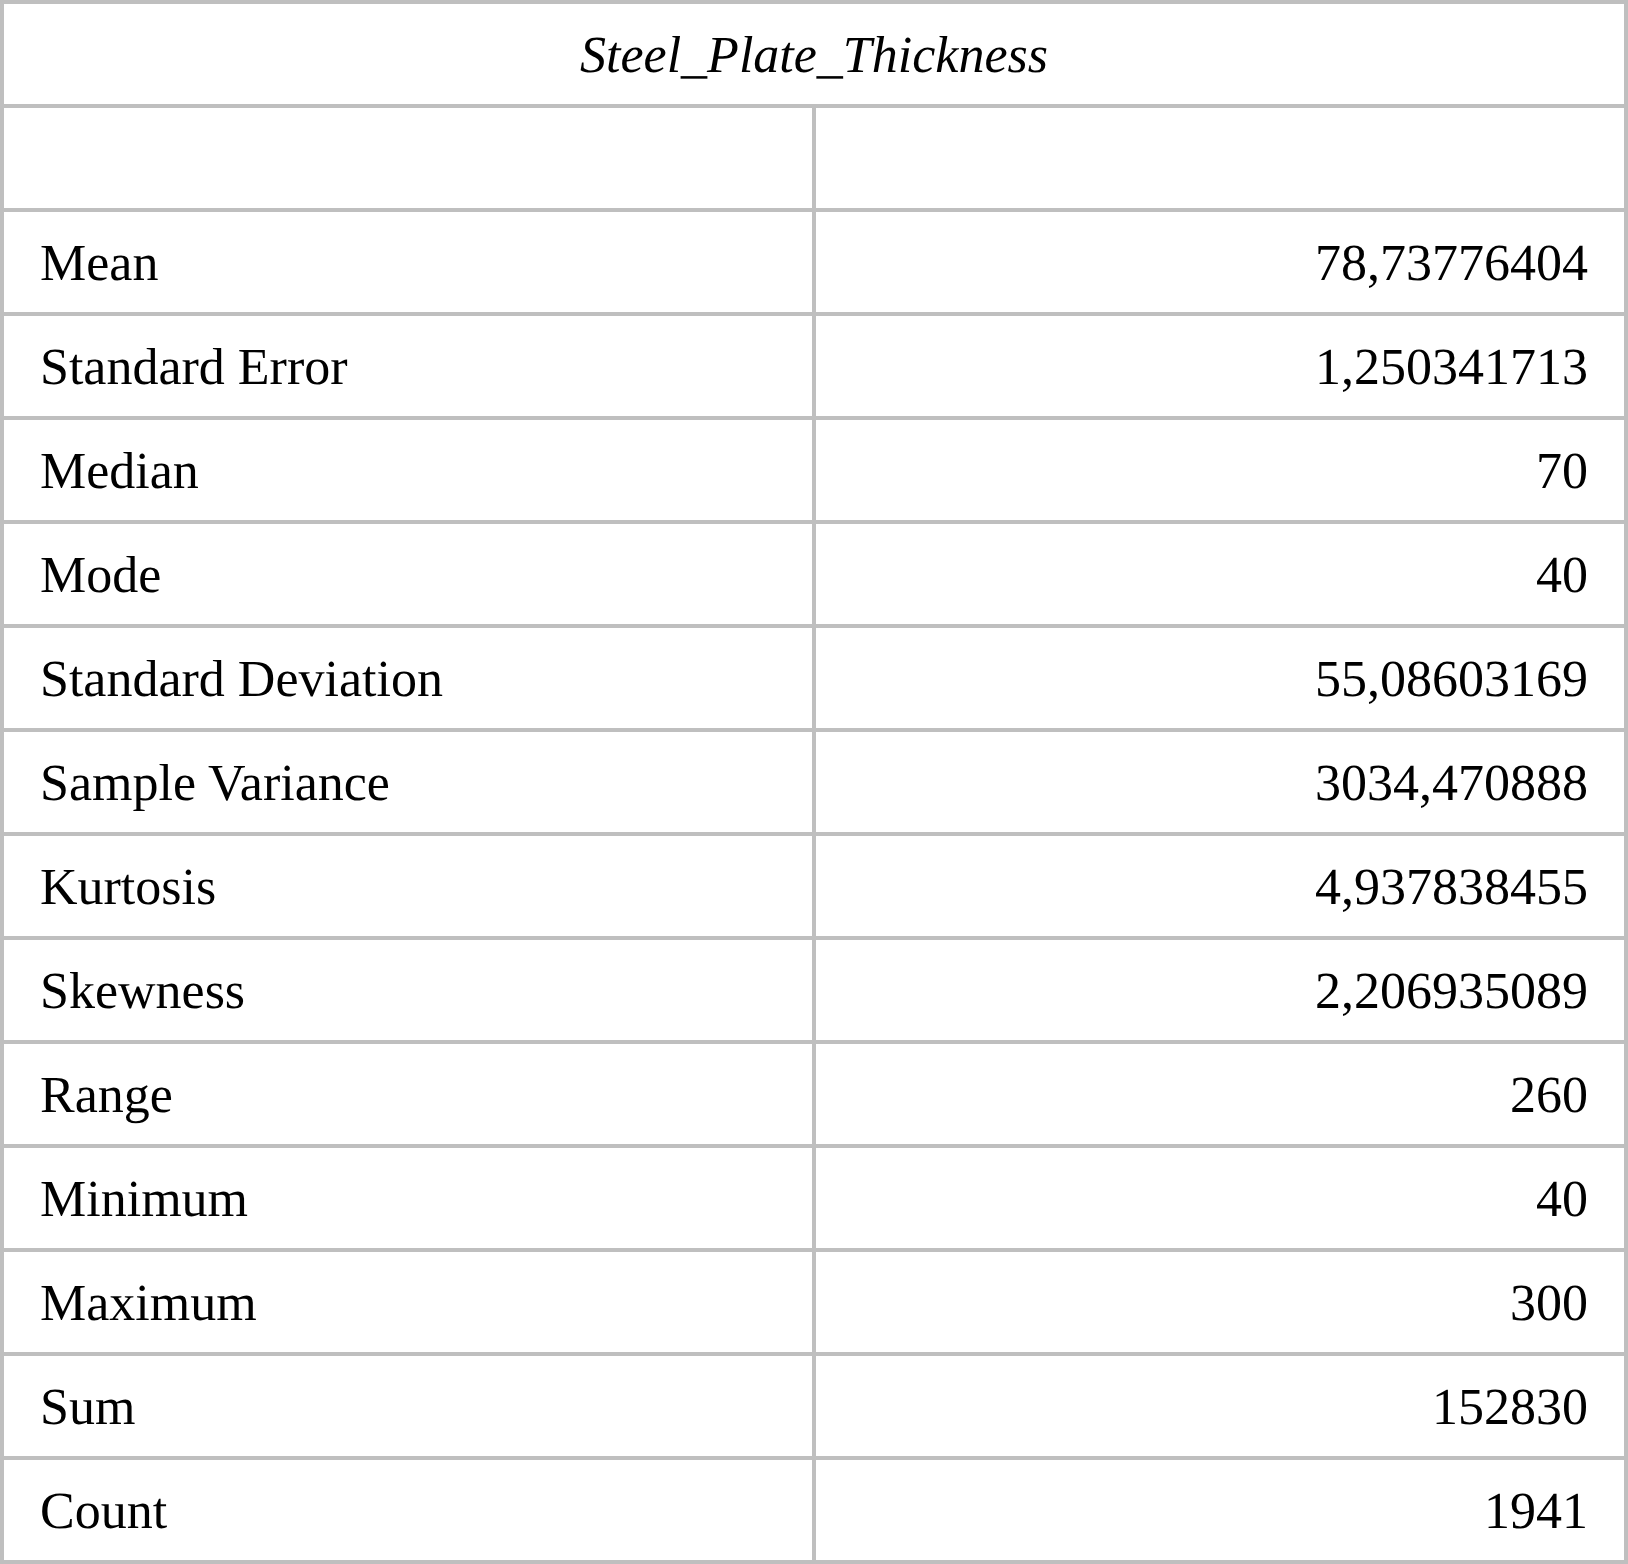
\includegraphics[width=0.5\linewidth]{Figures/fig04_thong_ke_do_day.png}
    \begin{figurecaptionmodern}
    \capfig{Thống kê mô tả độ dày tấm thép trên 1.941 bản ghi. Phân phối lệch phải mạnh, với trung vị chỉ 70 trong khi giá trị lớn nhất lên tới 300, nên trung bình bị kéo lên 78,74.}
    \end{figurecaptionmodern}
\end{figure}

\noindent
\textbf{Bước 2. Vẽ biểu đồ hộp}

\begin{enumerate}
  \item Chọn vùng dữ liệu cần vẽ (cột Steel\_Plate\_Thickness).
  \item Chọn tab Insert → Statistic Chart → Box and Whisker.
  \item Điều chỉnh và đặt tiêu đề cho biểu đồ.
\end{enumerate}

% Hinh nay da duoc dung lai tu workbook 1.941 ban ghi (nguon: figures_src/build_charts.py).

\begin{table}[H]
\centering
\begin{tabular}{@{}m{0.67\linewidth} m{0.3\linewidth}@{}}
    \begin{minipage}{\linewidth}
        \vspace{-5em}
        \begin{figure}[H]
            \centering
            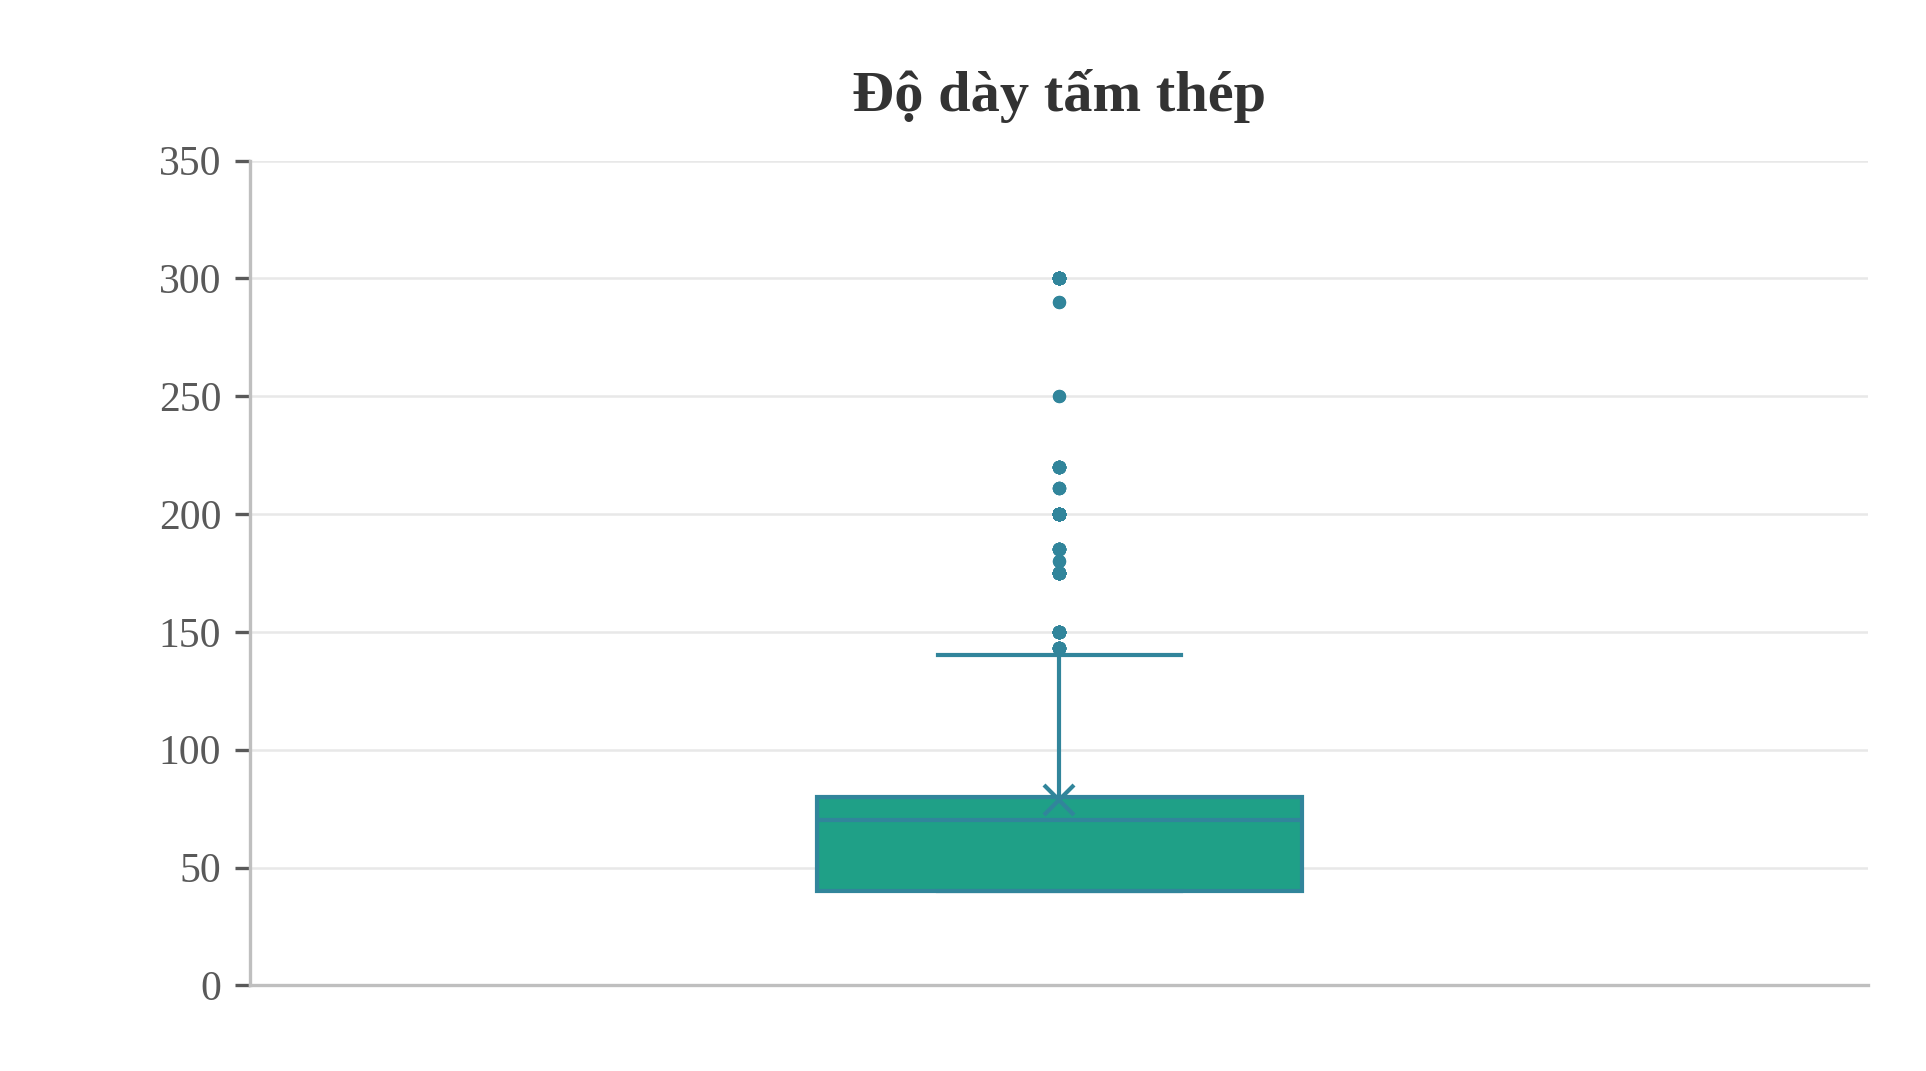
\includegraphics[width=1.0\linewidth]{Figures/fig05_boxplot.png}
            %\begin{figurecaptionmodern}
            \capfig{Biểu đồ hộp cho đặc trưng \texttt{Steel\_Plate\_Thickness}.}
            %\end{figurecaptionmodern}
        \end{figure}
    \end{minipage}
    &
    \justifying \noindent Hình 7 trình bày biểu đồ hộp \texttt{Steel\_Plate\_Thickness} trên 1.941 bản ghi. Phân bố lệch phải, với Q1 = 40, trung vị 70, Q3 = 80 và giá trị lớn nhất 300. Thân hộp dồn về phía giá trị nhỏ, đuôi trên kéo dài với nhiều điểm tách rời. Nguồn không công bố đơn vị của biến này.
\end{tabular}
\end{table}




\noindent
\textbf{Bước 3. Dựng Pivot Table độ dày theo từng loại lỗi}

\begin{enumerate}
  \item Chọn toàn bộ vùng dữ liệu.
  \item Chọn Insert → PivotTable → chọn vị trí đặt Pivot Table.
  \item Kéo thả sao cho vùng Rows nhận Fault\_Type\_Clean, còn vùng Values nhận cột Steel\_Plate\_Thickness kéo vào 3 lần.
  \item Đổi tên ba cột giá trị lần lượt thành \texttt{Số lượng lỗi}, \texttt{Độ dày trung bình}, \texttt{Độ lệch chuẩn độ dày}.
  \item Tại PivotTable Fields, nhấn vào trường \texttt{Số lượng lỗi} → Value Field Settings → Count; trường \texttt{Độ dày trung bình} → Average; trường \texttt{Độ lệch chuẩn độ dày} → StdDev.
\end{enumerate}

% Hinh nay da duoc dung lai tu workbook 1.941 ban ghi (nguon: figures_src/build_tables.py). Khong can chup lai tu Excel.

\begin{table}[H]
\centering
\begin{tabular}{@{}m{0.67\linewidth} m{0.3\linewidth}@{}}
    \begin{minipage}{\linewidth}
        \vspace{-4em}
        \begin{figure}[H]
            \centering
            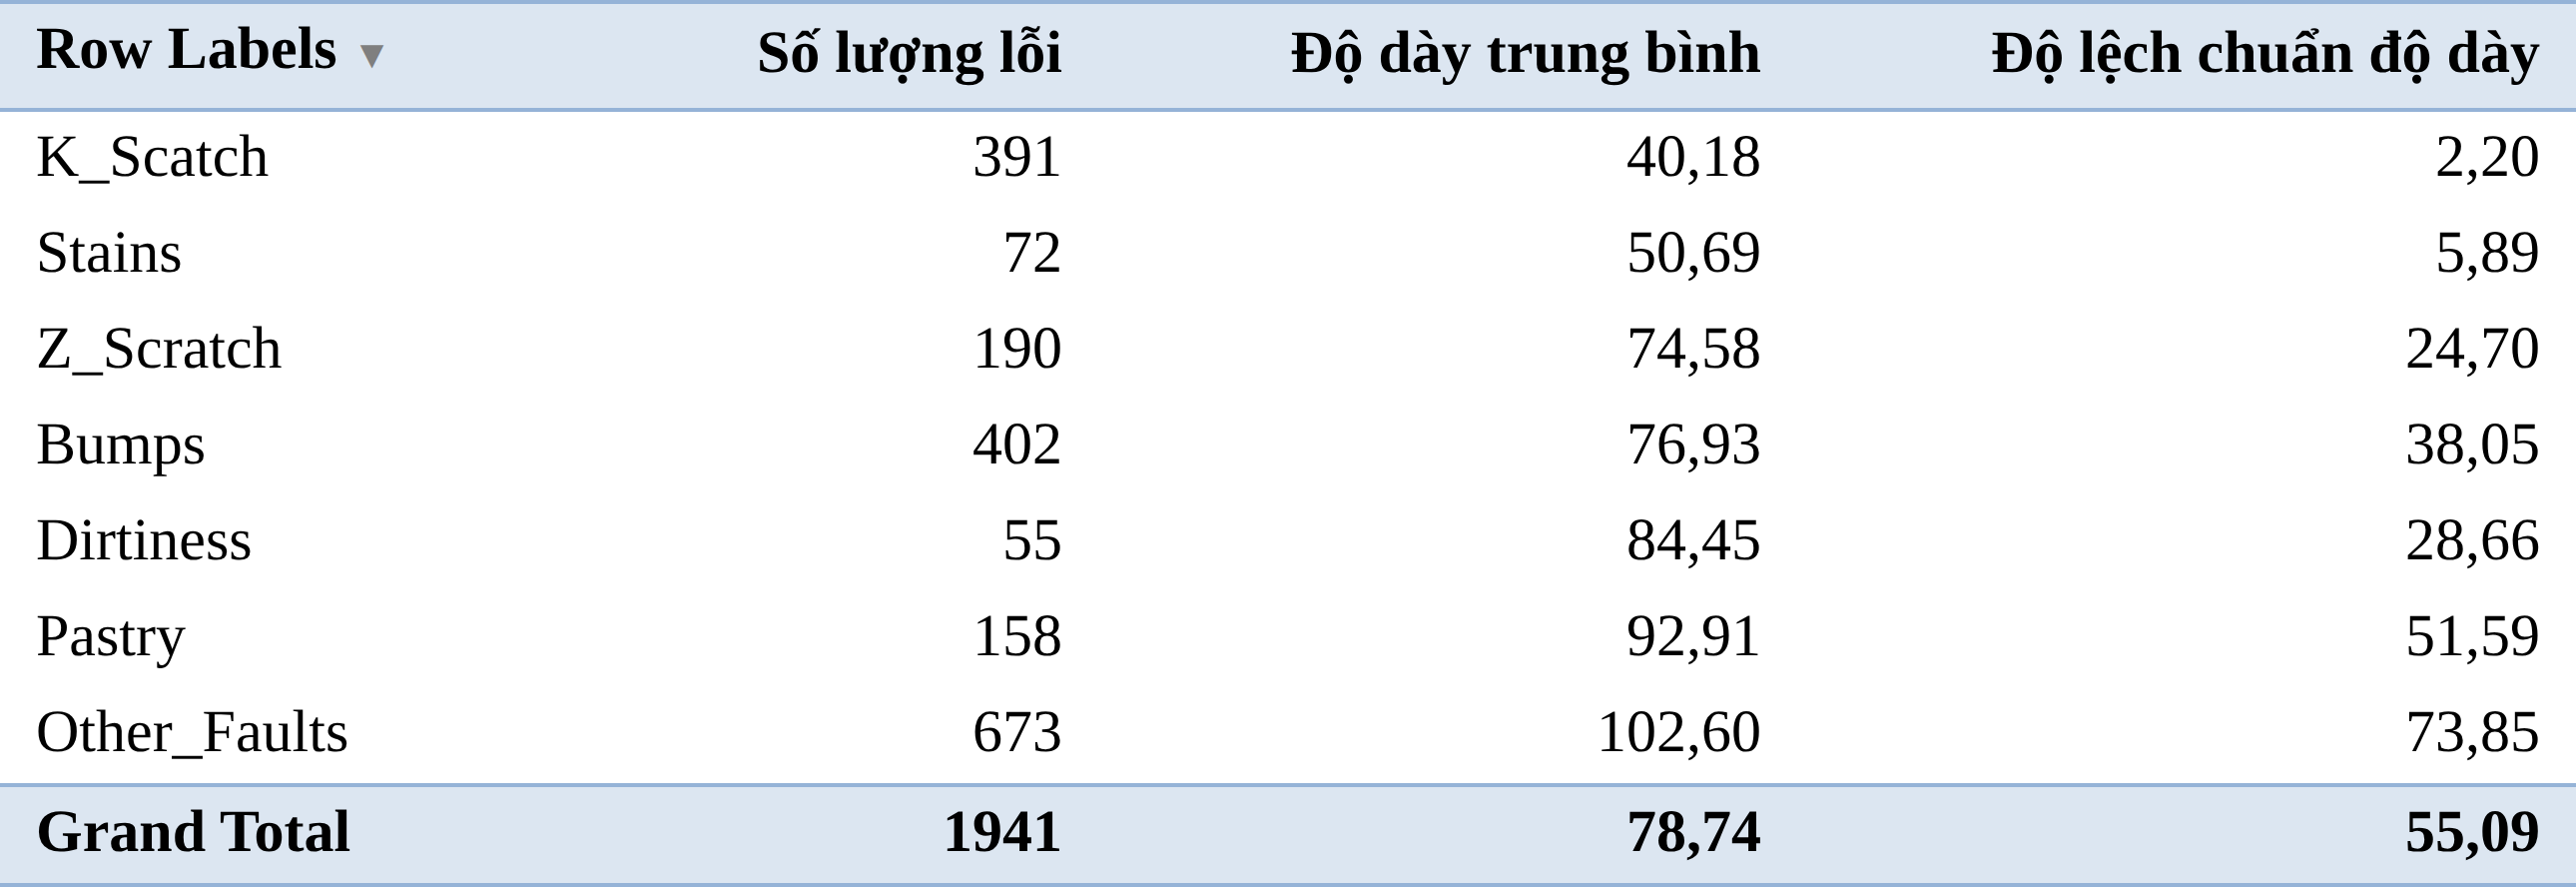
\includegraphics[width=1.0\linewidth]{Figures/fig06_bang_do_day.png}           
            \capfig{Độ dày trung bình và độ lệch chuẩn.}           
        \end{figure}
    \end{minipage}
    &
    \justifying \noindent Hình 8 mô tả độ dày trung bình và độ lệch chuẩn mẫu theo bảy loại lỗi, tính trên 1.941 bản ghi. K\_Scatch có độ lệch chuẩn nhỏ nhất (2,20), nghĩa là gần như toàn bộ vết lỗi dồn về đúng một mức độ dày 40.
\end{tabular}
\end{table}



\noindent
\textbf{Bước 4. Vẽ biểu đồ cột kèm thanh sai số}

\begin{enumerate}
  \item Dựng thêm một Pivot chỉ chứa độ dày trung bình theo từng loại lỗi.
  \item Chọn Pivot Table → PivotTable Analyze → PivotChart.
  \item Chọn biểu đồ cột (Clustered Column) → OK.
  \item Chọn biểu đồ → Design → Add Chart Element → Error Bars → Standard Deviation.
  \item Nhấp chuột phải vào Error Bars → Format Error Bar, chọn Direction là Both, End Style là Cap và Error Amount là Custom → Specify Value → quét vùng độ lệch chuẩn ở Pivot Bước 3 cho cả Positive và Negative → OK. Thanh sai số lúc này thể hiện đúng độ phân tán thật của từng loại lỗi thay vì một giá trị mặc định.
  \item Điều chỉnh và đặt tiêu đề cho biểu đồ.
\end{enumerate}

% Hinh nay da duoc dung lai tu workbook 1.941 ban ghi (nguon: figures_src/build_charts.py).

\begin{table}[H]
\centering
\begin{tabular}{@{}m{0.67\linewidth} m{0.3\linewidth}@{}}
    \begin{minipage}{\linewidth}
        \vspace{-5em}
        \begin{figure}[H]
            \centering
            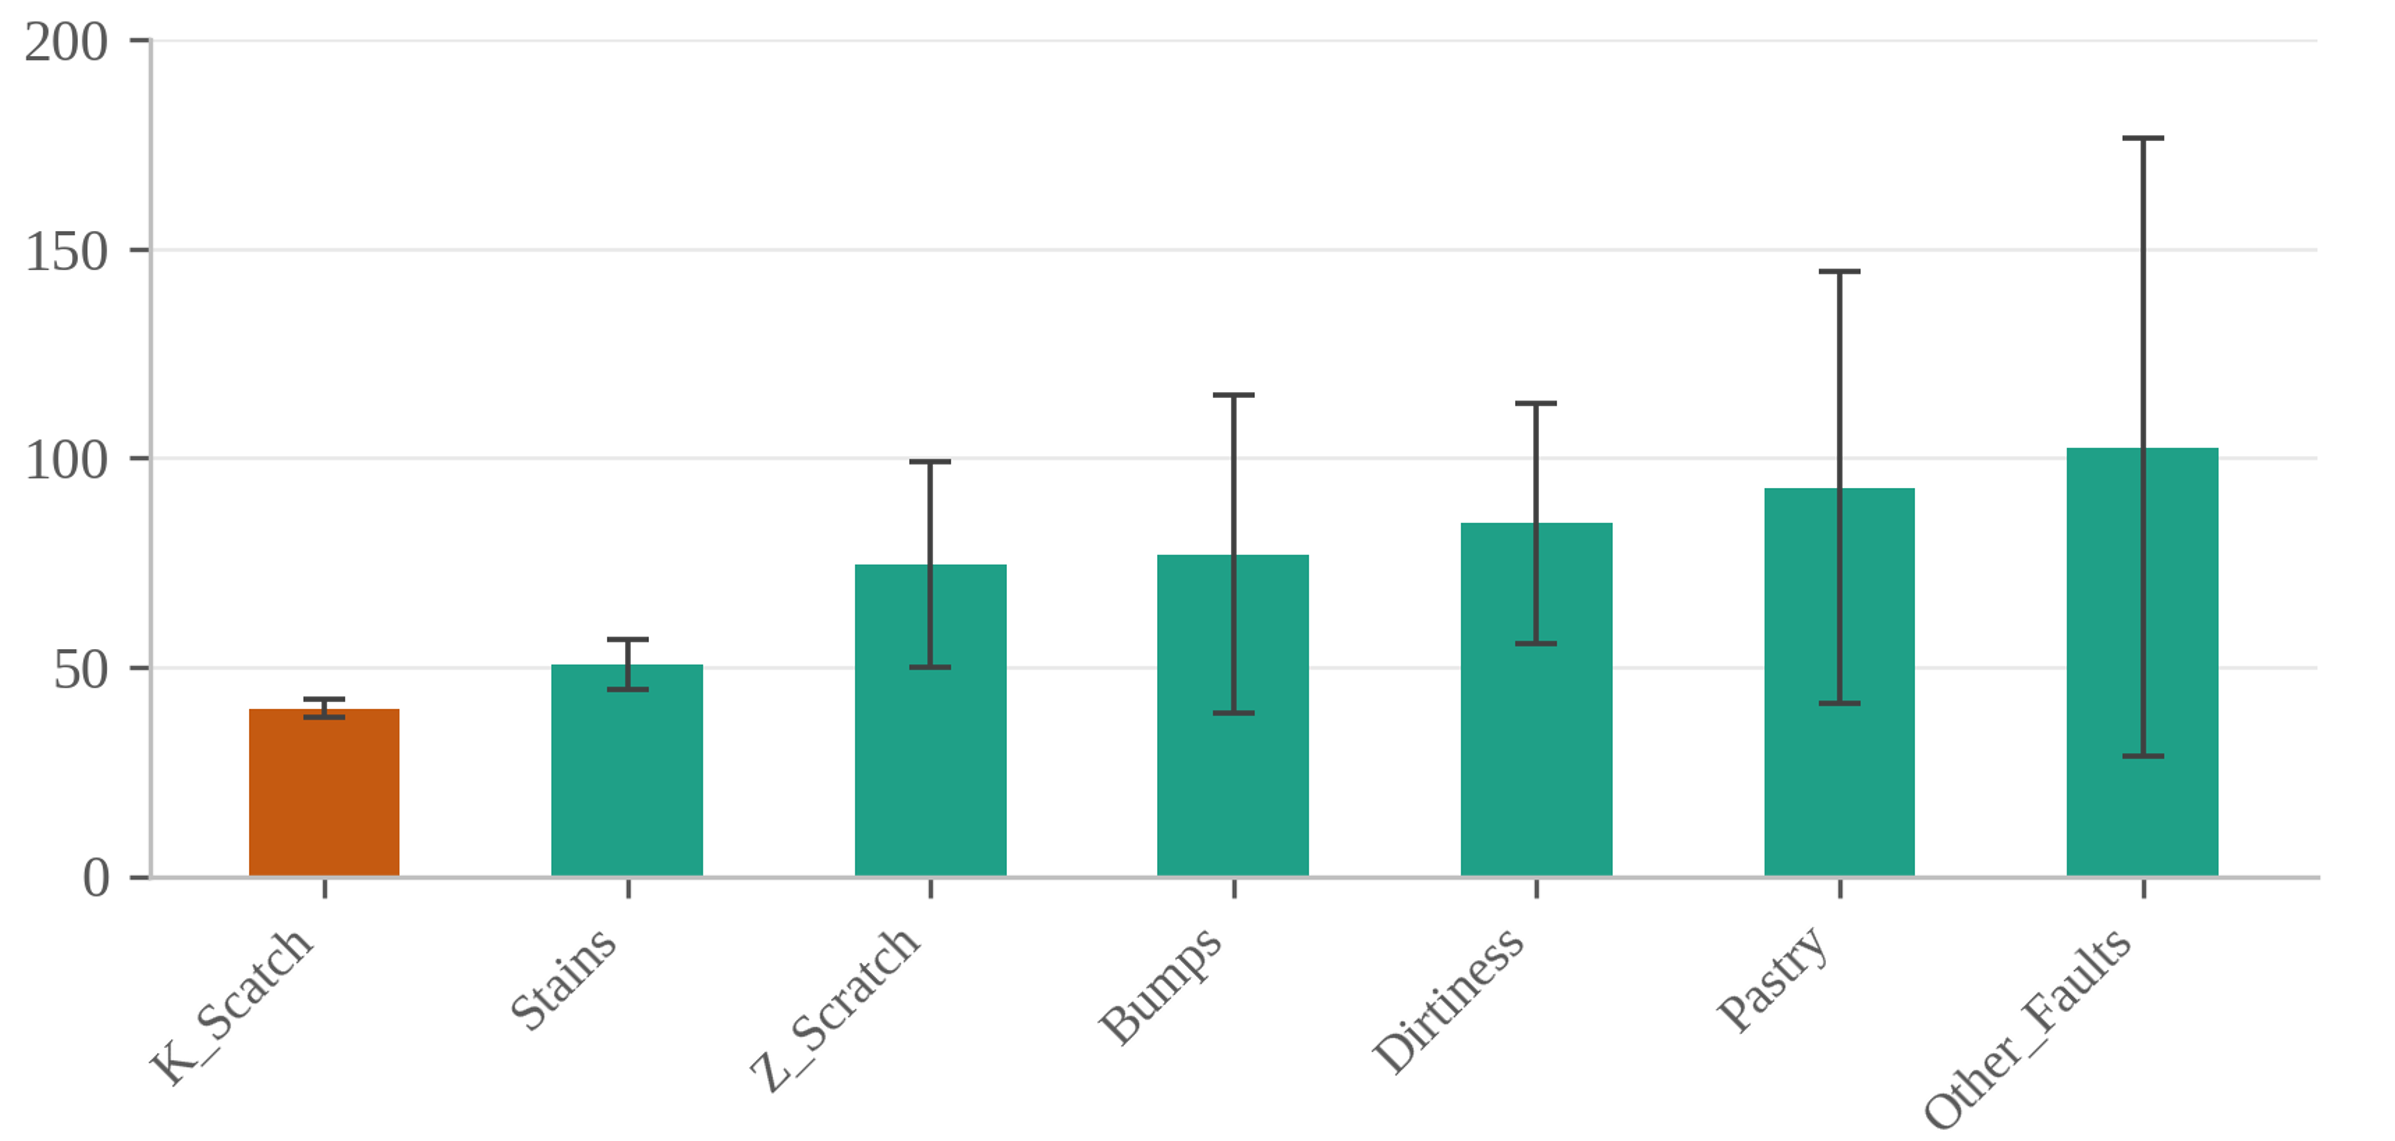
\includegraphics[width=1.0\linewidth]{Figures/fig07_column1.png}
            %\begin{figurecaptionmodern}
            \capfig{Độ dày trung bình theo loại lỗi.}
            %\end{figurecaptionmodern}
        \end{figure}
    \end{minipage}
    &
    \justifying \noindent Hình 9 mô tả độ dày trung bình theo loại lỗi. Thanh dọc là độ lệch chuẩn mẫu của từng nhãn chứ không phải khoảng tin cậy. Chiều cao cột không chênh nhau nhiều, nhưng độ phân tán thì rất khác nhau. Other\_Faults phân tán nhất với SD mẫu 73,85, còn K\_Scatch gần như không dao động với SD mẫu 2,20.
\end{tabular}
\end{table}



\noindent
\textbf{Bước 5. Dựng Pivot Table độ dày theo loại lỗi $\times$ dòng thép}

\noindent
Câu hỏi đặt ra cho lớp phân tích cuối là trên mỗi dòng thép, từng loại lỗi xuất hiện ở mức độ dày nào?
\begin{enumerate}
  \item Chọn toàn bộ vùng dữ liệu.
  \item Chọn Insert → PivotTable → chọn vị trí đặt Pivot Table.
  \item Kéo thả sao cho vùng Rows nhận Fault\_Type\_Clean, vùng Columns nhận SteelType, vùng Values nhận Steel\_Plate\_Thickness.
  \item Tại PivotTable Fields, nhấn vào trường giá trị vừa kéo → Value Field Settings → Average.
\end{enumerate}

% Hinh nay da duoc dung lai tu workbook 1.941 ban ghi (nguon: figures_src/build_tables.py). Khong can chup lai tu Excel.

\begin{table}[H]
\centering
\begin{tabular}{@{}m{0.65\linewidth} m{0.32\linewidth}@{}}
    \begin{minipage}{\linewidth}
        \vspace{-3em}
        \begin{figure}[H]
            \centering
            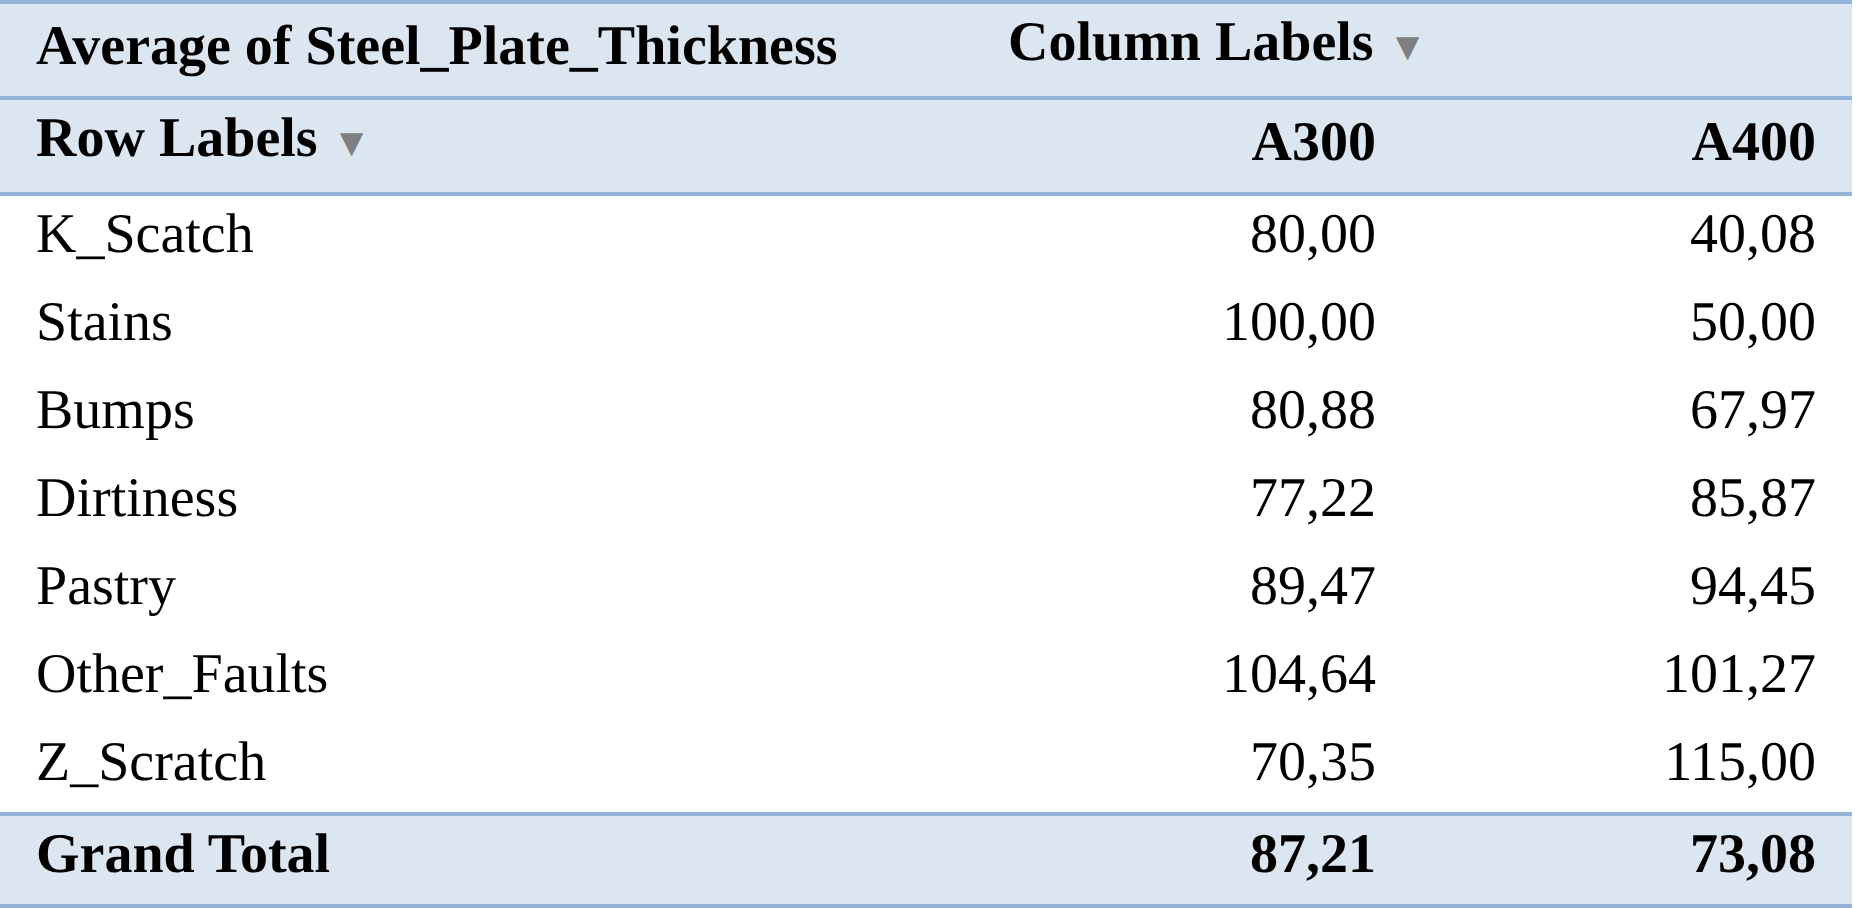
\includegraphics[width=1.0\linewidth]{Figures/fig08_bang_do_day_theo_loai_thep.png}
            %\begin{figurecaptionmodern}
            \capfig{Độ dày trung bình theo loại lỗi và dòng thép.}
            %\end{figurecaptionmodern}
        \end{figure}
    \end{minipage}
    &
    \justifying \noindent Hình 10 trình bày độ dày trung bình theo loại lỗi và dòng thép, tính trên 1.941 bản ghi. Cùng một loại lỗi nhưng mức độ dày đặc trưng trên hai dòng thép có thể khác nhau xa, với điều kiện đọc kèm số lượng vết ở mỗi ô (xem lưu ý tại Bước 7).
\end{tabular}
\end{table}



\noindent
\textbf{Bước 6. Vẽ biểu đồ cột}

\begin{enumerate}
  \item Chọn Pivot Table → PivotTable Analyze → PivotChart.
  \item Chọn biểu đồ cột (Clustered Column) → OK.
  \item Điều chỉnh và đặt tiêu đề cho biểu đồ.
\end{enumerate}

% Hinh nay da duoc dung lai tu workbook 1.941 ban ghi (nguon: figures_src/build_charts.py).

\begin{table}[H]
\centering
\begin{tabular}{@{}m{0.65\linewidth} m{0.32\linewidth}@{}}
    \begin{minipage}{\linewidth}
        \vspace{-6em}
        \begin{figure}[H]
            \centering
            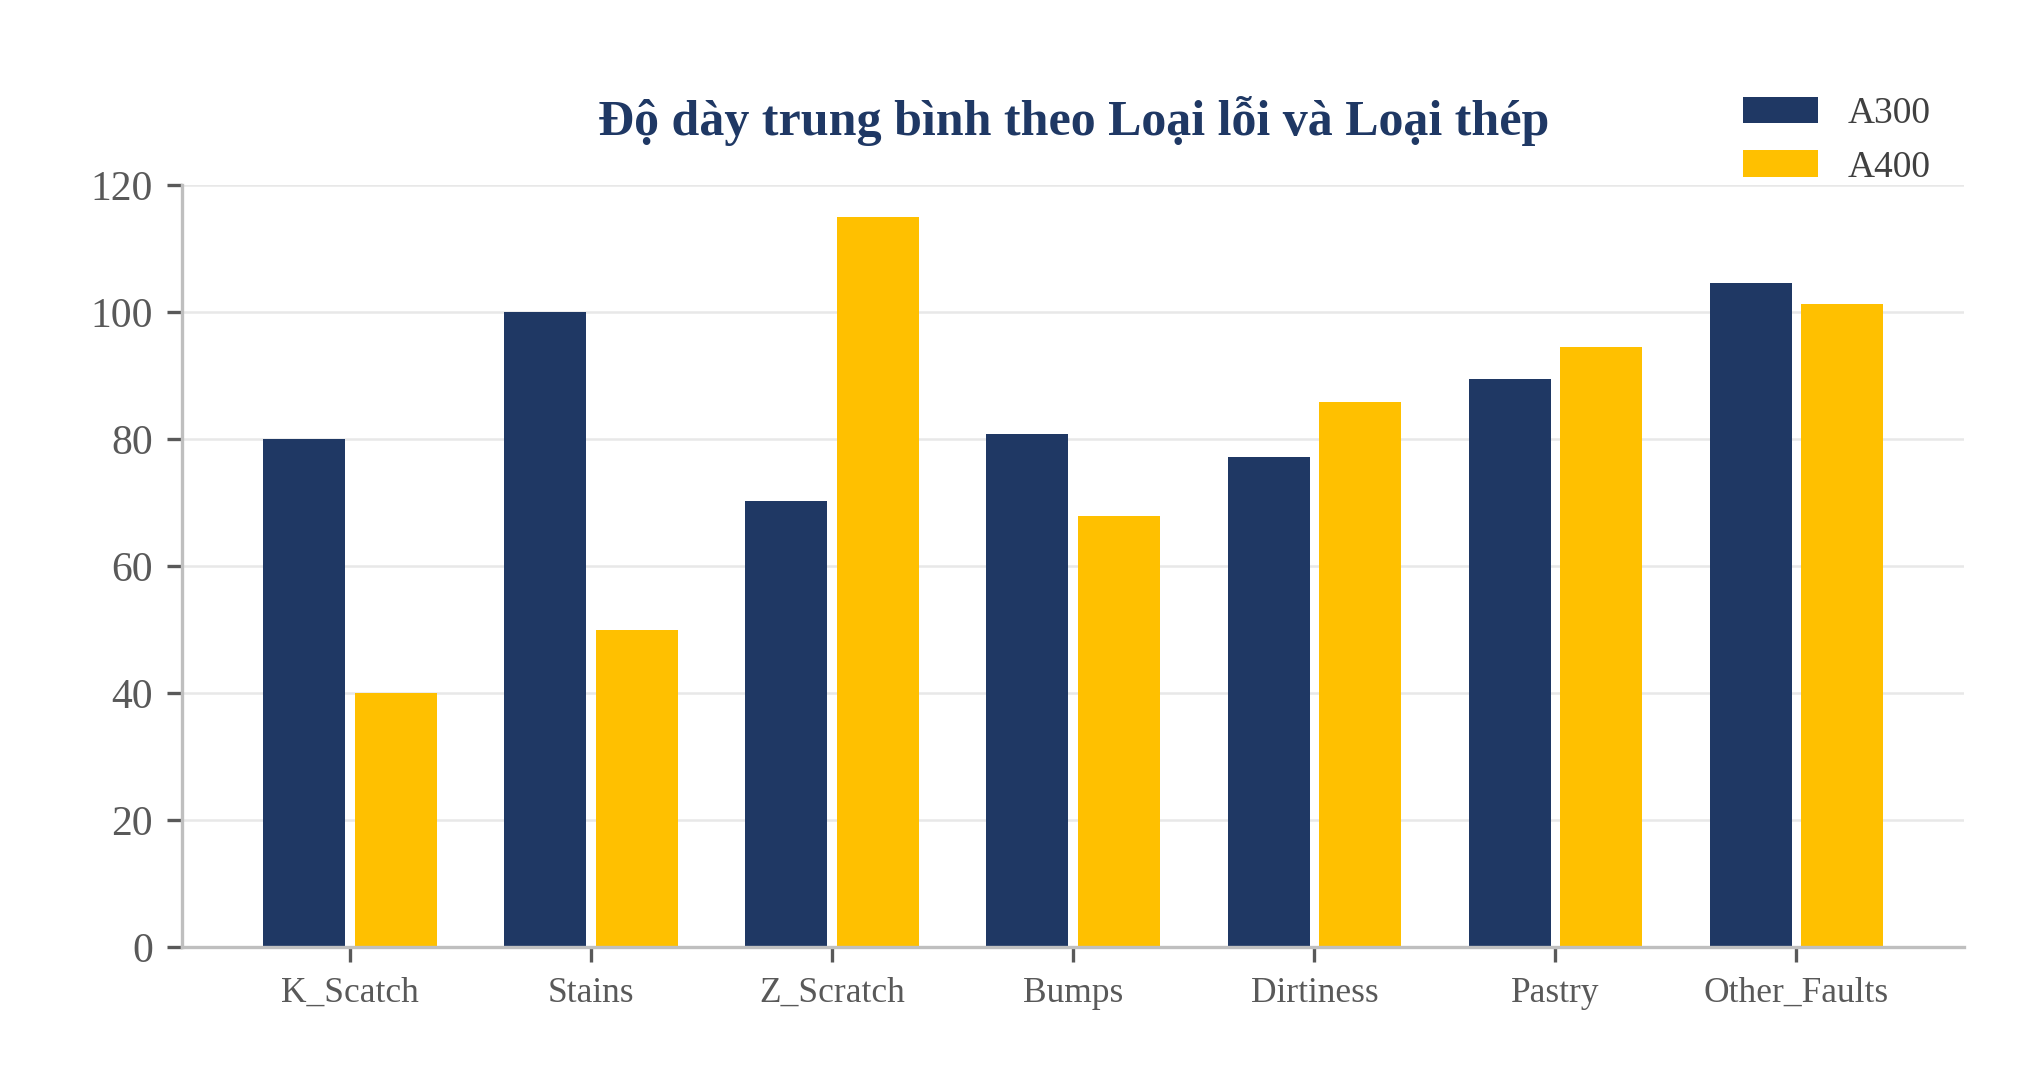
\includegraphics[width=1.0\linewidth]{Figures/fig09_column.png}
            %\begin{figurecaptionmodern}
            \capfig{Độ dày trung bình theo loại lỗi và dòng thép.}
            %\end{figurecaptionmodern}
        \end{figure}
    \end{minipage}
    &
    \justifying \noindent Hình 11 trình bày biểu đồ độ dày trung bình theo loại lỗi và dòng thép, trên 1.941 bản ghi. Chênh lệch giữa hai cột trong cùng một loại lỗi là điểm cần soi tiếp, nhưng chỉ đọc được ở những loại lỗi có đủ số vết trên cả hai dòng thép. K\_Scatch và Stains mỗi loại chỉ có đúng 1 vết ở phía A300, nên cột A300 của hai nhãn đó không mang thông tin thống kê.
\end{tabular}
\end{table}


\noindent
\textbf{Bước 7. Đọc nhận định để trả lời Q4}

\begin{itemize}
  \item \textbf{Phân bố tổng thể lệch hẳn về tấm mỏng.} Các tấm thép có vết lỗi mang độ dày trung bình 78,74, trung vị 70 và độ lệch chuẩn mẫu 55,09. Đây là phân phối lệch phải mạnh, với những tấm rất dày (tới 300) kéo trung bình lên cao hơn trung vị.
  \item \textbf{Khoảng ba phần tư số vết lỗi nằm ở dải độ dày từ 40 đến 80} (1.481 trên 1.941 bản ghi, tương đương 76,30\%), trong đó mức 40 vừa là giá trị nhỏ nhất vừa là mức xuất hiện nhiều nhất. Cần đọc kèm giới hạn về mẫu số đã nêu ở đầu mục. Bảng chỉ chứa vết lỗi, không chứa sản lượng, nên con số này mô tả \emph{tập vết lỗi} chứ chưa nói được nhóm sản phẩm nào dễ lỗi hơn. Muốn kết luận điều đó cần thêm sản lượng theo từng mức độ dày.
  \item \textbf{K\_Scatch dồn gần như toàn bộ vào mức độ dày 40.} Độ lệch chuẩn mẫu của nhóm chỉ là 2,20, thấp nhất trong bảy loại lỗi và nhỏ hơn mức chung 55,09 khoảng 25 lần. Ghép với kết quả Mục VII.1 (99,74\% số vết trên thép A400), K\_Scatch có một mô tả rất hẹp, gần như chỉ xuất hiện trên một dòng thép và ở một mức độ dày. Một khuôn chặt như vậy khó đến từ biến động ngẫu nhiên, nên đây là chỗ đáng mang ra hiện trường kiểm chứng trước tiên. Bản thân dữ liệu chưa cho biết điều gì tạo ra khuôn đó, vì bảng không chứa biến vận hành nào.
  \item \textbf{Other\_Faults có trung bình lẫn độ phân tán lớn nhất}, đúng như dự đoán về một nhóm gộp không đồng nhất. Con số trung bình của nó là trung bình của nhiều hiện tượng khác nhau nên không đại diện cho hiện tượng nào. Thêm một lần nữa, kết luận cần tách nhỏ nhóm này được củng cố.
  \item \textbf{Chênh lệch độ dày giữa hai dòng thép cần đọc thận trọng.} Trên bảng Pivot chéo, K\_Scatch và Stains hiện chênh lệch rất lớn giữa A300 và A400, nhưng phía A300 của hai loại lỗi này chỉ có đúng 1 vết, nên con số trung bình phía đó không có ý nghĩa thống kê. Kết luận đúng là các loại lỗi này gần như chỉ tồn tại trên một dòng thép, và trên chính dòng đó chúng có mức độ dày đặc trưng riêng. Với Z\_Scratch (172 vết A300, 18 vết A400), chênh lệch giữa hai dòng là có thật, nhưng phía A400 chỉ có 18 bản ghi nên con số 115 cũng cần đọc thận trọng. Điều rút ra được ở mức chắc chắn nhất là phân bố lỗi của hai dòng thép khác nhau đủ rõ để không nên gộp chung khi theo dõi. Việc hai dòng có cần hai quy trình kiểm tra khác nhau hay không thì phải kiểm chứng bằng dữ liệu sản lượng và biến vận hành, chưa trả lời được từ bảng này.
\end{itemize}

\section{Dashboard}

Các phân tích ở Mục VII trả lời câu hỏi tại một thời điểm. Dashboard là công cụ để việc theo dõi đó diễn ra \emph{thường xuyên} mà không cần lặp lại phân tích. Toàn bộ bảng số liệu và biểu đồ rời rạc được gom về một màn hình thống nhất, nhờ đó người quản lý nhìn một lần là nắm được tình hình chất lượng, cơ cấu các loại lỗi và khác biệt giữa hai dòng thép. Thành phần tương tác trung tâm là \emph{Slicer}, bộ nút lọc trực quan của Excel gắn với Pivot Table. Khi bấm chọn một dòng thép hoặc một giá trị ngày, mọi biểu đồ nối với Slicer đó lập tức cập nhật theo. Cần nhớ cột ngày là biến mô phỏng, nên bộ lọc này minh họa thao tác chứ không dùng để theo dõi chất lượng theo thời gian.

\subsection{Thiết kế bố cục Dashboard}

\textbf{Bước 1. Tạo sheet Dashboard}

\begin{enumerate}
  \item Tạo sheet mới, đổi tên thành Dashboard.
  \item Ẩn lưới ô cho nền sạch bằng tab View → bỏ tick Gridlines.
\end{enumerate}

\noindent
\textbf{Bước 2. Quy hoạch vùng}

\noindent
Màn hình được chia thành các vùng chức năng, đọc từ trên xuống theo đúng thứ tự người xem cần, bắt đầu bằng tiêu đề, tiếp đến các con số tổng quan, sau đó là bộ lọc và biểu đồ, và cuối cùng là phần diễn giải.

\begin{itemize}
  \item Header, tức tiêu đề dashboard, đặt ở vùng A1:W2.
  \item 4 thẻ KPI (tổng số bản ghi, số loại lỗi, số giá trị ngày mô phỏng, tỷ lệ vượt ngưỡng IQR của \texttt{Pixels\_Areas}) đặt ở vùng A3:W5.
  \item Slicer (lọc theo dòng thép và theo giá trị ngày mô phỏng) đặt ở vùng A6:B27.
  \item Biểu đồ 1 đặt ở vùng C6:M16.
  \item Biểu đồ 2 đặt ở vùng N6:W16.
  \item Biểu đồ 3 đặt ở vùng C18:K27.
  \item Textbox Nhận định, tóm tắt các phát hiện chính, đặt ở vùng M18:W27.
\end{itemize}

\subsection{Dashboard hoàn chỉnh}

% Anh dashboard giu nguyen thiet ke goc; chi cap nhat o KPI 'Ty le outlier dien tich' tu 24,0% thanh 20,35% (395/1.941).
\begin{figure}[H]
    \centering
    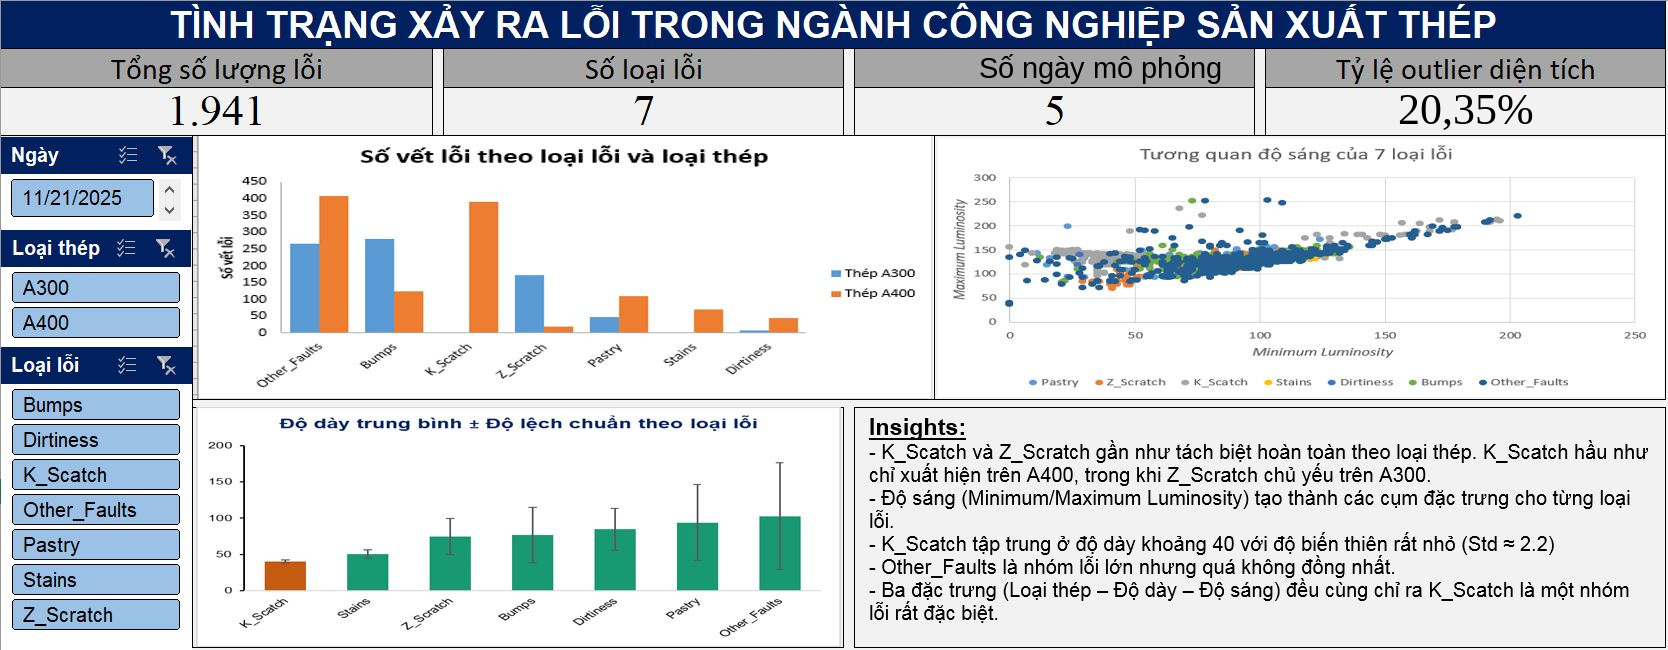
\includegraphics[width=1.0\linewidth]{Figures/fig10_dashboard.jpg}
    \begin{figurecaptionmodern}
    \capfig{Dashboard hoàn chỉnh, dựng trên đúng 1.941 dòng dữ liệu đã làm sạch. Toàn bộ kết quả phân tích gói trong một màn hình, gồm thẻ KPI tổng quan, biểu đồ cơ cấu lỗi và bộ lọc Slicer theo dòng thép và theo giá trị ngày mô phỏng. Thẻ KPI thứ tư là tỷ lệ bản ghi vượt ngưỡng IQR của \texttt{Pixels\_Areas}, bằng 20,35\%.}
    \end{figurecaptionmodern}
\end{figure}

\clearpage
\section{Nhận định}

Mục này gom các phát hiện của toàn bộ quá trình phân tích. Cách xếp hạng ở đây là theo \textbf{mức độ chắc chắn của bằng chứng}, không theo mức độ nghiêm trọng. Lý do nằm ở giới hạn đã nêu tại Mục I.4. Bảng dữ liệu không chứa chi phí thiệt hại, không chứa mức hạ cấp sản phẩm và không chứa sản lượng, nên không có căn cứ nào để nói lỗi nào gây tổn thất lớn hơn lỗi nào.

\noindent
Ba nhóm dưới đây khác nhau ở một điểm cụ thể. Nhóm A kiểm chứng lại được ngay bằng chính bảng dữ liệu. Nhóm B đọc được từ dữ liệu nhưng cần thêm bằng chứng bên ngoài mới kết luận được. Nhóm C là những gì bộ dữ liệu này không cho phép nói.\medskip

\noindent
\textbf{A. Phát hiện mô tả, kiểm chứng lại được bằng chính bảng dữ liệu}

\begin{itemize}
    \item \textbf{Ba nhãn lớn nhất chiếm 75,53\% toàn bộ bản ghi} (Mục VII.1). Other\_Faults 673, Bumps 402 và K\_Scatch 391, cộng lại 1.466 trên 1.941. Nhãn nhỏ nhất là Dirtiness với 55 bản ghi, bằng 2,83\%. Mức mất cân bằng này quyết định cách đánh giá mọi mô hình phân loại về sau, vì một mô hình luôn đoán nhãn lớn nhất đã đạt 34,67\%.

    \item \textbf{Ba nhãn gắn gần như tuyệt đối với một dòng thép} (Mục VII.1). K\_Scatch có 390 trên 391 bản ghi nằm trên A400 (99,74\%), Stains có 71 trên 72 trên A400 (98,61\%), Z\_Scratch có 172 trên 190 trên A300 (90,53\%). Cả ba đều vượt ngưỡng phán quyết 90\% đặt trước ở Mục V.

    \item \textbf{K\_Scatch có độ phân tán độ dày nhỏ nhất trong bảy nhãn} (Mục VII.3). Trung bình 40,18 với độ lệch chuẩn mẫu 2,20, so với độ lệch chuẩn chung của cả bảng là 55,09. Ghép với gạch đầu dòng trên, K\_Scatch dồn gần như toàn bộ vào một dòng thép và một mức độ dày.

    \item \textbf{Other\_Faults là nhãn gộp, và là nhãn phân tán nhất ở mọi chiều} (Mục VII.1 đến VII.3). Nhãn này chiếm 673 bản ghi (34,67\%), có độ dày trung bình cao nhất (102,60) và độ lệch chuẩn mẫu lớn nhất (73,85). Mọi thống kê tính trên nhãn này là trung bình của nhiều hiện tượng khác nhau cộng lại, nên không đại diện cho hiện tượng nào.

    \item \textbf{Độ sáng tách được đúng một nhãn} (Mục VII.2). K\_Scatch có trung vị \texttt{Minimum\_of\_Luminosity} bằng 41, trong khi các nhãn còn lại nằm trong khoảng 80 đến 97. Sáu nhãn kia chồng lấn nhau trên cả hai trục độ sáng.

    \item \textbf{Bảng đã làm sạch trùng khớp với bản gốc trên từng ô} (Mục VI). Đây là phát hiện có bằng chứng mạnh nhất của báo cáo, vì nó dựa trên một nguồn hoàn toàn độc lập với mọi thứ bài tự dựng ra. Đối chiếu 27 biến trên cả 1.941 bản ghi, tức 52.407 ô, cho \textbf{0 ô lệch}, và nhãn \texttt{Faults} cũng khớp trên mọi bản ghi. Kết quả này xác nhận cả năm bước can thiệp ở Mục VI, gồm 67 ô từng bị trống và 16 giá trị phái sinh đã sửa, đều khôi phục đúng giá trị thật. Câu hỏi Q0 vì vậy được trả lời ở mức chắc chắn cao nhất mà một bài phân tích có thể đạt được, và mọi con số ở nhóm A dưới đây đứng trên nền đó.
\end{itemize}

\noindent
\textbf{B. Nhận định khám phá, cần thêm bằng chứng bên ngoài}

\begin{itemize}
    \item \textbf{Một quy tắc hai ngưỡng nhận được phần lớn K\_Scatch} (Mục VII.2). Quy tắc Min $<$ 50 và Max $>$ 120 đạt precision 86,77\% và recall 72,12\%. Hai con số này đo trên chính tập đã dùng để chọn ngưỡng nên chắc chắn lạc quan, và chỉ có nghĩa sau khi đo lại trên một tập kiểm tra độc lập.

    \item \textbf{Có dấu hiệu một nhóm con thuần nhất nằm trong Other\_Faults} (Mục VII.2). Ở 140 bản ghi có Min $>$ 120, hiệu Max $-$ Min có trung vị 19 và khoảng tứ phân vị 17 đến 23, và Other\_Faults chiếm 74 trong số đó. Đây là một hướng tách nhãn đáng thử, chưa phải một kết luận.

    \item \textbf{Cùng một nhãn có mức độ dày khác nhau trên hai dòng thép} (Mục VII.3). Rõ nhất là Z\_Scratch, trung bình 70,35 trên A300 so với 115,00 trên A400. Cần thận trọng vì phía A400 chỉ có 18 bản ghi. Với K\_Scatch và Stains thì phía A300 chỉ có đúng 1 bản ghi, nên chênh lệch hiển thị trên bảng Pivot không mang thông tin thống kê.
\end{itemize}

\noindent
\textbf{C. Những gì bộ dữ liệu này không cho phép kết luận}

\begin{itemize}
    \item \textbf{Không kết luận được về nguyên nhân.} Các khuôn ở nhóm A đều là liên hệ trong mẫu. Bảng không chứa biến vận hành, mã thiết bị hoặc mã ca sản xuất, nên không có đường nào đi từ những khuôn đó tới một nguyên nhân cụ thể.
    \item \textbf{Không xếp hạng được mức độ nghiêm trọng.} Thiếu chi phí thiệt hại và mức hạ cấp sản phẩm.
    \item \textbf{Không tính được tỷ lệ lỗi.} Thiếu sản lượng làm mẫu số, nên mọi tỷ lệ trong báo cáo đều là tỷ trọng trong nội bộ tập vết lỗi.
    \item \textbf{Không nói được gì về thời gian.} Cột \texttt{Production\_Date} là biến mô phỏng.
    \item \textbf{Không phát biểu được về cơ chế vật lý của từng nhãn}, vì nguồn không công bố định nghĩa nhãn và không công bố đơn vị đo.
\end{itemize}

\begin{guidelinebox}{Một phát hiện của bài này tự vạch giới hạn của chính nó}
Phát hiện chắc nhất của báo cáo là K\_Scatch dồn vào một dòng thép và một mức độ dày. Chính độ chặt đó lại là thứ khiến nó \emph{không} kiểm chứng được từ bên trong bộ dữ liệu. Vì gần như toàn bộ K\_Scatch nằm ở cùng một điểm trên cả hai chiều, không còn biến thiên nào để tách xem dòng thép hay độ dày mới là yếu tố đi kèm, hay cả hai chỉ cùng phản ánh một đợt sản xuất nào đó. Trả lời câu này bắt buộc phải có dữ liệu vận hành, và đó là nội dung Giai đoạn 2 ở mục sau.
\end{guidelinebox}


\clearpage
\section{Khuyến nghị}

Mục IX kết thúc bằng một danh sách các khuôn đo được và một danh sách những gì bộ dữ liệu không cho phép nói. Phần khuyến nghị chuyển hai danh sách đó thành việc phải làm.

\noindent
Điểm cần thống nhất trước là bản chất của các khuyến nghị này. Vì mọi phát hiện ở Mục IX đều là liên hệ trong mẫu, không có phát hiện nào đủ để đề xuất một can thiệp vật lý lên dây chuyền. Ba giai đoạn dưới đây vì vậy là một \textbf{kế hoạch kiểm chứng}, đi từ việc chốt lại nền dữ liệu, sang việc thu thập đúng những biến còn thiếu, rồi mới tới việc thử nghiệm dự báo. Mỗi giai đoạn có một điều kiện hoàn tất kiểm được, và giai đoạn sau chỉ bắt đầu khi giai đoạn trước đạt.\medskip

\noindent
\textbf{1) Giai đoạn 1 (0 đến 30 ngày) chốt lại nền dữ liệu và bản báo cáo.}

\noindent
Mục tiêu của giai đoạn này là đưa mọi con số về trạng thái truy được nguồn, việc không cần thêm dữ liệu bên ngoài nào.

\begin{itemize}
  \item Phép đối chiếu toàn bảng với bản gốc đã chạy và cho 0 ô lệch (Mục VI). Việc còn lại là lưu kết quả đó thành một hồ sơ chạy được lại, gồm bản \texttt{Faults.NNA} kèm mã băm, mã ghép bảng, và bảng kết quả theo từng biến. Điều kiện hoàn tất là người khác chạy lại hồ sơ này cũng ra 0 ô lệch.
  \item Lập nhật ký thay đổi cho toàn bộ 67 ô từng bị trống và 16 giá trị phái sinh đã sửa, ghi rõ giá trị cũ, giá trị mới và căn cứ. Điều kiện hoàn tất là mỗi dòng nhật ký chỉ về được một căn cứ cụ thể.
  \item Đưa Dashboard ở Mục VIII vào dùng như một công cụ theo dõi phân bố, với điều kiện các thẻ KPI chỉ hiển thị số đếm và tỷ trọng, không hiển thị chỉ tiêu chất lượng nào cần mẫu số sản lượng.
\end{itemize}

\noindent
\textbf{2) Giai đoạn 2 (1 đến 3 tháng) thu thập biến còn thiếu và xác nhận tại hiện trường.}

\noindent
Mục tiêu là bổ sung đúng những biến mà Mục IX.C đã chỉ ra là thiếu, để các khuôn ở Mục IX.A có thể được kiểm chứng thay vì chỉ được mô tả.

\begin{itemize}
  \item Thu thập sản lượng theo dòng thép và theo từng mức độ dày. Đây là mẫu số còn thiếu, và là điều kiện để lần đầu tiên tính được tỷ lệ lỗi thay vì tỷ trọng.
  \item Thu thập biến vận hành và mã định danh, gồm mã tấm, mã cuộn, mã thiết bị, mã ca, nhiệt độ cán, tốc độ dây chuyền, tuổi con lăn. Không có nhóm biến này thì mọi câu hỏi về nguyên nhân đều nằm ngoài tầm với.
  \item Mang khuôn K\_Scatch ra hiện trường kiểm chứng. Câu hỏi cụ thể đặt cho bộ phận sản xuất là dòng A400 ở mức độ dày 40 có gì khác các nhóm sản phẩm còn lại về thiết bị, thiết lập hoặc lịch bảo trì. Điều kiện hoàn tất là một câu trả lời có hoặc không kèm bằng chứng, không phải một giả thuyết mới.
  \item Cùng bộ phận QC chốt định nghĩa cho bảy nhãn và tách nhỏ Other\_Faults. Hướng tách đáng thử trước là nhóm con có Min $>$ 120 đã mô tả ở Mục IX.B.
  \item Ghi nhận đơn vị đo thật của các biến, bắt đầu từ \texttt{Steel\_Plate\_Thickness}. Chừng nào chưa có, báo cáo tiếp tục viết các con số này không kèm đơn vị.
\end{itemize}

\noindent
\textbf{3) Giai đoạn 3 (3 đến 6 tháng) thử nghiệm dự báo có tập kiểm tra độc lập.}

\noindent
Giai đoạn này chỉ bắt đầu khi Giai đoạn 2 đã có dữ liệu, vì thử nghiệm dự báo trên bộ dữ liệu hiện tại sẽ cho những con số không kiểm chứng được.

\begin{itemize}
  \item Chia dữ liệu thành tập huấn luyện và tập kiểm tra độc lập trước khi chọn bất kỳ ngưỡng nào. Đo lại quy tắc K\_Scatch ở Mục VII.2 trên tập kiểm tra. Điều kiện hoàn tất là một cặp precision và recall đo trên dữ liệu chưa từng tham gia chọn ngưỡng.
  \item Nếu quy tắc một dòng vẫn đạt trên tập độc lập, xây mô hình phân loại đầy đủ, xử lý mất cân bằng lớp và đánh giá bằng F1 theo từng lớp hoặc trung bình macro thay vì accuracy, theo đúng lập luận ở Mục VII.1.
  \item Chạy thử song song với quy trình QC hiện tại trên một phạm vi hẹp, so kết quả của mô hình với kết luận của người kiểm tra, và chỉ mở rộng khi có đủ số ca đối chiếu.
\end{itemize}

\begin{guidelinebox}{Điều kiện để một khuyến nghị vượt lên thành hành động vật lý}
Không khuyến nghị nào ở trên đề xuất chỉnh thiết bị, hiệu chuẩn camera hoặc đổi quy trình kiểm tra. Đó là chủ ý, vì bộ dữ liệu hiện tại không chứa biến nào cho phép nối một khuôn thống kê với một nguyên nhân vật lý.

Một khuyến nghị chỉ được nâng lên thành hành động vật lý khi có đủ ba thứ, gồm một biến vận hành đo được cùng thay đổi với khuôn đã quan sát, một lần xác nhận tại hiện trường, và một phép đo trước sau trên chính chỉ tiêu mà can thiệp nhắm tới. Thiếu bất kỳ thứ nào trong ba, việc đúng phải làm vẫn là thu thập thêm dữ liệu.
\end{guidelinebox}

% =====================================================================
% =====================================================================
\clearpage
\section*{Tài liệu tham khảo}
\addcontentsline{toc}{section}{Tài liệu tham khảo}

\noindent \textbf{Dữ liệu và tài liệu kèm theo}

\noindent Toàn bộ số liệu trong báo cáo tái lập được từ các file dưới đây. File Excel lời giải giữ nguyên các cột kiểm tra và các Pivot Table trung gian, nên người đọc có thể mở từng sheet để chạy lại mọi bước theo đúng trình tự của Mục VI đến VIII.

\begin{center}
\url{https://drive.google.com/drive/folders/1IpAVZb8KNwpU70SmD1EIYvCwqX6MM4N4}
\end{center}

\noindent Thư mục gồm ba tài liệu.

\begin{itemize}
  \item \textbf{Bộ dữ liệu thực hành, bản thô.} \texttt{data\_chua\_sach\_ko\_sua.xlsx}, 1.961 dòng $\times$ 29 cột, sheet \texttt{Faults}. Đây là bản đã được bổ sung cột ngày mô phỏng và cố ý đưa vào một số lỗi dữ liệu phục vụ mục đích thực hành, tức là điểm xuất phát của Mục VI.
  \item \textbf{File Excel lời giải và Dashboard.} \texttt{PivotTableDashboard\_1941.xlsx}, gồm sheet dữ liệu đã làm sạch 1.941 dòng kèm các cột bổ trợ và cột kiểm tra (từ AD đến AT), các sheet Pivot Table và biểu đồ của Mục VII, và sheet Dashboard của Mục VIII. Mọi bảng và hình trong báo cáo đều truy được về file này.
  \item \textbf{Bản PDF của chính báo cáo này}, để đối chiếu khi người đọc chạy lại từng bước.
\end{itemize}

\noindent Bộ dữ liệu gốc \emph{Steel Plates Faults}~\cite{steelplates2010} gồm 1.941 bản ghi và 27 đặc trưng, tải trực tiếp được từ UCI Machine Learning Repository theo địa chỉ dưới đây.

\begin{center}
\url{https://archive.ics.uci.edu/dataset/198/steel+plates+faults}\\[2pt]
DOI \url{https://doi.org/10.24432/C5J88N}
\end{center}

\noindent Bản dùng để đối chiếu ở Mục VI là file \texttt{Faults.NNA} trong gói tải về từ liên kết trên, dung lượng 299.482 byte, mã băm SHA-256 bắt đầu bằng \texttt{08994f5b}. Ghi lại mã băm để người đọc chắc chắn đang đối chiếu với đúng phiên bản mà báo cáo đã dùng. Mọi con số trong báo cáo tái lập được với điều kiện người đọc dùng đúng bản 1.941 bản ghi đã loại trùng nêu trên cùng các công thức đã ghi trong Mục VI và Mục VII.

\vspace{0.4em}
\noindent \textbf{Lịch sử dữ liệu}

\noindent Các bản phân tích ban đầu của báo cáo đều sử dụng 1.941 bản ghi. Một dòng trùng phát sinh trong vùng nguồn dùng để hoàn thiện Dashboard đã được loại bỏ trước khi tái xuất các bảng và biểu đồ của bản này. Toàn bộ chín hình từ Hình 3 đến Hình 11 được dựng lại từ đúng nguồn 1.941 bản ghi, không lấy từ ảnh chụp cũ, và mã dựng hình kèm theo trong thư mục nguồn. Ảnh Dashboard ở Hình 12 giữ nguyên thiết kế gốc, chỉ cập nhật hai chỗ chữ là tỷ lệ vượt ngưỡng IQR và nhãn của thẻ KPI về cột ngày.

\vspace{0.4em}
\noindent \textbf{Tài liệu trích dẫn}

\printbibliography[heading=none]

\end{document}